\documentclass[a4paper]{book}
\usepackage{makeidx}
\usepackage{natbib}
\usepackage{graphicx}
\usepackage{multicol}
\usepackage{float}
\usepackage{listings}
\usepackage{color}
\usepackage{ifthen}
\usepackage[table]{xcolor}
\usepackage{textcomp}
\usepackage{alltt}
\usepackage{ifpdf}
\ifpdf
\usepackage[pdftex,
            pagebackref=true,
            colorlinks=true,
            linkcolor=blue,
            unicode
           ]{hyperref}
\else
\usepackage[ps2pdf,
            pagebackref=true,
            colorlinks=true,
            linkcolor=blue,
            unicode
           ]{hyperref}
\usepackage{pspicture}
\fi
\usepackage[utf8]{inputenc}
\usepackage[french]{babel}

\usepackage{mathptmx}
\usepackage[scaled=.90]{helvet}
\usepackage{courier}
\usepackage{sectsty}
\usepackage[titles]{tocloft}
\usepackage{doxygen}
\lstset{language=C++,inputencoding=utf8,basicstyle=\footnotesize,breaklines=true,breakatwhitespace=true,tabsize=8,numbers=left }
\makeindex
\setcounter{tocdepth}{3}
\renewcommand{\footrulewidth}{0.4pt}
\renewcommand{\familydefault}{\sfdefault}
\hfuzz=15pt
\setlength{\emergencystretch}{15pt}
\hbadness=750
\tolerance=750
\begin{document}
\hypersetup{pageanchor=false,citecolor=blue}
\begin{titlepage}
\vspace*{7cm}
\begin{center}
{\Large \-Cluedo \\[1ex]\large 1.\-0 }\\
\vspace*{1cm}
{\large \-Généré par Doxygen 1.7.6.1}\\
\vspace*{0.5cm}
{\small Mercredi Novembre 27 2013 11:16:50}\\
\end{center}
\end{titlepage}
\clearemptydoublepage
\pagenumbering{roman}
\tableofcontents
\clearemptydoublepage
\pagenumbering{arabic}
\hypersetup{pageanchor=true,citecolor=blue}
\chapter{\-Index des classes}
\section{\-Hiérarchie des classes}
\-Cette liste d'héritage est classée approximativement par ordre alphabétique \-:\begin{DoxyCompactList}
\item \contentsline{section}{\-Bouton}{\pageref{classBouton}}{}
\item \contentsline{section}{\-Carte}{\pageref{classCarte}}{}
\begin{DoxyCompactList}
\item \contentsline{section}{\-Carte\-Arme}{\pageref{classCarteArme}}{}
\item \contentsline{section}{\-Carte\-Personnage}{\pageref{classCartePersonnage}}{}
\item \contentsline{section}{\-Carte\-Piece}{\pageref{classCartePiece}}{}
\end{DoxyCompactList}
\item \contentsline{section}{\-Case}{\pageref{classCase}}{}
\begin{DoxyCompactList}
\item \contentsline{section}{\-Mur}{\pageref{classMur}}{}
\item \contentsline{section}{\-Piece}{\pageref{classPiece}}{}
\begin{DoxyCompactList}
\item \contentsline{section}{\-Porte}{\pageref{classPorte}}{}
\end{DoxyCompactList}
\end{DoxyCompactList}
\item \contentsline{section}{\-Donnees}{\pageref{classDonnees}}{}
\item \contentsline{section}{\-Donnees\-Jeu}{\pageref{classDonneesJeu}}{}
\item \contentsline{section}{\-Ecran}{\pageref{classEcran}}{}
\begin{DoxyCompactList}
\item \contentsline{section}{\-Ecran\-Accueil}{\pageref{classEcranAccueil}}{}
\item \contentsline{section}{\-Ecran\-Configuration}{\pageref{classEcranConfiguration}}{}
\item \contentsline{section}{\-Ecran\-Epilogue}{\pageref{classEcranEpilogue}}{}
\item \contentsline{section}{\-Ecran\-Final}{\pageref{classEcranFinal}}{}
\item \contentsline{section}{\-Ecran\-Jeu}{\pageref{classEcranJeu}}{}
\item \contentsline{section}{\-Ecran\-Regles}{\pageref{classEcranRegles}}{}
\end{DoxyCompactList}
\item \contentsline{section}{\-Factory}{\pageref{classFactory}}{}
\begin{DoxyCompactList}
\item \contentsline{section}{\-Factory\-Carte}{\pageref{classFactoryCarte}}{}
\end{DoxyCompactList}
\item \contentsline{section}{\-Fenetre}{\pageref{classFenetre}}{}
\begin{DoxyCompactList}
\item \contentsline{section}{\-Fenetre\-Choix}{\pageref{classFenetreChoix}}{}
\item \contentsline{section}{\-Fenetre\-Contrer}{\pageref{classFenetreContrer}}{}
\item \contentsline{section}{\-Fenetre\-Info}{\pageref{classFenetreInfo}}{}
\end{DoxyCompactList}
\item \contentsline{section}{\-Jeu}{\pageref{classJeu}}{}
\item \contentsline{section}{\-Joueur}{\pageref{classJoueur}}{}
\item \contentsline{section}{\-Manager\-Ecran}{\pageref{classManagerEcran}}{}
\item \contentsline{section}{\-Manager\-Fenetre}{\pageref{classManagerFenetre}}{}
\item \contentsline{section}{\-Observable}{\pageref{classObservable}}{}
\begin{DoxyCompactList}
\item \contentsline{section}{\-Fenetre\-Choix}{\pageref{classFenetreChoix}}{}
\end{DoxyCompactList}
\item \contentsline{section}{\-Observer}{\pageref{classObserver}}{}
\begin{DoxyCompactList}
\item \contentsline{section}{\-Partie}{\pageref{classPartie}}{}
\end{DoxyCompactList}
\item \contentsline{section}{\-Personnage}{\pageref{classPersonnage}}{}
\item \contentsline{section}{\-Plateau}{\pageref{classPlateau}}{}
\item \contentsline{section}{\-Zone\-Affichage\-Texte}{\pageref{classZoneAffichageTexte}}{}
\item \contentsline{section}{\-Zone\-Carte}{\pageref{classZoneCarte}}{}
\item \contentsline{section}{\-Zone\-Checklist}{\pageref{classZoneChecklist}}{}
\end{DoxyCompactList}

\chapter{\-Index des classes}
\section{\-Liste des classes}
\-Liste des classes, structures, unions et interfaces avec une brève description \-:\begin{DoxyCompactList}
\item\contentsline{section}{\hyperlink{classBouton}{\-Bouton} }{\pageref{classBouton}}{}
\item\contentsline{section}{\hyperlink{classCarte}{\-Carte} }{\pageref{classCarte}}{}
\item\contentsline{section}{\hyperlink{classCase}{\-Case} }{\pageref{classCase}}{}
\item\contentsline{section}{\hyperlink{classCaseAbstraite}{\-Case\-Abstraite} }{\pageref{classCaseAbstraite}}{}
\item\contentsline{section}{\hyperlink{classDonnees}{\-Donnees} }{\pageref{classDonnees}}{}
\item\contentsline{section}{\hyperlink{classDonneesJeu}{\-Donnees\-Jeu} }{\pageref{classDonneesJeu}}{}
\item\contentsline{section}{\hyperlink{classEcran}{\-Ecran} }{\pageref{classEcran}}{}
\item\contentsline{section}{\hyperlink{classEcranAccueil}{\-Ecran\-Accueil} }{\pageref{classEcranAccueil}}{}
\item\contentsline{section}{\hyperlink{classEcranConfiguration}{\-Ecran\-Configuration} }{\pageref{classEcranConfiguration}}{}
\item\contentsline{section}{\hyperlink{classEcranJeu}{\-Ecran\-Jeu} }{\pageref{classEcranJeu}}{}
\item\contentsline{section}{\hyperlink{classEcranRegles}{\-Ecran\-Regles} }{\pageref{classEcranRegles}}{}
\item\contentsline{section}{\hyperlink{classFenetre}{\-Fenetre} }{\pageref{classFenetre}}{}
\item\contentsline{section}{\hyperlink{classFenetreChoix}{\-Fenetre\-Choix} }{\pageref{classFenetreChoix}}{}
\item\contentsline{section}{\hyperlink{classFenetreInfo}{\-Fenetre\-Info} }{\pageref{classFenetreInfo}}{}
\item\contentsline{section}{\hyperlink{classJeu}{\-Jeu} }{\pageref{classJeu}}{}
\item\contentsline{section}{\hyperlink{classJoueur}{\-Joueur} }{\pageref{classJoueur}}{}
\item\contentsline{section}{\hyperlink{classManagerEcran}{\-Manager\-Ecran} }{\pageref{classManagerEcran}}{}
\item\contentsline{section}{\hyperlink{classManagerFenetre}{\-Manager\-Fenetre} }{\pageref{classManagerFenetre}}{}
\item\contentsline{section}{\hyperlink{classMur}{\-Mur} }{\pageref{classMur}}{}
\item\contentsline{section}{\hyperlink{classObservable}{\-Observable} }{\pageref{classObservable}}{}
\item\contentsline{section}{\hyperlink{classObserver}{\-Observer} }{\pageref{classObserver}}{}
\item\contentsline{section}{\hyperlink{classPartie}{\-Partie} }{\pageref{classPartie}}{}
\item\contentsline{section}{\hyperlink{classPersonnage}{\-Personnage} }{\pageref{classPersonnage}}{}
\item\contentsline{section}{\hyperlink{classPiece}{\-Piece} }{\pageref{classPiece}}{}
\item\contentsline{section}{\hyperlink{classPlateau}{\-Plateau} }{\pageref{classPlateau}}{}
\item\contentsline{section}{\hyperlink{classPorte}{\-Porte} }{\pageref{classPorte}}{}
\item\contentsline{section}{\hyperlink{classZoneAffichageTexte}{\-Zone\-Affichage\-Texte} }{\pageref{classZoneAffichageTexte}}{}
\item\contentsline{section}{\hyperlink{classZoneCarte}{\-Zone\-Carte} }{\pageref{classZoneCarte}}{}
\item\contentsline{section}{\hyperlink{classZoneChecklist}{\-Zone\-Checklist} }{\pageref{classZoneChecklist}}{}
\end{DoxyCompactList}

\chapter{\-Documentation des classes}
\hypertarget{classBouton}{\section{\-Référence de la classe \-Bouton}
\label{classBouton}\index{\-Bouton@{\-Bouton}}
}
\subsection*{\-Fonctions membres publiques}
\begin{DoxyCompactItemize}
\item 
\hyperlink{classBouton_af319327a914b558a9ea993cbe1a68757}{\-Bouton} (std\-::string image\-Dep, std\-::string image\-Clique)
\begin{DoxyCompactList}\small\item\em \-Constructeur. \end{DoxyCompactList}\item 
sf\-::\-Sprite \hyperlink{classBouton_a58da4b13f14b4177d7959b912a1fc9bd}{get\-Sprite} ()
\begin{DoxyCompactList}\small\item\em \-Fonction get\-Sprite. \end{DoxyCompactList}\item 
\hypertarget{classBouton_ac0fa1f0c22d09299f9d0380b0e594e4d}{bool \hyperlink{classBouton_ac0fa1f0c22d09299f9d0380b0e594e4d}{get\-Clique} ()}\label{classBouton_ac0fa1f0c22d09299f9d0380b0e594e4d}

\begin{DoxyCompactList}\small\item\em \-Fonction get\-Clique. \end{DoxyCompactList}\item 
\hypertarget{classBouton_a7c7c9b6f21ca6346c61570612c1dc485}{void \hyperlink{classBouton_a7c7c9b6f21ca6346c61570612c1dc485}{clique} ()}\label{classBouton_a7c7c9b6f21ca6346c61570612c1dc485}

\begin{DoxyCompactList}\small\item\em \-Fonction clique. \end{DoxyCompactList}\item 
\hypertarget{classBouton_a71ecce6312b297811384722da8377d49}{void \hyperlink{classBouton_a71ecce6312b297811384722da8377d49}{deselection} ()}\label{classBouton_a71ecce6312b297811384722da8377d49}

\begin{DoxyCompactList}\small\item\em \-Fonction deselection. \end{DoxyCompactList}\item 
\hypertarget{classBouton_af9522cd8f1b62ba2df4a128c7dd68f65}{void \hyperlink{classBouton_af9522cd8f1b62ba2df4a128c7dd68f65}{selection} ()}\label{classBouton_af9522cd8f1b62ba2df4a128c7dd68f65}

\begin{DoxyCompactList}\small\item\em \-Fonction selection. \end{DoxyCompactList}\end{DoxyCompactItemize}


\subsection{\-Documentation des constructeurs et destructeur}
\hypertarget{classBouton_af319327a914b558a9ea993cbe1a68757}{\index{\-Bouton@{\-Bouton}!\-Bouton@{\-Bouton}}
\index{\-Bouton@{\-Bouton}!Bouton@{\-Bouton}}
\subsubsection[{\-Bouton}]{\setlength{\rightskip}{0pt plus 5cm}{\bf \-Bouton\-::\-Bouton} (
\begin{DoxyParamCaption}
\item[{std\-::string}]{image\-Dep, }
\item[{std\-::string}]{image\-Clique}
\end{DoxyParamCaption}
)}}\label{classBouton_af319327a914b558a9ea993cbe1a68757}


\-Constructeur. 



\subsection{\-Documentation des fonctions membres}
\hypertarget{classBouton_a58da4b13f14b4177d7959b912a1fc9bd}{\index{\-Bouton@{\-Bouton}!get\-Sprite@{get\-Sprite}}
\index{get\-Sprite@{get\-Sprite}!Bouton@{\-Bouton}}
\subsubsection[{get\-Sprite}]{\setlength{\rightskip}{0pt plus 5cm}sf\-::\-Sprite {\bf \-Bouton\-::get\-Sprite} (
\begin{DoxyParamCaption}
{}
\end{DoxyParamCaption}
)}}\label{classBouton_a58da4b13f14b4177d7959b912a1fc9bd}


\-Fonction get\-Sprite. 



\-La documentation de cette classe a été générée à partir des fichiers suivants \-:\begin{DoxyCompactItemize}
\item 
\-Bouton.\-h\item 
\-Bouton.\-cpp\end{DoxyCompactItemize}

\hypertarget{classCarte}{\section{\-Référence de la classe \-Carte}
\label{classCarte}\index{\-Carte@{\-Carte}}
}
\subsection*{\-Fonctions membres publiques}
\begin{DoxyCompactItemize}
\item 
\hypertarget{classCarte_a51771441eb54aa18eb62005e2933eca3}{\hyperlink{classCarte_a51771441eb54aa18eb62005e2933eca3}{\-Carte} (string nom, string chemin)}\label{classCarte_a51771441eb54aa18eb62005e2933eca3}

\begin{DoxyCompactList}\small\item\em \-Constructeur. \end{DoxyCompactList}\item 
bool \hyperlink{classCarte_a9d9aa4e925a54cf0b830c6d34fea4ad7}{operator==} (\hyperlink{classCarte}{\-Carte} const \&c2)
\begin{DoxyCompactList}\small\item\em \-Operateur d'egalite. \end{DoxyCompactList}\item 
string \hyperlink{classCarte_a3650c2d0ea9877fe29f4673f430daa8e}{get\-Nom} ()
\begin{DoxyCompactList}\small\item\em \-Recupere le nom de la carte. \end{DoxyCompactList}\item 
string \hyperlink{classCarte_a1a252f29ea6970a8aa72ec7739a13101}{get\-Chemin} ()
\begin{DoxyCompactList}\small\item\em \-Recupere le chemin vers la carte. \end{DoxyCompactList}\item 
sf\-::\-Texture \& \hyperlink{classCarte_a813a8fc1e11e43b7f2374c6e1ce77c26}{get\-Texture} ()
\begin{DoxyCompactList}\small\item\em \-Recupere la texture de la carte. \end{DoxyCompactList}\end{DoxyCompactItemize}


\subsection{\-Documentation des fonctions membres}
\hypertarget{classCarte_a1a252f29ea6970a8aa72ec7739a13101}{\index{\-Carte@{\-Carte}!get\-Chemin@{get\-Chemin}}
\index{get\-Chemin@{get\-Chemin}!Carte@{\-Carte}}
\subsubsection[{get\-Chemin}]{\setlength{\rightskip}{0pt plus 5cm}string {\bf \-Carte\-::get\-Chemin} (
\begin{DoxyParamCaption}
{}
\end{DoxyParamCaption}
)}}\label{classCarte_a1a252f29ea6970a8aa72ec7739a13101}


\-Recupere le chemin vers la carte. 

\begin{DoxyReturn}{\-Renvoie}
chemin le chemin absolu vers la carte 
\end{DoxyReturn}
\hypertarget{classCarte_a3650c2d0ea9877fe29f4673f430daa8e}{\index{\-Carte@{\-Carte}!get\-Nom@{get\-Nom}}
\index{get\-Nom@{get\-Nom}!Carte@{\-Carte}}
\subsubsection[{get\-Nom}]{\setlength{\rightskip}{0pt plus 5cm}string {\bf \-Carte\-::get\-Nom} (
\begin{DoxyParamCaption}
{}
\end{DoxyParamCaption}
)}}\label{classCarte_a3650c2d0ea9877fe29f4673f430daa8e}


\-Recupere le nom de la carte. 

\begin{DoxyReturn}{\-Renvoie}
nom le nom de la carte 
\end{DoxyReturn}
\hypertarget{classCarte_a813a8fc1e11e43b7f2374c6e1ce77c26}{\index{\-Carte@{\-Carte}!get\-Texture@{get\-Texture}}
\index{get\-Texture@{get\-Texture}!Carte@{\-Carte}}
\subsubsection[{get\-Texture}]{\setlength{\rightskip}{0pt plus 5cm}sf\-::\-Texture \& {\bf \-Carte\-::get\-Texture} (
\begin{DoxyParamCaption}
{}
\end{DoxyParamCaption}
)}}\label{classCarte_a813a8fc1e11e43b7f2374c6e1ce77c26}


\-Recupere la texture de la carte. 

\begin{DoxyReturn}{\-Renvoie}
nom le nom de la carte 
\end{DoxyReturn}
\hypertarget{classCarte_a9d9aa4e925a54cf0b830c6d34fea4ad7}{\index{\-Carte@{\-Carte}!operator==@{operator==}}
\index{operator==@{operator==}!Carte@{\-Carte}}
\subsubsection[{operator==}]{\setlength{\rightskip}{0pt plus 5cm}bool \-Carte\-::operator== (
\begin{DoxyParamCaption}
\item[{{\bf \-Carte} const \&}]{c2}
\end{DoxyParamCaption}
)}}\label{classCarte_a9d9aa4e925a54cf0b830c6d34fea4ad7}


\-Operateur d'egalite. 


\begin{DoxyParams}{\-Paramètres}
{\em c2} & le seconde carte \\
\hline
\end{DoxyParams}


\-La documentation de cette classe a été générée à partir des fichiers suivants \-:\begin{DoxyCompactItemize}
\item 
\-Carte.\-h\item 
\-Carte.\-cpp\end{DoxyCompactItemize}

\hypertarget{classCarteArme}{\section{\-Référence de la classe \-Carte\-Arme}
\label{classCarteArme}\index{\-Carte\-Arme@{\-Carte\-Arme}}
}


\hyperlink{classCarte}{\-Carte} est la classe représentant les cartes armes.  




{\ttfamily \#include $<$\-Carte\-Arme.\-h$>$}

\-Graphe d'héritage de \-Carte\-Arme\-:\begin{figure}[H]
\begin{center}
\leavevmode
\includegraphics[height=2.000000cm]{classCarteArme}
\end{center}
\end{figure}
\subsection*{\-Fonctions membres publiques}
\begin{DoxyCompactItemize}
\item 
\hypertarget{classCarteArme_a082dcec4de4674cfc6386327dad23d2d}{\hyperlink{classCarteArme_a082dcec4de4674cfc6386327dad23d2d}{\-Carte\-Arme} (string nom, string chemin)}\label{classCarteArme_a082dcec4de4674cfc6386327dad23d2d}

\begin{DoxyCompactList}\small\item\em \-Constructeur. \end{DoxyCompactList}\item 
std\-::string \hyperlink{classCarteArme_a8f736d4e8448d65c57ce589ffb32e68d}{get\-Nom} ()
\begin{DoxyCompactList}\small\item\em \-Recupere le nom de la carte. \end{DoxyCompactList}\item 
std\-::string \hyperlink{classCarteArme_a44c430169a967b9d825644b328e03c3f}{get\-Chemin} ()
\begin{DoxyCompactList}\small\item\em \-Recupere le chemin vers la carte. \end{DoxyCompactList}\item 
sf\-::\-Texture \& \hyperlink{classCarteArme_ab0b8bfe3079c3565ccedd18a32f5c6a6}{get\-Texture} ()
\begin{DoxyCompactList}\small\item\em \-Recupere la texture de la carte. \end{DoxyCompactList}\end{DoxyCompactItemize}


\subsection{\-Description détaillée}
\hyperlink{classCarte}{\-Carte} est la classe représentant les cartes armes. 

\-Une \hyperlink{classCarte}{\-Carte} est caractérisé par les informations suivantes \-: un nom un chemin

\begin{DoxyAuthor}{\-Auteur}
\-Olivia \-Bruce 

\-Cassandre \-Gloria 
\end{DoxyAuthor}
\begin{DoxyVersion}{\-Version}
1.\-0 
\end{DoxyVersion}


\subsection{\-Documentation des fonctions membres}
\hypertarget{classCarteArme_a44c430169a967b9d825644b328e03c3f}{\index{\-Carte\-Arme@{\-Carte\-Arme}!get\-Chemin@{get\-Chemin}}
\index{get\-Chemin@{get\-Chemin}!CarteArme@{\-Carte\-Arme}}
\subsubsection[{get\-Chemin}]{\setlength{\rightskip}{0pt plus 5cm}string {\bf \-Carte\-Arme\-::get\-Chemin} (
\begin{DoxyParamCaption}
{}
\end{DoxyParamCaption}
)\hspace{0.3cm}{\ttfamily  \mbox{[}virtual\mbox{]}}}}\label{classCarteArme_a44c430169a967b9d825644b328e03c3f}


\-Recupere le chemin vers la carte. 

\begin{DoxyReturn}{\-Renvoie}
chemin le chemin absolu vers la carte 
\end{DoxyReturn}


\-Implémente \hyperlink{classCarte_a2ea2b73f93967e0e9ca2da9c7a1b17f1}{\-Carte}.

\hypertarget{classCarteArme_a8f736d4e8448d65c57ce589ffb32e68d}{\index{\-Carte\-Arme@{\-Carte\-Arme}!get\-Nom@{get\-Nom}}
\index{get\-Nom@{get\-Nom}!CarteArme@{\-Carte\-Arme}}
\subsubsection[{get\-Nom}]{\setlength{\rightskip}{0pt plus 5cm}string {\bf \-Carte\-Arme\-::get\-Nom} (
\begin{DoxyParamCaption}
{}
\end{DoxyParamCaption}
)\hspace{0.3cm}{\ttfamily  \mbox{[}virtual\mbox{]}}}}\label{classCarteArme_a8f736d4e8448d65c57ce589ffb32e68d}


\-Recupere le nom de la carte. 

\begin{DoxyReturn}{\-Renvoie}
nom le nom de la carte 
\end{DoxyReturn}


\-Implémente \hyperlink{classCarte_af8021536db59b0333f4f7dd6c459f781}{\-Carte}.

\hypertarget{classCarteArme_ab0b8bfe3079c3565ccedd18a32f5c6a6}{\index{\-Carte\-Arme@{\-Carte\-Arme}!get\-Texture@{get\-Texture}}
\index{get\-Texture@{get\-Texture}!CarteArme@{\-Carte\-Arme}}
\subsubsection[{get\-Texture}]{\setlength{\rightskip}{0pt plus 5cm}sf\-::\-Texture \& {\bf \-Carte\-Arme\-::get\-Texture} (
\begin{DoxyParamCaption}
{}
\end{DoxyParamCaption}
)\hspace{0.3cm}{\ttfamily  \mbox{[}virtual\mbox{]}}}}\label{classCarteArme_ab0b8bfe3079c3565ccedd18a32f5c6a6}


\-Recupere la texture de la carte. 

\begin{DoxyReturn}{\-Renvoie}
nom le nom de la carte 
\end{DoxyReturn}


\-Implémente \hyperlink{classCarte_ad881bc9e55ab5feb4884d0efdcbf46ed}{\-Carte}.



\-La documentation de cette classe a été générée à partir des fichiers suivants \-:\begin{DoxyCompactItemize}
\item 
\-Carte\-Arme.\-h\item 
\-Carte\-Arme.\-cpp\end{DoxyCompactItemize}

\hypertarget{classCartePersonnage}{\section{\-Référence de la classe \-Carte\-Personnage}
\label{classCartePersonnage}\index{\-Carte\-Personnage@{\-Carte\-Personnage}}
}


\hyperlink{classCarte}{\-Carte} est la classe représentant les cartes personnages.  




{\ttfamily \#include $<$\-Carte\-Personnage.\-h$>$}

\-Graphe d'héritage de \-Carte\-Personnage\-:\begin{figure}[H]
\begin{center}
\leavevmode
\includegraphics[height=2.000000cm]{classCartePersonnage}
\end{center}
\end{figure}
\subsection*{\-Fonctions membres publiques}
\begin{DoxyCompactItemize}
\item 
\hypertarget{classCartePersonnage_a3119bd945abe416b38e6c2df7265db89}{\hyperlink{classCartePersonnage_a3119bd945abe416b38e6c2df7265db89}{\-Carte\-Personnage} (string nom, string chemin)}\label{classCartePersonnage_a3119bd945abe416b38e6c2df7265db89}

\begin{DoxyCompactList}\small\item\em \-Constructeur. \end{DoxyCompactList}\item 
string \hyperlink{classCartePersonnage_ab89bb1837aebcbe48e5356579523b695}{get\-Nom} ()
\begin{DoxyCompactList}\small\item\em \-Recupere le nom de la carte. \end{DoxyCompactList}\item 
string \hyperlink{classCartePersonnage_a7767678c9ba3703f8e17a4469309d77e}{get\-Chemin} ()
\begin{DoxyCompactList}\small\item\em \-Recupere le chemin vers la carte. \end{DoxyCompactList}\item 
sf\-::\-Texture \& \hyperlink{classCartePersonnage_a3ec927c067fff46b9ba8999d946c50e2}{get\-Texture} ()
\begin{DoxyCompactList}\small\item\em \-Recupere la texture de la carte. \end{DoxyCompactList}\end{DoxyCompactItemize}


\subsection{\-Description détaillée}
\hyperlink{classCarte}{\-Carte} est la classe représentant les cartes personnages. 

\-Une \hyperlink{classCarte}{\-Carte} est caractérisé par les informations suivantes \-: un nom un chemin

\begin{DoxyAuthor}{\-Auteur}
\-Olivia \-Bruce 

\-Cassandre \-Gloria 
\end{DoxyAuthor}
\begin{DoxyVersion}{\-Version}
1.\-0 
\end{DoxyVersion}


\subsection{\-Documentation des fonctions membres}
\hypertarget{classCartePersonnage_a7767678c9ba3703f8e17a4469309d77e}{\index{\-Carte\-Personnage@{\-Carte\-Personnage}!get\-Chemin@{get\-Chemin}}
\index{get\-Chemin@{get\-Chemin}!CartePersonnage@{\-Carte\-Personnage}}
\subsubsection[{get\-Chemin}]{\setlength{\rightskip}{0pt plus 5cm}string {\bf \-Carte\-Personnage\-::get\-Chemin} (
\begin{DoxyParamCaption}
{}
\end{DoxyParamCaption}
)\hspace{0.3cm}{\ttfamily  \mbox{[}virtual\mbox{]}}}}\label{classCartePersonnage_a7767678c9ba3703f8e17a4469309d77e}


\-Recupere le chemin vers la carte. 

\begin{DoxyReturn}{\-Renvoie}
chemin le chemin absolu vers la carte 
\end{DoxyReturn}


\-Implémente \hyperlink{classCarte_a2ea2b73f93967e0e9ca2da9c7a1b17f1}{\-Carte}.

\hypertarget{classCartePersonnage_ab89bb1837aebcbe48e5356579523b695}{\index{\-Carte\-Personnage@{\-Carte\-Personnage}!get\-Nom@{get\-Nom}}
\index{get\-Nom@{get\-Nom}!CartePersonnage@{\-Carte\-Personnage}}
\subsubsection[{get\-Nom}]{\setlength{\rightskip}{0pt plus 5cm}string {\bf \-Carte\-Personnage\-::get\-Nom} (
\begin{DoxyParamCaption}
{}
\end{DoxyParamCaption}
)\hspace{0.3cm}{\ttfamily  \mbox{[}virtual\mbox{]}}}}\label{classCartePersonnage_ab89bb1837aebcbe48e5356579523b695}


\-Recupere le nom de la carte. 

\begin{DoxyReturn}{\-Renvoie}
nom le nom de la carte 
\end{DoxyReturn}


\-Implémente \hyperlink{classCarte_af8021536db59b0333f4f7dd6c459f781}{\-Carte}.

\hypertarget{classCartePersonnage_a3ec927c067fff46b9ba8999d946c50e2}{\index{\-Carte\-Personnage@{\-Carte\-Personnage}!get\-Texture@{get\-Texture}}
\index{get\-Texture@{get\-Texture}!CartePersonnage@{\-Carte\-Personnage}}
\subsubsection[{get\-Texture}]{\setlength{\rightskip}{0pt plus 5cm}sf\-::\-Texture \& {\bf \-Carte\-Personnage\-::get\-Texture} (
\begin{DoxyParamCaption}
{}
\end{DoxyParamCaption}
)\hspace{0.3cm}{\ttfamily  \mbox{[}virtual\mbox{]}}}}\label{classCartePersonnage_a3ec927c067fff46b9ba8999d946c50e2}


\-Recupere la texture de la carte. 

\begin{DoxyReturn}{\-Renvoie}
nom le nom de la carte 
\end{DoxyReturn}


\-Implémente \hyperlink{classCarte_ad881bc9e55ab5feb4884d0efdcbf46ed}{\-Carte}.



\-La documentation de cette classe a été générée à partir des fichiers suivants \-:\begin{DoxyCompactItemize}
\item 
\-Carte\-Personnage.\-h\item 
\-Carte\-Personnage.\-cpp\end{DoxyCompactItemize}

\hypertarget{classCartePiece}{\section{\-Référence de la classe \-Carte\-Piece}
\label{classCartePiece}\index{\-Carte\-Piece@{\-Carte\-Piece}}
}


\hyperlink{classCarte}{\-Carte} est la classe représentant les cartes pieces.  




{\ttfamily \#include $<$\-Carte\-Piece.\-h$>$}

\-Graphe d'héritage de \-Carte\-Piece\-:\begin{figure}[H]
\begin{center}
\leavevmode
\includegraphics[height=2.000000cm]{classCartePiece}
\end{center}
\end{figure}
\subsection*{\-Fonctions membres publiques}
\begin{DoxyCompactItemize}
\item 
\hypertarget{classCartePiece_ad4adcc0b42ee2132149a2f0cd6323c01}{\hyperlink{classCartePiece_ad4adcc0b42ee2132149a2f0cd6323c01}{\-Carte\-Piece} (string nom, string chemin)}\label{classCartePiece_ad4adcc0b42ee2132149a2f0cd6323c01}

\begin{DoxyCompactList}\small\item\em \-Constructeur. \end{DoxyCompactList}\item 
string \hyperlink{classCartePiece_ac3664a8a367a1d84c8334662a970b2d1}{get\-Nom} ()
\begin{DoxyCompactList}\small\item\em \-Recupere le nom de la carte. \end{DoxyCompactList}\item 
string \hyperlink{classCartePiece_aecc861b0aa5cadeb453c0eae266fca37}{get\-Chemin} ()
\begin{DoxyCompactList}\small\item\em \-Recupere le chemin vers la carte. \end{DoxyCompactList}\item 
sf\-::\-Texture \& \hyperlink{classCartePiece_ab3c9961822338a255a764b9247989e93}{get\-Texture} ()
\begin{DoxyCompactList}\small\item\em \-Recupere la texture de la carte. \end{DoxyCompactList}\end{DoxyCompactItemize}


\subsection{\-Description détaillée}
\hyperlink{classCarte}{\-Carte} est la classe représentant les cartes pieces. 

\-Une \hyperlink{classCarte}{\-Carte} est caractérisé par les informations suivantes \-: un nom un chemin

\begin{DoxyAuthor}{\-Auteur}
\-Olivia \-Bruce 

\-Cassandre \-Gloria 
\end{DoxyAuthor}
\begin{DoxyVersion}{\-Version}
1.\-0 
\end{DoxyVersion}


\subsection{\-Documentation des fonctions membres}
\hypertarget{classCartePiece_aecc861b0aa5cadeb453c0eae266fca37}{\index{\-Carte\-Piece@{\-Carte\-Piece}!get\-Chemin@{get\-Chemin}}
\index{get\-Chemin@{get\-Chemin}!CartePiece@{\-Carte\-Piece}}
\subsubsection[{get\-Chemin}]{\setlength{\rightskip}{0pt plus 5cm}string {\bf \-Carte\-Piece\-::get\-Chemin} (
\begin{DoxyParamCaption}
{}
\end{DoxyParamCaption}
)\hspace{0.3cm}{\ttfamily  \mbox{[}virtual\mbox{]}}}}\label{classCartePiece_aecc861b0aa5cadeb453c0eae266fca37}


\-Recupere le chemin vers la carte. 

\begin{DoxyReturn}{\-Renvoie}
chemin le chemin absolu vers la carte 
\end{DoxyReturn}


\-Implémente \hyperlink{classCarte_a2ea2b73f93967e0e9ca2da9c7a1b17f1}{\-Carte}.

\hypertarget{classCartePiece_ac3664a8a367a1d84c8334662a970b2d1}{\index{\-Carte\-Piece@{\-Carte\-Piece}!get\-Nom@{get\-Nom}}
\index{get\-Nom@{get\-Nom}!CartePiece@{\-Carte\-Piece}}
\subsubsection[{get\-Nom}]{\setlength{\rightskip}{0pt plus 5cm}string {\bf \-Carte\-Piece\-::get\-Nom} (
\begin{DoxyParamCaption}
{}
\end{DoxyParamCaption}
)\hspace{0.3cm}{\ttfamily  \mbox{[}virtual\mbox{]}}}}\label{classCartePiece_ac3664a8a367a1d84c8334662a970b2d1}


\-Recupere le nom de la carte. 

\begin{DoxyReturn}{\-Renvoie}
nom le nom de la carte 
\end{DoxyReturn}


\-Implémente \hyperlink{classCarte_af8021536db59b0333f4f7dd6c459f781}{\-Carte}.

\hypertarget{classCartePiece_ab3c9961822338a255a764b9247989e93}{\index{\-Carte\-Piece@{\-Carte\-Piece}!get\-Texture@{get\-Texture}}
\index{get\-Texture@{get\-Texture}!CartePiece@{\-Carte\-Piece}}
\subsubsection[{get\-Texture}]{\setlength{\rightskip}{0pt plus 5cm}sf\-::\-Texture \& {\bf \-Carte\-Piece\-::get\-Texture} (
\begin{DoxyParamCaption}
{}
\end{DoxyParamCaption}
)\hspace{0.3cm}{\ttfamily  \mbox{[}virtual\mbox{]}}}}\label{classCartePiece_ab3c9961822338a255a764b9247989e93}


\-Recupere la texture de la carte. 

\begin{DoxyReturn}{\-Renvoie}
nom le nom de la carte 
\end{DoxyReturn}


\-Implémente \hyperlink{classCarte_ad881bc9e55ab5feb4884d0efdcbf46ed}{\-Carte}.



\-La documentation de cette classe a été générée à partir des fichiers suivants \-:\begin{DoxyCompactItemize}
\item 
\-Carte\-Piece.\-h\item 
\-Carte\-Piece.\-cpp\end{DoxyCompactItemize}

\hypertarget{classCase}{\section{\-Référence de la classe \-Case}
\label{classCase}\index{\-Case@{\-Case}}
}


\hyperlink{classCase}{\-Case} est la classe représentant les cases du plateau.  




{\ttfamily \#include $<$\-Case.\-h$>$}

\-Graphe d'héritage de \-Case\-:\begin{figure}[H]
\begin{center}
\leavevmode
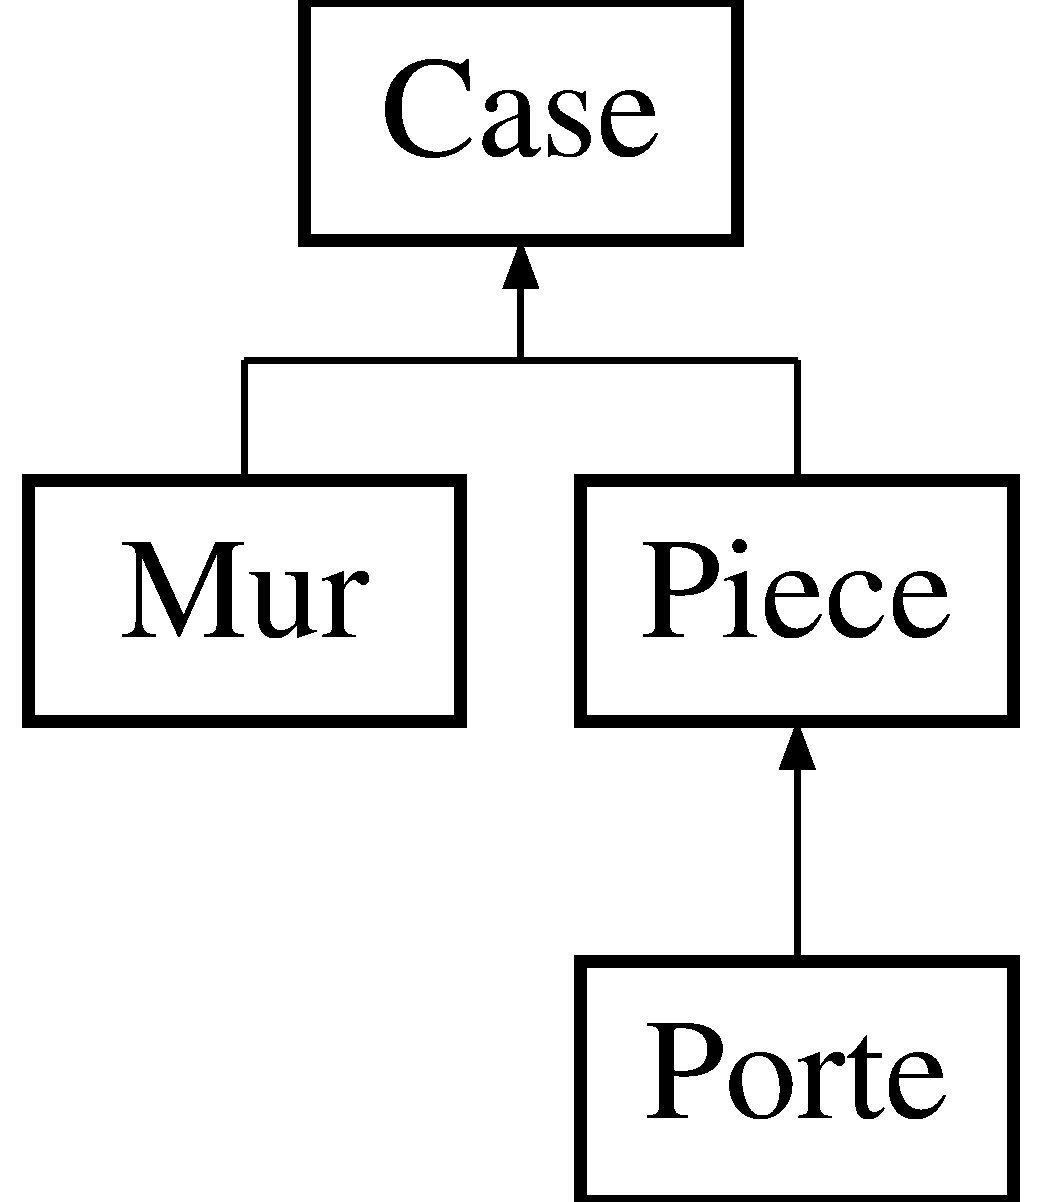
\includegraphics[height=3.000000cm]{classCase}
\end{center}
\end{figure}
\subsection*{\-Fonctions membres publiques}
\begin{DoxyCompactItemize}
\item 
\hypertarget{classCase_a14237e17aab1829965adab76b747db6c}{\hyperlink{classCase_a14237e17aab1829965adab76b747db6c}{\-Case} ()}\label{classCase_a14237e17aab1829965adab76b747db6c}

\begin{DoxyCompactList}\small\item\em \-Constructeur par defaut. \end{DoxyCompactList}\item 
\hyperlink{classCase_ad61be010b8d3cc841706c989c08aaaac}{\-Case} (int a, int b)
\begin{DoxyCompactList}\small\item\em \-Constructeur. \end{DoxyCompactList}\item 
bool \hyperlink{classCase_aba81e8660bf4009cc0ddee8e132bce49}{operator==} (\hyperlink{classCase}{\-Case} const \&c2)
\begin{DoxyCompactList}\small\item\em \-Operateur d'egalite. \end{DoxyCompactList}\item 
\hypertarget{classCase_ab004564aae3e15db0c7fd5dde0b4c379}{virtual \hyperlink{classCase_ab004564aae3e15db0c7fd5dde0b4c379}{$\sim$\-Case} ()}\label{classCase_ab004564aae3e15db0c7fd5dde0b4c379}

\begin{DoxyCompactList}\small\item\em \-Destructeur. \end{DoxyCompactList}\item 
\hypertarget{classCase_ad3faa1f96e315587b4fb70de225a8b80}{void {\bfseries afficher} ()}\label{classCase_ad3faa1f96e315587b4fb70de225a8b80}

\item 
virtual std\-::string \hyperlink{classCase_ad09ca1072f39bcacf06459fc03f026ae}{to\-String} ()
\begin{DoxyCompactList}\small\item\em \-Méthode qui retrourne une string repésentant la case du type\-: \mbox{[}x\mbox{]}\mbox{[}y\mbox{]}. \end{DoxyCompactList}\item 
virtual void \hyperlink{classCase_affe73b57a2c81e2f09dc5db45893db3c}{trouver\-Chemin} (int de, std\-::vector$<$ \hyperlink{classCase}{\-Case} $\ast$ $>$ \&res, \hyperlink{classPlateau}{\-Plateau} $\ast$p)
\begin{DoxyCompactList}\small\item\em \-Methode qui trouve tous les chemins possibles. \end{DoxyCompactList}\item 
virtual std\-::string \hyperlink{classCase_acdbbc0ad8422141cdbf2e647d1ba56e1}{action} ()
\begin{DoxyCompactList}\small\item\em \-Methode qui va réaliser l'action selon la case. \end{DoxyCompactList}\item 
std\-::pair$<$ int, int $>$ \hyperlink{classCase_ae6ce55820f949e5fae8dbeb62d298291}{point\-H\-G} (int taille\-Case, int ecart\-X, int ecart\-Y)
\begin{DoxyCompactList}\small\item\em \-Renvoie le point en haut à gauche de la case en fonction de l'affichage. \end{DoxyCompactList}\item 
std\-::pair$<$ int, int $>$ \hyperlink{classCase_a48b794ecbea4155843ce09f53e280237}{milieu} (int taille\-Case, std\-::pair$<$ int, int $>$ a)
\begin{DoxyCompactList}\small\item\em \-Renvoie le point permettant de mettre le pion au centre de la case. \end{DoxyCompactList}\item 
void \hyperlink{classCase_ad7cbf9289ac69b4e1c1f3fc20a6fa540}{colorier} (sf\-::\-Render\-Window \&window)
\begin{DoxyCompactList}\small\item\em \-Methode qui va colorier en bleu la case. \end{DoxyCompactList}\item 
virtual int \hyperlink{classCase_ab5580b919199dd2ec379672d3390bbff}{get\-X} ()
\begin{DoxyCompactList}\small\item\em \-Assesseur de x\-\_\-. \end{DoxyCompactList}\item 
virtual int \hyperlink{classCase_a824f612c5a660a1d55ac06931747c46d}{get\-Y} ()
\begin{DoxyCompactList}\small\item\em \-Assesseur de y\-\_\-. \end{DoxyCompactList}\item 
virtual int \hyperlink{classCase_a80ae0e9d1a9c575bee4c8a7b984deb59}{get\-Est\-Vide} ()
\begin{DoxyCompactList}\small\item\em \-Assesseur de est\-Vide. \end{DoxyCompactList}\item 
\hypertarget{classCase_a292e07394ff0a1c31ebf35940c91f29d}{virtual void \hyperlink{classCase_a292e07394ff0a1c31ebf35940c91f29d}{set\-Est\-Vide} (bool b)}\label{classCase_a292e07394ff0a1c31ebf35940c91f29d}

\begin{DoxyCompactList}\small\item\em \-Modificateur de est\-Vide. \end{DoxyCompactList}\end{DoxyCompactItemize}
\subsection*{\-Attributs protégés}
\begin{DoxyCompactItemize}
\item 
\hypertarget{classCase_a45ecd9780447322263846abde6b5dfb8}{int {\bfseries x\-\_\-}}\label{classCase_a45ecd9780447322263846abde6b5dfb8}

\item 
\hypertarget{classCase_a44d580d307f1bacd6e68fc1384afc296}{int {\bfseries y\-\_\-}}\label{classCase_a44d580d307f1bacd6e68fc1384afc296}

\item 
\hypertarget{classCase_a8a42e3989f79ab7f95635d59e7c20ba5}{bool {\bfseries est\-Vide}}\label{classCase_a8a42e3989f79ab7f95635d59e7c20ba5}

\item 
\hypertarget{classCase_a09b40766357ec483aa249103c35eaf81}{sf\-::\-Rectangle\-Shape $\ast$ {\bfseries rectangle}}\label{classCase_a09b40766357ec483aa249103c35eaf81}

\end{DoxyCompactItemize}
\subsection*{\-Attributs protégés statiques}
\begin{DoxyCompactItemize}
\item 
\hypertarget{classCase_a9263e52fca2d5567d0bb07d51bc7d302}{static const int {\bfseries taille\-\_\-} = 20}\label{classCase_a9263e52fca2d5567d0bb07d51bc7d302}

\end{DoxyCompactItemize}


\subsection{\-Description détaillée}
\hyperlink{classCase}{\-Case} est la classe représentant les cases du plateau. 

\-Une \hyperlink{classCase}{\-Case} est caractérisé par les informations suivantes \-: un x un y un bool estvide

\-Herite de \hyperlink{classCase}{\-Case}.

\begin{DoxyAuthor}{\-Auteur}
\-Olivia \-Bruce 

\-Cassandre \-Gloria 
\end{DoxyAuthor}
\begin{DoxyVersion}{\-Version}
1.\-0 
\end{DoxyVersion}


\subsection{\-Documentation des constructeurs et destructeur}
\hypertarget{classCase_ad61be010b8d3cc841706c989c08aaaac}{\index{\-Case@{\-Case}!\-Case@{\-Case}}
\index{\-Case@{\-Case}!Case@{\-Case}}
\subsubsection[{\-Case}]{\setlength{\rightskip}{0pt plus 5cm}{\bf \-Case\-::\-Case} (
\begin{DoxyParamCaption}
\item[{int}]{a, }
\item[{int}]{b}
\end{DoxyParamCaption}
)}}\label{classCase_ad61be010b8d3cc841706c989c08aaaac}


\-Constructeur. 


\begin{DoxyParams}{\-Paramètres}
{\em a} & ordonnee \\
\hline
{\em b} & abscisse \\
\hline
\end{DoxyParams}


\subsection{\-Documentation des fonctions membres}
\hypertarget{classCase_acdbbc0ad8422141cdbf2e647d1ba56e1}{\index{\-Case@{\-Case}!action@{action}}
\index{action@{action}!Case@{\-Case}}
\subsubsection[{action}]{\setlength{\rightskip}{0pt plus 5cm}std\-::string {\bf \-Case\-::action} (
\begin{DoxyParamCaption}
{}
\end{DoxyParamCaption}
)\hspace{0.3cm}{\ttfamily  \mbox{[}virtual\mbox{]}}}}\label{classCase_acdbbc0ad8422141cdbf2e647d1ba56e1}


\-Methode qui va réaliser l'action selon la case. 

\begin{DoxyReturn}{\-Renvoie}
une string vide ici 
\end{DoxyReturn}


\-Réimplémentée dans \hyperlink{classPorte_a71f6ed526931178c012e8653e609e0e7}{\-Porte}, \hyperlink{classPiece_ae2bbb51808f5d87be1761df503571e0d}{\-Piece}, et \hyperlink{classMur_a0fda0e8825c34a5f06d651e263bff058}{\-Mur}.

\hypertarget{classCase_ad7cbf9289ac69b4e1c1f3fc20a6fa540}{\index{\-Case@{\-Case}!colorier@{colorier}}
\index{colorier@{colorier}!Case@{\-Case}}
\subsubsection[{colorier}]{\setlength{\rightskip}{0pt plus 5cm}void {\bf \-Case\-::colorier} (
\begin{DoxyParamCaption}
\item[{sf\-::\-Render\-Window \&}]{window}
\end{DoxyParamCaption}
)}}\label{classCase_ad7cbf9289ac69b4e1c1f3fc20a6fa540}


\-Methode qui va colorier en bleu la case. 


\begin{DoxyParams}{\-Paramètres}
{\em window} & la fenetre qui va etre touchée \\
\hline
\end{DoxyParams}
\hypertarget{classCase_a80ae0e9d1a9c575bee4c8a7b984deb59}{\index{\-Case@{\-Case}!get\-Est\-Vide@{get\-Est\-Vide}}
\index{get\-Est\-Vide@{get\-Est\-Vide}!Case@{\-Case}}
\subsubsection[{get\-Est\-Vide}]{\setlength{\rightskip}{0pt plus 5cm}int {\bf \-Case\-::get\-Est\-Vide} (
\begin{DoxyParamCaption}
{}
\end{DoxyParamCaption}
)\hspace{0.3cm}{\ttfamily  \mbox{[}virtual\mbox{]}}}}\label{classCase_a80ae0e9d1a9c575bee4c8a7b984deb59}


\-Assesseur de est\-Vide. 

\begin{DoxyReturn}{\-Renvoie}
est\-Vide si la case estvide ou non 
\end{DoxyReturn}
\hypertarget{classCase_ab5580b919199dd2ec379672d3390bbff}{\index{\-Case@{\-Case}!get\-X@{get\-X}}
\index{get\-X@{get\-X}!Case@{\-Case}}
\subsubsection[{get\-X}]{\setlength{\rightskip}{0pt plus 5cm}int {\bf \-Case\-::get\-X} (
\begin{DoxyParamCaption}
{}
\end{DoxyParamCaption}
)\hspace{0.3cm}{\ttfamily  \mbox{[}virtual\mbox{]}}}}\label{classCase_ab5580b919199dd2ec379672d3390bbff}


\-Assesseur de x\-\_\-. 

\begin{DoxyReturn}{\-Renvoie}
x\-\_\- l'absisse de la case 
\end{DoxyReturn}
\hypertarget{classCase_a824f612c5a660a1d55ac06931747c46d}{\index{\-Case@{\-Case}!get\-Y@{get\-Y}}
\index{get\-Y@{get\-Y}!Case@{\-Case}}
\subsubsection[{get\-Y}]{\setlength{\rightskip}{0pt plus 5cm}int {\bf \-Case\-::get\-Y} (
\begin{DoxyParamCaption}
{}
\end{DoxyParamCaption}
)\hspace{0.3cm}{\ttfamily  \mbox{[}virtual\mbox{]}}}}\label{classCase_a824f612c5a660a1d55ac06931747c46d}


\-Assesseur de y\-\_\-. 

\begin{DoxyReturn}{\-Renvoie}
y\-\_\- l'ordonnee de la case 
\end{DoxyReturn}
\hypertarget{classCase_a48b794ecbea4155843ce09f53e280237}{\index{\-Case@{\-Case}!milieu@{milieu}}
\index{milieu@{milieu}!Case@{\-Case}}
\subsubsection[{milieu}]{\setlength{\rightskip}{0pt plus 5cm}pair$<$ int, int $>$ {\bf \-Case\-::milieu} (
\begin{DoxyParamCaption}
\item[{int}]{taille\-Case, }
\item[{std\-::pair$<$ int, int $>$}]{a}
\end{DoxyParamCaption}
)}}\label{classCase_a48b794ecbea4155843ce09f53e280237}


\-Renvoie le point permettant de mettre le pion au centre de la case. 

\begin{DoxyReturn}{\-Renvoie}
une pair d'int représentant l'endroit pour bien placer le pion 
\end{DoxyReturn}
\hypertarget{classCase_aba81e8660bf4009cc0ddee8e132bce49}{\index{\-Case@{\-Case}!operator==@{operator==}}
\index{operator==@{operator==}!Case@{\-Case}}
\subsubsection[{operator==}]{\setlength{\rightskip}{0pt plus 5cm}bool \-Case\-::operator== (
\begin{DoxyParamCaption}
\item[{{\bf \-Case} const \&}]{c2}
\end{DoxyParamCaption}
)}}\label{classCase_aba81e8660bf4009cc0ddee8e132bce49}


\-Operateur d'egalite. 


\begin{DoxyParams}{\-Paramètres}
{\em c2} & la seconde case \\
\hline
\end{DoxyParams}
\hypertarget{classCase_ae6ce55820f949e5fae8dbeb62d298291}{\index{\-Case@{\-Case}!point\-H\-G@{point\-H\-G}}
\index{point\-H\-G@{point\-H\-G}!Case@{\-Case}}
\subsubsection[{point\-H\-G}]{\setlength{\rightskip}{0pt plus 5cm}pair$<$ int, int $>$ {\bf \-Case\-::point\-H\-G} (
\begin{DoxyParamCaption}
\item[{int}]{taille\-Case, }
\item[{int}]{ecart\-X, }
\item[{int}]{ecart\-Y}
\end{DoxyParamCaption}
)}}\label{classCase_ae6ce55820f949e5fae8dbeb62d298291}


\-Renvoie le point en haut à gauche de la case en fonction de l'affichage. 

\begin{DoxyReturn}{\-Renvoie}
une pair d'int représentant le point en hautà gauche 
\end{DoxyReturn}
\hypertarget{classCase_ad09ca1072f39bcacf06459fc03f026ae}{\index{\-Case@{\-Case}!to\-String@{to\-String}}
\index{to\-String@{to\-String}!Case@{\-Case}}
\subsubsection[{to\-String}]{\setlength{\rightskip}{0pt plus 5cm}std\-::string {\bf \-Case\-::to\-String} (
\begin{DoxyParamCaption}
{}
\end{DoxyParamCaption}
)\hspace{0.3cm}{\ttfamily  \mbox{[}virtual\mbox{]}}}}\label{classCase_ad09ca1072f39bcacf06459fc03f026ae}


\-Méthode qui retrourne une string repésentant la case du type\-: \mbox{[}x\mbox{]}\mbox{[}y\mbox{]}. 

\begin{DoxyReturn}{\-Renvoie}
res l'emplacement de la case 
\end{DoxyReturn}


\-Réimplémentée dans \hyperlink{classPorte_ace3891879a69f2d29ade65d71d869377}{\-Porte}, \hyperlink{classPiece_ae18523c400cb72a50bb1293d27cd1432}{\-Piece}, et \hyperlink{classMur_a8d319947a0158801579dc5f1f8568281}{\-Mur}.

\hypertarget{classCase_affe73b57a2c81e2f09dc5db45893db3c}{\index{\-Case@{\-Case}!trouver\-Chemin@{trouver\-Chemin}}
\index{trouver\-Chemin@{trouver\-Chemin}!Case@{\-Case}}
\subsubsection[{trouver\-Chemin}]{\setlength{\rightskip}{0pt plus 5cm}void {\bf \-Case\-::trouver\-Chemin} (
\begin{DoxyParamCaption}
\item[{int}]{de, }
\item[{std\-::vector$<$ {\bf \-Case} $\ast$ $>$ \&}]{res, }
\item[{{\bf \-Plateau} $\ast$}]{p}
\end{DoxyParamCaption}
)\hspace{0.3cm}{\ttfamily  \mbox{[}virtual\mbox{]}}}}\label{classCase_affe73b57a2c81e2f09dc5db45893db3c}


\-Methode qui trouve tous les chemins possibles. 


\begin{DoxyParams}{\-Paramètres}
{\em de} & le nombre a parcourir \\
\hline
{\em res} & le vetor des chemins \\
\hline
{\em p} & le plateau \\
\hline
\end{DoxyParams}


\-La documentation de cette classe a été générée à partir des fichiers suivants \-:\begin{DoxyCompactItemize}
\item 
\-Case.\-h\item 
\-Case.\-cpp\end{DoxyCompactItemize}

\hypertarget{classDonnees}{\section{\-Référence de la classe \-Donnees}
\label{classDonnees}\index{\-Donnees@{\-Donnees}}
}
\subsection*{\-Fonctions membres publiques}
\begin{DoxyCompactItemize}
\item 
\hypertarget{classDonnees_af238721bd5caba48da9d7531f1156f18}{\hyperlink{classCarte}{\-Carte} $\ast$ {\bfseries get\-Carte} (int indice)}\label{classDonnees_af238721bd5caba48da9d7531f1156f18}

\item 
vector$<$ \hyperlink{classCarte}{\-Carte} $\ast$ $>$ \hyperlink{classDonnees_a574a33fb002aa10927bd97c39b84839b}{init\-Carte\-Mystere} (vector$<$ int $>$ \&vec)
\begin{DoxyCompactList}\small\item\em \-Retourne les cartes mysteres. \end{DoxyCompactList}\item 
vector$<$ \hyperlink{classJoueur}{\-Joueur} $>$ \hyperlink{classDonnees_a85ad060f19a3f27d07699495b8be4fe0}{init\-Joueur} (int n)
\begin{DoxyCompactList}\small\item\em \-Va renvoyer un n nombre de joueur avec des persos aléatoires. \end{DoxyCompactList}\item 
\hypertarget{classDonnees_a1f7c9ce96432a2cb384d4f1fb22c59f7}{void {\bfseries positionner\-Perso} (\hyperlink{classPlateau}{\-Plateau} $\ast$p)}\label{classDonnees_a1f7c9ce96432a2cb384d4f1fb22c59f7}

\item 
vector$<$ \hyperlink{classCarte}{\-Carte} $\ast$ $>$ \hyperlink{classDonnees_ae61912de3804ec0a33be8a3168a41b72}{distribuer\-Carte} (vector$<$ \hyperlink{classJoueur}{\-Joueur} $>$ \&les\-Joueurs)
\begin{DoxyCompactList}\small\item\em \-Methodes qui va distribuer les cartes aux joueurs. \end{DoxyCompactList}\end{DoxyCompactItemize}


\subsection{\-Documentation des fonctions membres}
\hypertarget{classDonnees_ae61912de3804ec0a33be8a3168a41b72}{\index{\-Donnees@{\-Donnees}!distribuer\-Carte@{distribuer\-Carte}}
\index{distribuer\-Carte@{distribuer\-Carte}!Donnees@{\-Donnees}}
\subsubsection[{distribuer\-Carte}]{\setlength{\rightskip}{0pt plus 5cm}vector$<$ {\bf \-Carte} $\ast$ $>$ {\bf \-Donnees\-::distribuer\-Carte} (
\begin{DoxyParamCaption}
\item[{vector$<$ {\bf \-Joueur} $>$ \&}]{les\-Joueurs}
\end{DoxyParamCaption}
)}}\label{classDonnees_ae61912de3804ec0a33be8a3168a41b72}


\-Methodes qui va distribuer les cartes aux joueurs. 

\hypertarget{classDonnees_a574a33fb002aa10927bd97c39b84839b}{\index{\-Donnees@{\-Donnees}!init\-Carte\-Mystere@{init\-Carte\-Mystere}}
\index{init\-Carte\-Mystere@{init\-Carte\-Mystere}!Donnees@{\-Donnees}}
\subsubsection[{init\-Carte\-Mystere}]{\setlength{\rightskip}{0pt plus 5cm}vector$<$ {\bf \-Carte} $\ast$ $>$ {\bf \-Donnees\-::init\-Carte\-Mystere} (
\begin{DoxyParamCaption}
\item[{vector$<$ int $>$ \&}]{temoin}
\end{DoxyParamCaption}
)}}\label{classDonnees_a574a33fb002aa10927bd97c39b84839b}


\-Retourne les cartes mysteres. 

\hypertarget{classDonnees_a85ad060f19a3f27d07699495b8be4fe0}{\index{\-Donnees@{\-Donnees}!init\-Joueur@{init\-Joueur}}
\index{init\-Joueur@{init\-Joueur}!Donnees@{\-Donnees}}
\subsubsection[{init\-Joueur}]{\setlength{\rightskip}{0pt plus 5cm}vector$<$ {\bf \-Joueur} $>$ {\bf \-Donnees\-::init\-Joueur} (
\begin{DoxyParamCaption}
\item[{int}]{n}
\end{DoxyParamCaption}
)}}\label{classDonnees_a85ad060f19a3f27d07699495b8be4fe0}


\-Va renvoyer un n nombre de joueur avec des persos aléatoires. 



\-La documentation de cette classe a été générée à partir des fichiers suivants \-:\begin{DoxyCompactItemize}
\item 
\-Donnees.\-h\item 
\-Donnees.\-cpp\end{DoxyCompactItemize}

\hypertarget{classDonneesJeu}{\section{\-Référence de la classe \-Donnees\-Jeu}
\label{classDonneesJeu}\index{\-Donnees\-Jeu@{\-Donnees\-Jeu}}
}


\hyperlink{classDonneesJeu}{\-Donnees\-Jeu} est la classe représentant les donnees avant le debut du jeu.  




{\ttfamily \#include $<$\-Donnees\-Jeu.\-h$>$}

\subsection*{\-Fonctions membres publiques}
\begin{DoxyCompactItemize}
\item 
\hypertarget{classDonneesJeu_a8481b1b72ec382f7c5b34d564bd6a39c}{{\bfseries \-Donnees\-Jeu} (\hyperlink{classDonnees}{\-Donnees} $\ast$d)}\label{classDonneesJeu_a8481b1b72ec382f7c5b34d564bd6a39c}

\item 
int \hyperlink{classDonneesJeu_a39169eecf0e197ccf5677c7a1602a172}{lancer\-De} ()
\begin{DoxyCompactList}\small\item\em \-Methoque qui prend un nombre aleatoire entre 2 et 12. \end{DoxyCompactList}\item 
\hypertarget{classDonneesJeu_aa8f22aa69faeb3e54d76a5aaa3d4444f}{void \hyperlink{classDonneesJeu_aa8f22aa69faeb3e54d76a5aaa3d4444f}{preparer\-Partie} (\hyperlink{classPlateau}{\-Plateau} $\ast$plateau)}\label{classDonneesJeu_aa8f22aa69faeb3e54d76a5aaa3d4444f}

\begin{DoxyCompactList}\small\item\em \-Methode qui va preparer la partie. \end{DoxyCompactList}\item 
void \hyperlink{classDonneesJeu_ae443a7d34f88fe863914746b6e1fefd9}{changer\-Joueur} ()
\begin{DoxyCompactList}\small\item\em \-Methode qui met a jour le joueur \-Courant. \end{DoxyCompactList}\item 
void \hyperlink{classDonneesJeu_a0329e6f5906aca754330ee17d7b4ab56}{accuser} (std\-::string arme, std\-::string perso, std\-::string lieu)
\begin{DoxyCompactList}\small\item\em \-Methode qui va permettre au joueur courant d'accuser. \end{DoxyCompactList}\item 
std\-::string \hyperlink{classDonneesJeu_a5db87f4ec8d3d5b790ec58b6b17931e1}{soupconner} (std\-::string arme, std\-::string perso, std\-::string lieu)
\begin{DoxyCompactList}\small\item\em \-Methode qui va permettre au joueur courant de soupconner. \end{DoxyCompactList}\item 
bool \hyperlink{classDonneesJeu_a7d47cf2b384712fd2aca3494fc5e23b8}{get\-Partie\-Fini} ()
\begin{DoxyCompactList}\small\item\em \-Methode qui retourne si la partie est finie. \end{DoxyCompactList}\item 
void \hyperlink{classDonneesJeu_a97ab9601b004cb1ffd4365db0f90e479}{set\-Partie\-Fini} (bool parti)
\begin{DoxyCompactList}\small\item\em \-Methode qui met a jour l'etat de la partie. \end{DoxyCompactList}\item 
\hyperlink{classJoueur}{\-Joueur} $\ast$ \hyperlink{classDonneesJeu_a5c71130d171fbd79f39f90d1ab96d82c}{get\-Joueur\-Courant} ()
\begin{DoxyCompactList}\small\item\em \-Methode qui retourne le joueur courant. \end{DoxyCompactList}\item 
\hyperlink{classJoueur}{\-Joueur} $\ast$ \hyperlink{classDonneesJeu_a94ac64e9b0a6ec3e10a2589bb90830e4}{get\-Joueur\-At} (int i)
\begin{DoxyCompactList}\small\item\em \-Methode qui retourne le joueur à la position. \end{DoxyCompactList}\item 
int \hyperlink{classDonneesJeu_a9d66541ae27e731bcd4fca1a82b8c94f}{get\-De} ()
\begin{DoxyCompactList}\small\item\em \-Methode qui retourne le de. \end{DoxyCompactList}\item 
\hyperlink{classJoueur}{\-Joueur} $\ast$ \hyperlink{classDonneesJeu_a1f9959f0eae2138deb88422671c6a1f2}{get\-Gagnant} ()
\begin{DoxyCompactList}\small\item\em \-Methode qui retourne le joueur gagnant. \end{DoxyCompactList}\item 
void \hyperlink{classDonneesJeu_a2b7a86ddb0732fe79afa5f4ad71af9d2}{set\-Gagnant} (\hyperlink{classJoueur}{\-Joueur} $\ast$j)
\begin{DoxyCompactList}\small\item\em \-Methode qui met a jour le joueur gagnant. \end{DoxyCompactList}\item 
void \hyperlink{classDonneesJeu_a1da6b561395378b12e3331cb61d1a6ad}{set\-Nb\-Joueur} (int nb)
\begin{DoxyCompactList}\small\item\em \-Methode qui met a jour le nombre de joueur. \end{DoxyCompactList}\item 
int \hyperlink{classDonneesJeu_a7b698e7aea2dd33cf744b5532c59eb1f}{get\-Nb\-Joueur} ()
\begin{DoxyCompactList}\small\item\em \-Methode qui get le nombre de joueur. \end{DoxyCompactList}\end{DoxyCompactItemize}


\subsection{\-Description détaillée}
\hyperlink{classDonneesJeu}{\-Donnees\-Jeu} est la classe représentant les donnees avant le debut du jeu. 

\-Une \hyperlink{classDonneesJeu}{\-Donnees\-Jeu} est caractérisé par les informations suivantes \-: des donnees un pointeur vers joueur gagnant nul au depart un tableau de carte$\ast$ mysteres un booleen disant si la partie est fini un joueur\-Courant un nombre de joueur

\begin{DoxyAuthor}{\-Auteur}
\-Olivia \-Bruce 

\-Cassandre \-Gloria 
\end{DoxyAuthor}
\begin{DoxyVersion}{\-Version}
1.\-0 
\end{DoxyVersion}


\subsection{\-Documentation des fonctions membres}
\hypertarget{classDonneesJeu_a0329e6f5906aca754330ee17d7b4ab56}{\index{\-Donnees\-Jeu@{\-Donnees\-Jeu}!accuser@{accuser}}
\index{accuser@{accuser}!DonneesJeu@{\-Donnees\-Jeu}}
\subsubsection[{accuser}]{\setlength{\rightskip}{0pt plus 5cm}void {\bf \-Donnees\-Jeu\-::accuser} (
\begin{DoxyParamCaption}
\item[{std\-::string}]{arme, }
\item[{std\-::string}]{perso, }
\item[{std\-::string}]{lieu}
\end{DoxyParamCaption}
)}}\label{classDonneesJeu_a0329e6f5906aca754330ee17d7b4ab56}


\-Methode qui va permettre au joueur courant d'accuser. 


\begin{DoxyParams}{\-Paramètres}
{\em arme} & l'arme du crime \\
\hline
{\em lieu} & la piece ou est le joueur \\
\hline
{\em perso} & le criminelle \\
\hline
\end{DoxyParams}
\hypertarget{classDonneesJeu_ae443a7d34f88fe863914746b6e1fefd9}{\index{\-Donnees\-Jeu@{\-Donnees\-Jeu}!changer\-Joueur@{changer\-Joueur}}
\index{changer\-Joueur@{changer\-Joueur}!DonneesJeu@{\-Donnees\-Jeu}}
\subsubsection[{changer\-Joueur}]{\setlength{\rightskip}{0pt plus 5cm}void {\bf \-Donnees\-Jeu\-::changer\-Joueur} (
\begin{DoxyParamCaption}
{}
\end{DoxyParamCaption}
)}}\label{classDonneesJeu_ae443a7d34f88fe863914746b6e1fefd9}


\-Methode qui met a jour le joueur \-Courant. 


\begin{DoxyParams}{\-Paramètres}
{\em joueur\-Courant} & le joueur corant dans le tab\-Joueur\-\_\- \\
\hline
\end{DoxyParams}
\hypertarget{classDonneesJeu_a9d66541ae27e731bcd4fca1a82b8c94f}{\index{\-Donnees\-Jeu@{\-Donnees\-Jeu}!get\-De@{get\-De}}
\index{get\-De@{get\-De}!DonneesJeu@{\-Donnees\-Jeu}}
\subsubsection[{get\-De}]{\setlength{\rightskip}{0pt plus 5cm}int {\bf \-Donnees\-Jeu\-::get\-De} (
\begin{DoxyParamCaption}
{}
\end{DoxyParamCaption}
)}}\label{classDonneesJeu_a9d66541ae27e731bcd4fca1a82b8c94f}


\-Methode qui retourne le de. 

\begin{DoxyReturn}{\-Renvoie}
le dé 
\end{DoxyReturn}
\hypertarget{classDonneesJeu_a1f9959f0eae2138deb88422671c6a1f2}{\index{\-Donnees\-Jeu@{\-Donnees\-Jeu}!get\-Gagnant@{get\-Gagnant}}
\index{get\-Gagnant@{get\-Gagnant}!DonneesJeu@{\-Donnees\-Jeu}}
\subsubsection[{get\-Gagnant}]{\setlength{\rightskip}{0pt plus 5cm}{\bf \-Joueur} $\ast$ {\bf \-Donnees\-Jeu\-::get\-Gagnant} (
\begin{DoxyParamCaption}
{}
\end{DoxyParamCaption}
)}}\label{classDonneesJeu_a1f9959f0eae2138deb88422671c6a1f2}


\-Methode qui retourne le joueur gagnant. 

\begin{DoxyReturn}{\-Renvoie}
gagnant 
\end{DoxyReturn}
\hypertarget{classDonneesJeu_a94ac64e9b0a6ec3e10a2589bb90830e4}{\index{\-Donnees\-Jeu@{\-Donnees\-Jeu}!get\-Joueur\-At@{get\-Joueur\-At}}
\index{get\-Joueur\-At@{get\-Joueur\-At}!DonneesJeu@{\-Donnees\-Jeu}}
\subsubsection[{get\-Joueur\-At}]{\setlength{\rightskip}{0pt plus 5cm}{\bf \-Joueur} $\ast$ {\bf \-Donnees\-Jeu\-::get\-Joueur\-At} (
\begin{DoxyParamCaption}
\item[{int}]{i}
\end{DoxyParamCaption}
)}}\label{classDonneesJeu_a94ac64e9b0a6ec3e10a2589bb90830e4}


\-Methode qui retourne le joueur à la position. 

\begin{DoxyReturn}{\-Renvoie}
joueur\-Courant 
\end{DoxyReturn}
\hypertarget{classDonneesJeu_a5c71130d171fbd79f39f90d1ab96d82c}{\index{\-Donnees\-Jeu@{\-Donnees\-Jeu}!get\-Joueur\-Courant@{get\-Joueur\-Courant}}
\index{get\-Joueur\-Courant@{get\-Joueur\-Courant}!DonneesJeu@{\-Donnees\-Jeu}}
\subsubsection[{get\-Joueur\-Courant}]{\setlength{\rightskip}{0pt plus 5cm}{\bf \-Joueur} $\ast$ {\bf \-Donnees\-Jeu\-::get\-Joueur\-Courant} (
\begin{DoxyParamCaption}
{}
\end{DoxyParamCaption}
)}}\label{classDonneesJeu_a5c71130d171fbd79f39f90d1ab96d82c}


\-Methode qui retourne le joueur courant. 

\begin{DoxyReturn}{\-Renvoie}
joueur\-Courant 
\end{DoxyReturn}
\hypertarget{classDonneesJeu_a7b698e7aea2dd33cf744b5532c59eb1f}{\index{\-Donnees\-Jeu@{\-Donnees\-Jeu}!get\-Nb\-Joueur@{get\-Nb\-Joueur}}
\index{get\-Nb\-Joueur@{get\-Nb\-Joueur}!DonneesJeu@{\-Donnees\-Jeu}}
\subsubsection[{get\-Nb\-Joueur}]{\setlength{\rightskip}{0pt plus 5cm}int {\bf \-Donnees\-Jeu\-::get\-Nb\-Joueur} (
\begin{DoxyParamCaption}
{}
\end{DoxyParamCaption}
)}}\label{classDonneesJeu_a7b698e7aea2dd33cf744b5532c59eb1f}


\-Methode qui get le nombre de joueur. 


\begin{DoxyParams}{\-Paramètres}
{\em joueur\-Courant} & le joueur corant dans le tab\-Joueur\-\_\- \\
\hline
\end{DoxyParams}
\hypertarget{classDonneesJeu_a7d47cf2b384712fd2aca3494fc5e23b8}{\index{\-Donnees\-Jeu@{\-Donnees\-Jeu}!get\-Partie\-Fini@{get\-Partie\-Fini}}
\index{get\-Partie\-Fini@{get\-Partie\-Fini}!DonneesJeu@{\-Donnees\-Jeu}}
\subsubsection[{get\-Partie\-Fini}]{\setlength{\rightskip}{0pt plus 5cm}bool {\bf \-Donnees\-Jeu\-::get\-Partie\-Fini} (
\begin{DoxyParamCaption}
{}
\end{DoxyParamCaption}
)}}\label{classDonneesJeu_a7d47cf2b384712fd2aca3494fc5e23b8}


\-Methode qui retourne si la partie est finie. 

\begin{DoxyReturn}{\-Renvoie}
partie\-Fini\-\_\- true si fini et false si non fini 
\end{DoxyReturn}
\hypertarget{classDonneesJeu_a39169eecf0e197ccf5677c7a1602a172}{\index{\-Donnees\-Jeu@{\-Donnees\-Jeu}!lancer\-De@{lancer\-De}}
\index{lancer\-De@{lancer\-De}!DonneesJeu@{\-Donnees\-Jeu}}
\subsubsection[{lancer\-De}]{\setlength{\rightskip}{0pt plus 5cm}int {\bf \-Donnees\-Jeu\-::lancer\-De} (
\begin{DoxyParamCaption}
{}
\end{DoxyParamCaption}
)}}\label{classDonneesJeu_a39169eecf0e197ccf5677c7a1602a172}


\-Methoque qui prend un nombre aleatoire entre 2 et 12. 

\begin{DoxyReturn}{\-Renvoie}
rand un random entre 2 et 12 
\end{DoxyReturn}
\hypertarget{classDonneesJeu_a2b7a86ddb0732fe79afa5f4ad71af9d2}{\index{\-Donnees\-Jeu@{\-Donnees\-Jeu}!set\-Gagnant@{set\-Gagnant}}
\index{set\-Gagnant@{set\-Gagnant}!DonneesJeu@{\-Donnees\-Jeu}}
\subsubsection[{set\-Gagnant}]{\setlength{\rightskip}{0pt plus 5cm}void {\bf \-Donnees\-Jeu\-::set\-Gagnant} (
\begin{DoxyParamCaption}
\item[{{\bf \-Joueur} $\ast$}]{j}
\end{DoxyParamCaption}
)}}\label{classDonneesJeu_a2b7a86ddb0732fe79afa5f4ad71af9d2}


\-Methode qui met a jour le joueur gagnant. 


\begin{DoxyParams}{\-Paramètres}
{\em joueur\-Courant} & le joueur corant dans le tab\-Joueur\-\_\- \\
\hline
\end{DoxyParams}
\hypertarget{classDonneesJeu_a1da6b561395378b12e3331cb61d1a6ad}{\index{\-Donnees\-Jeu@{\-Donnees\-Jeu}!set\-Nb\-Joueur@{set\-Nb\-Joueur}}
\index{set\-Nb\-Joueur@{set\-Nb\-Joueur}!DonneesJeu@{\-Donnees\-Jeu}}
\subsubsection[{set\-Nb\-Joueur}]{\setlength{\rightskip}{0pt plus 5cm}void {\bf \-Donnees\-Jeu\-::set\-Nb\-Joueur} (
\begin{DoxyParamCaption}
\item[{int}]{nb}
\end{DoxyParamCaption}
)}}\label{classDonneesJeu_a1da6b561395378b12e3331cb61d1a6ad}


\-Methode qui met a jour le nombre de joueur. 


\begin{DoxyParams}{\-Paramètres}
{\em joueur\-Courant} & le joueur corant dans le tab\-Joueur\-\_\- \\
\hline
\end{DoxyParams}
\hypertarget{classDonneesJeu_a97ab9601b004cb1ffd4365db0f90e479}{\index{\-Donnees\-Jeu@{\-Donnees\-Jeu}!set\-Partie\-Fini@{set\-Partie\-Fini}}
\index{set\-Partie\-Fini@{set\-Partie\-Fini}!DonneesJeu@{\-Donnees\-Jeu}}
\subsubsection[{set\-Partie\-Fini}]{\setlength{\rightskip}{0pt plus 5cm}void {\bf \-Donnees\-Jeu\-::set\-Partie\-Fini} (
\begin{DoxyParamCaption}
\item[{bool}]{parti}
\end{DoxyParamCaption}
)}}\label{classDonneesJeu_a97ab9601b004cb1ffd4365db0f90e479}


\-Methode qui met a jour l'etat de la partie. 


\begin{DoxyParams}{\-Paramètres}
{\em parti} & qui est un boolean true si fini et false si non fini \\
\hline
\end{DoxyParams}
\hypertarget{classDonneesJeu_a5db87f4ec8d3d5b790ec58b6b17931e1}{\index{\-Donnees\-Jeu@{\-Donnees\-Jeu}!soupconner@{soupconner}}
\index{soupconner@{soupconner}!DonneesJeu@{\-Donnees\-Jeu}}
\subsubsection[{soupconner}]{\setlength{\rightskip}{0pt plus 5cm}std\-::string {\bf \-Donnees\-Jeu\-::soupconner} (
\begin{DoxyParamCaption}
\item[{std\-::string}]{arme, }
\item[{std\-::string}]{perso, }
\item[{std\-::string}]{lieu}
\end{DoxyParamCaption}
)}}\label{classDonneesJeu_a5db87f4ec8d3d5b790ec58b6b17931e1}


\-Methode qui va permettre au joueur courant de soupconner. 


\begin{DoxyParams}{\-Paramètres}
{\em arme} & l'arme du crime \\
\hline
{\em lieu} & la piece ou est le joueur \\
\hline
{\em perso} & le criminelle \\
\hline
\end{DoxyParams}
\begin{DoxyReturn}{\-Renvoie}
cheminres le chemin contrant le soupcon 
\end{DoxyReturn}


\-La documentation de cette classe a été générée à partir des fichiers suivants \-:\begin{DoxyCompactItemize}
\item 
\-Donnees\-Jeu.\-h\item 
\-Donnees\-Jeu.\-cpp\end{DoxyCompactItemize}

\hypertarget{classEcran}{\section{\-Référence de la classe \-Ecran}
\label{classEcran}\index{\-Ecran@{\-Ecran}}
}


\hyperlink{classEcran}{\-Ecran} est la classe abstraite représentant les ecrans.  




{\ttfamily \#include $<$\-Ecran.\-h$>$}

\-Graphe d'héritage de \-Ecran\-:\begin{figure}[H]
\begin{center}
\leavevmode
\includegraphics[height=1.435897cm]{classEcran}
\end{center}
\end{figure}
\subsection*{\-Fonctions membres publiques}
\begin{DoxyCompactItemize}
\item 
\hypertarget{classEcran_a2b1ad69e95ff2b6fb1a411b3645922e0}{virtual void {\bfseries afficher} (sf\-::\-Render\-Window \&fenetre)=0}\label{classEcran_a2b1ad69e95ff2b6fb1a411b3645922e0}

\item 
\hypertarget{classEcran_a03b54d987a5f17eab6463a3b84ef0ba4}{virtual void {\bfseries update} (sf\-::\-Event event)=0}\label{classEcran_a03b54d987a5f17eab6463a3b84ef0ba4}

\end{DoxyCompactItemize}


\subsection{\-Description détaillée}
\hyperlink{classEcran}{\-Ecran} est la classe abstraite représentant les ecrans. 

\begin{DoxyAuthor}{\-Auteur}
\-Olivia \-Bruce 

\-Cassandre \-Gloria 
\end{DoxyAuthor}
\begin{DoxyVersion}{\-Version}
1.\-0 
\end{DoxyVersion}


\-La documentation de cette classe a été générée à partir du fichier suivant \-:\begin{DoxyCompactItemize}
\item 
\-Ecran.\-h\end{DoxyCompactItemize}

\hypertarget{classEcranAccueil}{\section{\-Référence de la classe \-Ecran\-Accueil}
\label{classEcranAccueil}\index{\-Ecran\-Accueil@{\-Ecran\-Accueil}}
}


\hyperlink{classEcranAccueil}{\-Ecran\-Accueil} est la classe représentant l'ecran d'accueil du jeu.  




{\ttfamily \#include $<$\-Ecran\-Accueil.\-h$>$}

\-Graphe d'héritage de \-Ecran\-Accueil\-:\begin{figure}[H]
\begin{center}
\leavevmode
\includegraphics[height=2.000000cm]{classEcranAccueil}
\end{center}
\end{figure}
\subsection*{\-Fonctions membres publiques}
\begin{DoxyCompactItemize}
\item 
\hypertarget{classEcranAccueil_a53449fe44e756cbfe0d19c372fab9783}{\hyperlink{classEcranAccueil_a53449fe44e756cbfe0d19c372fab9783}{\-Ecran\-Accueil} (\hyperlink{classManagerEcran}{\-Manager\-Ecran} $\ast$manager)}\label{classEcranAccueil_a53449fe44e756cbfe0d19c372fab9783}

\begin{DoxyCompactList}\small\item\em \-Constructeur. \end{DoxyCompactList}\item 
void \hyperlink{classEcranAccueil_acc1f211002209380daa8d13f5664c118}{afficher} (sf\-::\-Render\-Window \&fenetre)
\begin{DoxyCompactList}\small\item\em \-Methode qui va afficher l'ecran tel qu'il est. \end{DoxyCompactList}\item 
void \hyperlink{classEcranAccueil_ac03953623402740bab58ab7fbb54fc3a}{update} (sf\-::\-Event event)
\begin{DoxyCompactList}\small\item\em \-Methode qui permet le changement d'ecran en fonction des evenements. \end{DoxyCompactList}\end{DoxyCompactItemize}


\subsection{\-Description détaillée}
\hyperlink{classEcranAccueil}{\-Ecran\-Accueil} est la classe représentant l'ecran d'accueil du jeu. 

\-Il est caractérisé par les informations suivantes \-: deux boutons une image un manager permettant de changer d'ecran

\begin{DoxyAuthor}{\-Auteur}
\-Olivia \-Bruce 

\-Cassandre \-Gloria 
\end{DoxyAuthor}
\begin{DoxyVersion}{\-Version}
1.\-0 
\end{DoxyVersion}


\subsection{\-Documentation des fonctions membres}
\hypertarget{classEcranAccueil_acc1f211002209380daa8d13f5664c118}{\index{\-Ecran\-Accueil@{\-Ecran\-Accueil}!afficher@{afficher}}
\index{afficher@{afficher}!EcranAccueil@{\-Ecran\-Accueil}}
\subsubsection[{afficher}]{\setlength{\rightskip}{0pt plus 5cm}void {\bf \-Ecran\-Accueil\-::afficher} (
\begin{DoxyParamCaption}
\item[{sf\-::\-Render\-Window \&}]{fenetre}
\end{DoxyParamCaption}
)\hspace{0.3cm}{\ttfamily  \mbox{[}virtual\mbox{]}}}}\label{classEcranAccueil_acc1f211002209380daa8d13f5664c118}


\-Methode qui va afficher l'ecran tel qu'il est. 


\begin{DoxyParams}{\-Paramètres}
{\em fenetre} & la fenetre sur laquelle on va appliquer les changementd \\
\hline
\end{DoxyParams}


\-Implémente \hyperlink{classEcran}{\-Ecran}.

\hypertarget{classEcranAccueil_ac03953623402740bab58ab7fbb54fc3a}{\index{\-Ecran\-Accueil@{\-Ecran\-Accueil}!update@{update}}
\index{update@{update}!EcranAccueil@{\-Ecran\-Accueil}}
\subsubsection[{update}]{\setlength{\rightskip}{0pt plus 5cm}void {\bf \-Ecran\-Accueil\-::update} (
\begin{DoxyParamCaption}
\item[{sf\-::\-Event}]{event}
\end{DoxyParamCaption}
)\hspace{0.3cm}{\ttfamily  \mbox{[}virtual\mbox{]}}}}\label{classEcranAccueil_ac03953623402740bab58ab7fbb54fc3a}


\-Methode qui permet le changement d'ecran en fonction des evenements. 


\begin{DoxyParams}{\-Paramètres}
{\em event} & un evenement envoyé par les classes superieurs \\
\hline
\end{DoxyParams}


\-Implémente \hyperlink{classEcran}{\-Ecran}.



\-La documentation de cette classe a été générée à partir des fichiers suivants \-:\begin{DoxyCompactItemize}
\item 
\-Ecran\-Accueil.\-h\item 
\-Ecran\-Accueil.\-cpp\end{DoxyCompactItemize}

\hypertarget{classEcranConfiguration}{\section{\-Référence de la classe \-Ecran\-Configuration}
\label{classEcranConfiguration}\index{\-Ecran\-Configuration@{\-Ecran\-Configuration}}
}


\hyperlink{classEcranAccueil}{\-Ecran\-Accueil} est la classe représentant l'ecran permettant de choisir le nombre de joueur.  




{\ttfamily \#include $<$\-Ecran\-Configuration.\-h$>$}

\-Graphe d'héritage de \-Ecran\-Configuration\-:\begin{figure}[H]
\begin{center}
\leavevmode
\includegraphics[height=2.000000cm]{classEcranConfiguration}
\end{center}
\end{figure}
\subsection*{\-Fonctions membres publiques}
\begin{DoxyCompactItemize}
\item 
\hypertarget{classEcranConfiguration_a40ba51dbd89594164d32ba0dbff817f2}{\hyperlink{classEcranConfiguration_a40ba51dbd89594164d32ba0dbff817f2}{\-Ecran\-Configuration} (\hyperlink{classManagerEcran}{\-Manager\-Ecran} $\ast$manager)}\label{classEcranConfiguration_a40ba51dbd89594164d32ba0dbff817f2}

\begin{DoxyCompactList}\small\item\em \-Constructeur. \end{DoxyCompactList}\item 
\hypertarget{classEcranConfiguration_aa65dbd2aca4c0b3853aea5eb8c92b98f}{virtual void {\bfseries creer\-Partie} ()}\label{classEcranConfiguration_aa65dbd2aca4c0b3853aea5eb8c92b98f}

\item 
void \hyperlink{classEcranConfiguration_ab1a7fd161795e7dd28e359f5b8bb25f7}{afficher} (sf\-::\-Render\-Window \&fenetre)
\begin{DoxyCompactList}\small\item\em \-Fonction afficher. \end{DoxyCompactList}\item 
void \hyperlink{classEcranConfiguration_af6827f55a832c0ea0b8e580e68fc7503}{update} (sf\-::\-Event event)
\begin{DoxyCompactList}\small\item\em \-Cette fonction permet le changement d'ecran en fonction des evenements. \end{DoxyCompactList}\item 
bool \hyperlink{classEcranConfiguration_a72a91a3f504c3047694e06c826c7ee7d}{selection\-Valide} ()
\begin{DoxyCompactList}\small\item\em \-Fonction selection\-Valide \-Role \-: cette fonction renvoie vrai si un seul bouton selectionant le nombre de joueurs est clique. \end{DoxyCompactList}\end{DoxyCompactItemize}


\subsection{\-Description détaillée}
\hyperlink{classEcranAccueil}{\-Ecran\-Accueil} est la classe représentant l'ecran permettant de choisir le nombre de joueur. 

\-Il est caractérisé par les informations suivantes \-: deux boutons une image un manager permettant de changer d'ecran

\begin{DoxyAuthor}{\-Auteur}
\-Olivia \-Bruce 

\-Cassandre \-Gloria 
\end{DoxyAuthor}
\begin{DoxyVersion}{\-Version}
1.\-0 
\end{DoxyVersion}


\subsection{\-Documentation des fonctions membres}
\hypertarget{classEcranConfiguration_ab1a7fd161795e7dd28e359f5b8bb25f7}{\index{\-Ecran\-Configuration@{\-Ecran\-Configuration}!afficher@{afficher}}
\index{afficher@{afficher}!EcranConfiguration@{\-Ecran\-Configuration}}
\subsubsection[{afficher}]{\setlength{\rightskip}{0pt plus 5cm}void {\bf \-Ecran\-Configuration\-::afficher} (
\begin{DoxyParamCaption}
\item[{sf\-::\-Render\-Window \&}]{fenetre}
\end{DoxyParamCaption}
)\hspace{0.3cm}{\ttfamily  \mbox{[}virtual\mbox{]}}}}\label{classEcranConfiguration_ab1a7fd161795e7dd28e359f5b8bb25f7}


\-Fonction afficher. 


\begin{DoxyParams}{\-Paramètres}
{\em window} & la fenetre \\
\hline
\end{DoxyParams}


\-Implémente \hyperlink{classEcran}{\-Ecran}.

\hypertarget{classEcranConfiguration_a72a91a3f504c3047694e06c826c7ee7d}{\index{\-Ecran\-Configuration@{\-Ecran\-Configuration}!selection\-Valide@{selection\-Valide}}
\index{selection\-Valide@{selection\-Valide}!EcranConfiguration@{\-Ecran\-Configuration}}
\subsubsection[{selection\-Valide}]{\setlength{\rightskip}{0pt plus 5cm}bool {\bf \-Ecran\-Configuration\-::selection\-Valide} (
\begin{DoxyParamCaption}
{}
\end{DoxyParamCaption}
)}}\label{classEcranConfiguration_a72a91a3f504c3047694e06c826c7ee7d}


\-Fonction selection\-Valide \-Role \-: cette fonction renvoie vrai si un seul bouton selectionant le nombre de joueurs est clique. 

\begin{DoxyReturn}{\-Renvoie}
si la selection est valide 
\end{DoxyReturn}
\hypertarget{classEcranConfiguration_af6827f55a832c0ea0b8e580e68fc7503}{\index{\-Ecran\-Configuration@{\-Ecran\-Configuration}!update@{update}}
\index{update@{update}!EcranConfiguration@{\-Ecran\-Configuration}}
\subsubsection[{update}]{\setlength{\rightskip}{0pt plus 5cm}void {\bf \-Ecran\-Configuration\-::update} (
\begin{DoxyParamCaption}
\item[{sf\-::\-Event}]{event}
\end{DoxyParamCaption}
)\hspace{0.3cm}{\ttfamily  \mbox{[}virtual\mbox{]}}}}\label{classEcranConfiguration_af6827f55a832c0ea0b8e580e68fc7503}


\-Cette fonction permet le changement d'ecran en fonction des evenements. 


\begin{DoxyParams}{\-Paramètres}
{\em event} & un evenement envoyé par les classes superieurs \\
\hline
\end{DoxyParams}


\-Implémente \hyperlink{classEcran}{\-Ecran}.



\-La documentation de cette classe a été générée à partir des fichiers suivants \-:\begin{DoxyCompactItemize}
\item 
\-Ecran\-Configuration.\-h\item 
\-Ecran\-Configuration.\-cpp\end{DoxyCompactItemize}

\hypertarget{classEcranEpilogue}{\section{\-Référence de la classe \-Ecran\-Epilogue}
\label{classEcranEpilogue}\index{\-Ecran\-Epilogue@{\-Ecran\-Epilogue}}
}


\hyperlink{classEcranEpilogue}{\-Ecran\-Epilogue} est la classe représentant l'ecran de fin.  




{\ttfamily \#include $<$\-Ecran\-Epilogue.\-h$>$}

\-Graphe d'héritage de \-Ecran\-Epilogue\-:\begin{figure}[H]
\begin{center}
\leavevmode
\includegraphics[height=2.000000cm]{classEcranEpilogue}
\end{center}
\end{figure}
\subsection*{\-Fonctions membres publiques}
\begin{DoxyCompactItemize}
\item 
\hypertarget{classEcranEpilogue_a6fca8536eefc58e5f4e28e6da0742384}{\hyperlink{classEcranEpilogue_a6fca8536eefc58e5f4e28e6da0742384}{\-Ecran\-Epilogue} (\hyperlink{classManagerEcran}{\-Manager\-Ecran} $\ast$manager)}\label{classEcranEpilogue_a6fca8536eefc58e5f4e28e6da0742384}

\begin{DoxyCompactList}\small\item\em \-Constructeur. \end{DoxyCompactList}\item 
void \hyperlink{classEcranEpilogue_adc329838b8e9dedbf436396b44e10ac7}{afficher} (sf\-::\-Render\-Window \&fenetre)
\begin{DoxyCompactList}\small\item\em \-Fonction afficher. \end{DoxyCompactList}\item 
void \hyperlink{classEcranEpilogue_a4398f6b82b14fa43f9581b7d37206e20}{update} (sf\-::\-Event event)
\begin{DoxyCompactList}\small\item\em \-Cette fonction permet le changement d'ecran en fonction des evenements. \end{DoxyCompactList}\end{DoxyCompactItemize}


\subsection{\-Description détaillée}
\hyperlink{classEcranEpilogue}{\-Ecran\-Epilogue} est la classe représentant l'ecran de fin. 

\-Il est caractérisé par les informations suivantes \-: deux boutons une image un manager permettant de changer d'ecran

\begin{DoxyAuthor}{\-Auteur}
\-Olivia \-Bruce 

\-Cassandre \-Gloria 
\end{DoxyAuthor}
\begin{DoxyVersion}{\-Version}
1.\-0 
\end{DoxyVersion}


\subsection{\-Documentation des fonctions membres}
\hypertarget{classEcranEpilogue_adc329838b8e9dedbf436396b44e10ac7}{\index{\-Ecran\-Epilogue@{\-Ecran\-Epilogue}!afficher@{afficher}}
\index{afficher@{afficher}!EcranEpilogue@{\-Ecran\-Epilogue}}
\subsubsection[{afficher}]{\setlength{\rightskip}{0pt plus 5cm}void {\bf \-Ecran\-Epilogue\-::afficher} (
\begin{DoxyParamCaption}
\item[{sf\-::\-Render\-Window \&}]{fenetre}
\end{DoxyParamCaption}
)\hspace{0.3cm}{\ttfamily  \mbox{[}virtual\mbox{]}}}}\label{classEcranEpilogue_adc329838b8e9dedbf436396b44e10ac7}


\-Fonction afficher. 


\begin{DoxyParams}{\-Paramètres}
{\em window} & la fenetre \\
\hline
\end{DoxyParams}


\-Implémente \hyperlink{classEcran}{\-Ecran}.

\hypertarget{classEcranEpilogue_a4398f6b82b14fa43f9581b7d37206e20}{\index{\-Ecran\-Epilogue@{\-Ecran\-Epilogue}!update@{update}}
\index{update@{update}!EcranEpilogue@{\-Ecran\-Epilogue}}
\subsubsection[{update}]{\setlength{\rightskip}{0pt plus 5cm}void {\bf \-Ecran\-Epilogue\-::update} (
\begin{DoxyParamCaption}
\item[{sf\-::\-Event}]{event}
\end{DoxyParamCaption}
)\hspace{0.3cm}{\ttfamily  \mbox{[}virtual\mbox{]}}}}\label{classEcranEpilogue_a4398f6b82b14fa43f9581b7d37206e20}


\-Cette fonction permet le changement d'ecran en fonction des evenements. 


\begin{DoxyParams}{\-Paramètres}
{\em event} & un evenement envoyé par les classes superieurs \\
\hline
\end{DoxyParams}


\-Implémente \hyperlink{classEcran}{\-Ecran}.



\-La documentation de cette classe a été générée à partir des fichiers suivants \-:\begin{DoxyCompactItemize}
\item 
\-Ecran\-Epilogue.\-h\item 
\-Ecran\-Epilogue.\-cpp\end{DoxyCompactItemize}

\hypertarget{classEcranFinal}{\section{\-Référence de la classe \-Ecran\-Final}
\label{classEcranFinal}\index{\-Ecran\-Final@{\-Ecran\-Final}}
}


\hyperlink{classEcranFinal}{\-Ecran\-Final} est la classe représentant l'ecran qui s'affiche lorsqu'un joueur à gagner.  




{\ttfamily \#include $<$\-Ecran\-Final.\-h$>$}

\-Graphe d'héritage de \-Ecran\-Final\-:\begin{figure}[H]
\begin{center}
\leavevmode
\includegraphics[height=2.000000cm]{classEcranFinal}
\end{center}
\end{figure}
\subsection*{\-Fonctions membres publiques}
\begin{DoxyCompactItemize}
\item 
\hypertarget{classEcranFinal_aceb5934bfd3afcf020a6628e00538a56}{\hyperlink{classEcranFinal_aceb5934bfd3afcf020a6628e00538a56}{\-Ecran\-Final} (\hyperlink{classManagerEcran}{\-Manager\-Ecran} $\ast$manager, \hyperlink{classDonneesJeu}{\-Donnees\-Jeu} $\ast$d)}\label{classEcranFinal_aceb5934bfd3afcf020a6628e00538a56}

\begin{DoxyCompactList}\small\item\em \-Constructeur. \end{DoxyCompactList}\item 
void \hyperlink{classEcranFinal_a1643c9d5712d527559d05ba548e7e6fc}{afficher} (sf\-::\-Render\-Window \&fenetre)
\begin{DoxyCompactList}\small\item\em \-Cette fonction lance l'affichage de la fênetre. \end{DoxyCompactList}\item 
void \hyperlink{classEcranFinal_a35714c3da483c95442106381041b53a6}{update} (sf\-::\-Event event)
\begin{DoxyCompactList}\small\item\em \-Cette fonction permet le changement d'ecran en fonction des evenements. \end{DoxyCompactList}\end{DoxyCompactItemize}


\subsection{\-Description détaillée}
\hyperlink{classEcranFinal}{\-Ecran\-Final} est la classe représentant l'ecran qui s'affiche lorsqu'un joueur à gagner. 

\-Il est caractérisé par les informations suivantes \-: deux boutons une image un manager permettant de changer d'ecran

\begin{DoxyAuthor}{\-Auteur}
\-Olivia \-Bruce 

\-Cassandre \-Gloria 
\end{DoxyAuthor}
\begin{DoxyVersion}{\-Version}
1.\-0 
\end{DoxyVersion}


\subsection{\-Documentation des fonctions membres}
\hypertarget{classEcranFinal_a1643c9d5712d527559d05ba548e7e6fc}{\index{\-Ecran\-Final@{\-Ecran\-Final}!afficher@{afficher}}
\index{afficher@{afficher}!EcranFinal@{\-Ecran\-Final}}
\subsubsection[{afficher}]{\setlength{\rightskip}{0pt plus 5cm}void {\bf \-Ecran\-Final\-::afficher} (
\begin{DoxyParamCaption}
\item[{sf\-::\-Render\-Window \&}]{fenetre}
\end{DoxyParamCaption}
)\hspace{0.3cm}{\ttfamily  \mbox{[}virtual\mbox{]}}}}\label{classEcranFinal_a1643c9d5712d527559d05ba548e7e6fc}


\-Cette fonction lance l'affichage de la fênetre. 


\begin{DoxyParams}{\-Paramètres}
{\em window} & la fenetre \\
\hline
\end{DoxyParams}


\-Implémente \hyperlink{classEcran}{\-Ecran}.

\hypertarget{classEcranFinal_a35714c3da483c95442106381041b53a6}{\index{\-Ecran\-Final@{\-Ecran\-Final}!update@{update}}
\index{update@{update}!EcranFinal@{\-Ecran\-Final}}
\subsubsection[{update}]{\setlength{\rightskip}{0pt plus 5cm}void {\bf \-Ecran\-Final\-::update} (
\begin{DoxyParamCaption}
\item[{sf\-::\-Event}]{event}
\end{DoxyParamCaption}
)\hspace{0.3cm}{\ttfamily  \mbox{[}virtual\mbox{]}}}}\label{classEcranFinal_a35714c3da483c95442106381041b53a6}


\-Cette fonction permet le changement d'ecran en fonction des evenements. 


\begin{DoxyParams}{\-Paramètres}
{\em event} & un evenement envoyé par les classes superieurs \\
\hline
\end{DoxyParams}


\-Implémente \hyperlink{classEcran}{\-Ecran}.



\-La documentation de cette classe a été générée à partir des fichiers suivants \-:\begin{DoxyCompactItemize}
\item 
\-Ecran\-Final.\-h\item 
\-Ecran\-Final.\-cpp\end{DoxyCompactItemize}

\hypertarget{classEcranJeu}{\section{\-Référence de la classe \-Ecran\-Jeu}
\label{classEcranJeu}\index{\-Ecran\-Jeu@{\-Ecran\-Jeu}}
}


\hyperlink{classEcranAccueil}{\-Ecran\-Accueil} est la classe représentant l'ecran du jeu.  




{\ttfamily \#include $<$\-Ecran\-Jeu.\-h$>$}

\-Graphe d'héritage de \-Ecran\-Jeu\-:\begin{figure}[H]
\begin{center}
\leavevmode
\includegraphics[height=2.000000cm]{classEcranJeu}
\end{center}
\end{figure}
\subsection*{\-Fonctions membres publiques}
\begin{DoxyCompactItemize}
\item 
\hypertarget{classEcranJeu_a9b55b8830b8a1b7261ab440d529f6b6c}{\hyperlink{classEcranJeu_a9b55b8830b8a1b7261ab440d529f6b6c}{\-Ecran\-Jeu} (\hyperlink{classManagerEcran}{\-Manager\-Ecran} $\ast$manager, \hyperlink{classDonneesJeu}{\-Donnees\-Jeu} $\ast$d)}\label{classEcranJeu_a9b55b8830b8a1b7261ab440d529f6b6c}

\begin{DoxyCompactList}\small\item\em \-Constructeur. \end{DoxyCompactList}\item 
void \hyperlink{classEcranJeu_a3181ea3bb30364a844c97c8436e89010}{afficher} (sf\-::\-Render\-Window \&fenetre)
\begin{DoxyCompactList}\small\item\em \-Cette fonction lance l'affichage de la fênetre. \end{DoxyCompactList}\item 
void \hyperlink{classEcranJeu_a8bfea524e61410dee2a2982d9b01bad4}{update} (sf\-::\-Event event)
\begin{DoxyCompactList}\small\item\em \-Cette fonction maj les elements de l'ecran jeu. \end{DoxyCompactList}\end{DoxyCompactItemize}


\subsection{\-Description détaillée}
\hyperlink{classEcranAccueil}{\-Ecran\-Accueil} est la classe représentant l'ecran du jeu. 

\-Il est caractérisé par les informations suivantes \-: deux boutons une image un manager permettant de changer d'ecran des donnees des zones d'affichages

\begin{DoxyAuthor}{\-Auteur}
\-Olivia \-Bruce 

\-Cassandre \-Gloria 
\end{DoxyAuthor}
\begin{DoxyVersion}{\-Version}
1.\-0 
\end{DoxyVersion}


\subsection{\-Documentation des fonctions membres}
\hypertarget{classEcranJeu_a3181ea3bb30364a844c97c8436e89010}{\index{\-Ecran\-Jeu@{\-Ecran\-Jeu}!afficher@{afficher}}
\index{afficher@{afficher}!EcranJeu@{\-Ecran\-Jeu}}
\subsubsection[{afficher}]{\setlength{\rightskip}{0pt plus 5cm}void {\bf \-Ecran\-Jeu\-::afficher} (
\begin{DoxyParamCaption}
\item[{sf\-::\-Render\-Window \&}]{window}
\end{DoxyParamCaption}
)\hspace{0.3cm}{\ttfamily  \mbox{[}virtual\mbox{]}}}}\label{classEcranJeu_a3181ea3bb30364a844c97c8436e89010}


\-Cette fonction lance l'affichage de la fênetre. 


\begin{DoxyParams}{\-Paramètres}
{\em window} & la fenetre \\
\hline
\end{DoxyParams}


\-Implémente \hyperlink{classEcran}{\-Ecran}.

\hypertarget{classEcranJeu_a8bfea524e61410dee2a2982d9b01bad4}{\index{\-Ecran\-Jeu@{\-Ecran\-Jeu}!update@{update}}
\index{update@{update}!EcranJeu@{\-Ecran\-Jeu}}
\subsubsection[{update}]{\setlength{\rightskip}{0pt plus 5cm}void {\bf \-Ecran\-Jeu\-::update} (
\begin{DoxyParamCaption}
\item[{sf\-::\-Event}]{event}
\end{DoxyParamCaption}
)\hspace{0.3cm}{\ttfamily  \mbox{[}virtual\mbox{]}}}}\label{classEcranJeu_a8bfea524e61410dee2a2982d9b01bad4}


\-Cette fonction maj les elements de l'ecran jeu. 


\begin{DoxyParams}{\-Paramètres}
{\em event} & un evenement envoyé par les classes superieurs \\
\hline
\end{DoxyParams}


\-Implémente \hyperlink{classEcran}{\-Ecran}.



\-La documentation de cette classe a été générée à partir des fichiers suivants \-:\begin{DoxyCompactItemize}
\item 
\-Ecran\-Jeu.\-h\item 
\-Ecran\-Jeu.\-cpp\end{DoxyCompactItemize}

\hypertarget{classEcranRegles}{\section{\-Référence de la classe \-Ecran\-Regles}
\label{classEcranRegles}\index{\-Ecran\-Regles@{\-Ecran\-Regles}}
}


\hyperlink{classEcranRegles}{\-Ecran\-Regles} est la classe représentant l'ecran des regles du jeu.  




{\ttfamily \#include $<$\-Ecran\-Regles.\-h$>$}

\-Graphe d'héritage de \-Ecran\-Regles\-:\begin{figure}[H]
\begin{center}
\leavevmode
\includegraphics[height=2.000000cm]{classEcranRegles}
\end{center}
\end{figure}
\subsection*{\-Fonctions membres publiques}
\begin{DoxyCompactItemize}
\item 
\hypertarget{classEcranRegles_af76f933a8096f76456612a610c0f9bff}{\hyperlink{classEcranRegles_af76f933a8096f76456612a610c0f9bff}{\-Ecran\-Regles} (\hyperlink{classManagerEcran}{\-Manager\-Ecran} $\ast$manager)}\label{classEcranRegles_af76f933a8096f76456612a610c0f9bff}

\begin{DoxyCompactList}\small\item\em \-Constructeur. \end{DoxyCompactList}\item 
void \hyperlink{classEcranRegles_aae93ff98faa75574547434e0e9aba41d}{afficher} (sf\-::\-Render\-Window \&fenetre)
\begin{DoxyCompactList}\small\item\em \-Fonction afficher. \end{DoxyCompactList}\item 
void \hyperlink{classEcranRegles_ad7029efa29a7584bd9aaee5051672a97}{update} (sf\-::\-Event event)
\begin{DoxyCompactList}\small\item\em \-Cette fonction permet le changement d'ecran en fonction des evenements. \end{DoxyCompactList}\end{DoxyCompactItemize}


\subsection{\-Description détaillée}
\hyperlink{classEcranRegles}{\-Ecran\-Regles} est la classe représentant l'ecran des regles du jeu. 

\-Il est caractérisé par les informations suivantes \-: deux boutons une image un manager permettant de changer d'ecran

\begin{DoxyAuthor}{\-Auteur}
\-Olivia \-Bruce 

\-Cassandre \-Gloria 
\end{DoxyAuthor}
\begin{DoxyVersion}{\-Version}
1.\-0 
\end{DoxyVersion}


\subsection{\-Documentation des fonctions membres}
\hypertarget{classEcranRegles_aae93ff98faa75574547434e0e9aba41d}{\index{\-Ecran\-Regles@{\-Ecran\-Regles}!afficher@{afficher}}
\index{afficher@{afficher}!EcranRegles@{\-Ecran\-Regles}}
\subsubsection[{afficher}]{\setlength{\rightskip}{0pt plus 5cm}void {\bf \-Ecran\-Regles\-::afficher} (
\begin{DoxyParamCaption}
\item[{sf\-::\-Render\-Window \&}]{fenetre}
\end{DoxyParamCaption}
)\hspace{0.3cm}{\ttfamily  \mbox{[}virtual\mbox{]}}}}\label{classEcranRegles_aae93ff98faa75574547434e0e9aba41d}


\-Fonction afficher. 


\begin{DoxyParams}{\-Paramètres}
{\em window} & la fenetre \\
\hline
\end{DoxyParams}


\-Implémente \hyperlink{classEcran}{\-Ecran}.

\hypertarget{classEcranRegles_ad7029efa29a7584bd9aaee5051672a97}{\index{\-Ecran\-Regles@{\-Ecran\-Regles}!update@{update}}
\index{update@{update}!EcranRegles@{\-Ecran\-Regles}}
\subsubsection[{update}]{\setlength{\rightskip}{0pt plus 5cm}void {\bf \-Ecran\-Regles\-::update} (
\begin{DoxyParamCaption}
\item[{sf\-::\-Event}]{event}
\end{DoxyParamCaption}
)\hspace{0.3cm}{\ttfamily  \mbox{[}virtual\mbox{]}}}}\label{classEcranRegles_ad7029efa29a7584bd9aaee5051672a97}


\-Cette fonction permet le changement d'ecran en fonction des evenements. 


\begin{DoxyParams}{\-Paramètres}
{\em event} & un evenement envoyé par les classes superieurs \\
\hline
\end{DoxyParams}


\-Implémente \hyperlink{classEcran}{\-Ecran}.



\-La documentation de cette classe a été générée à partir des fichiers suivants \-:\begin{DoxyCompactItemize}
\item 
\-Ecran\-Regles.\-h\item 
\-Ecran\-Regles.\-cpp\end{DoxyCompactItemize}

\hypertarget{classFactory}{\section{\-Référence de la classe \-Factory}
\label{classFactory}\index{\-Factory@{\-Factory}}
}


\hyperlink{classFactory}{\-Factory} est la classe abstraite représentant la factory carte.  




{\ttfamily \#include $<$\-Factory.\-h$>$}

\-Graphe d'héritage de \-Factory\-:\begin{figure}[H]
\begin{center}
\leavevmode
\includegraphics[height=2.000000cm]{classFactory}
\end{center}
\end{figure}
\subsection*{\-Fonctions membres publiques}
\begin{DoxyCompactItemize}
\item 
\hypertarget{classFactory_abf45c3c8d63f070a1bb90865c9678197}{virtual \hyperlink{classCarte}{\-Carte} $\ast$ {\bfseries creer} (string type, string nom, string chemin)=0}\label{classFactory_abf45c3c8d63f070a1bb90865c9678197}

\end{DoxyCompactItemize}


\subsection{\-Description détaillée}
\hyperlink{classFactory}{\-Factory} est la classe abstraite représentant la factory carte. 

\-Il est caractérisé par les informations suivantes \-: une methode pour creer

\begin{DoxyAuthor}{\-Auteur}
\-Olivia \-Bruce 

\-Cassandre \-Gloria 
\end{DoxyAuthor}
\begin{DoxyVersion}{\-Version}
1.\-0 
\end{DoxyVersion}


\-La documentation de cette classe a été générée à partir du fichier suivant \-:\begin{DoxyCompactItemize}
\item 
\-Factory.\-h\end{DoxyCompactItemize}

\hypertarget{classFactoryCarte}{\section{\-Référence de la classe \-Factory\-Carte}
\label{classFactoryCarte}\index{\-Factory\-Carte@{\-Factory\-Carte}}
}
\-Graphe d'héritage de \-Factory\-Carte\-:\begin{figure}[H]
\begin{center}
\leavevmode
\includegraphics[height=2.000000cm]{classFactoryCarte}
\end{center}
\end{figure}
\subsection*{\-Fonctions membres publiques}
\begin{DoxyCompactItemize}
\item 
\hypertarget{classFactoryCarte_aaca6e8fe045a19c4ac1a6746abfb23bc}{virtual \hyperlink{classCarte}{\-Carte} $\ast$ \hyperlink{classFactoryCarte_aaca6e8fe045a19c4ac1a6746abfb23bc}{creer} (string type, string nom, string chemin)}\label{classFactoryCarte_aaca6e8fe045a19c4ac1a6746abfb23bc}

\begin{DoxyCompactList}\small\item\em \-Fonction creer. \end{DoxyCompactList}\end{DoxyCompactItemize}


\-La documentation de cette classe a été générée à partir des fichiers suivants \-:\begin{DoxyCompactItemize}
\item 
\-Factory\-Carte.\-h\item 
\-Factory\-Carte.\-cpp\end{DoxyCompactItemize}

\hypertarget{classFenetre}{\section{\-Référence de la classe \-Fenetre}
\label{classFenetre}\index{\-Fenetre@{\-Fenetre}}
}
\-Graphe d'héritage de \-Fenetre\-:\begin{figure}[H]
\begin{center}
\leavevmode
\includegraphics[height=2.000000cm]{classFenetre}
\end{center}
\end{figure}
\subsection*{\-Fonctions membres publiques}
\begin{DoxyCompactItemize}
\item 
\hypertarget{classFenetre_a81e85472f9f1994d87bd89bbf3b8bd3c}{virtual void {\bfseries update} (sf\-::\-Event event, sf\-::\-Render\-Window \&fenetre)=0}\label{classFenetre_a81e85472f9f1994d87bd89bbf3b8bd3c}

\item 
\hypertarget{classFenetre_afc2111c7c87beda5a419af6ac81f45c4}{virtual void {\bfseries afficher} (sf\-::\-Render\-Window \&fenetre)=0}\label{classFenetre_afc2111c7c87beda5a419af6ac81f45c4}

\end{DoxyCompactItemize}


\-La documentation de cette classe a été générée à partir du fichier suivant \-:\begin{DoxyCompactItemize}
\item 
\-Fenetre.\-h\end{DoxyCompactItemize}

\hypertarget{classFenetreChoix}{\section{\-Référence de la classe \-Fenetre\-Choix}
\label{classFenetreChoix}\index{\-Fenetre\-Choix@{\-Fenetre\-Choix}}
}


\hyperlink{classFenetreContrer}{\-Fenetre\-Contrer} est la classe représentant l'ecran montrant le contre.  




{\ttfamily \#include $<$\-Fenetre\-Choix.\-h$>$}

\-Graphe d'héritage de \-Fenetre\-Choix\-:\begin{figure}[H]
\begin{center}
\leavevmode
\includegraphics[height=2.000000cm]{classFenetreChoix}
\end{center}
\end{figure}
\subsection*{\-Fonctions membres publiques}
\begin{DoxyCompactItemize}
\item 
\hypertarget{classFenetreChoix_a6a4e020bf1c6cf245fd14dcf07f99caa}{\hyperlink{classFenetreChoix_a6a4e020bf1c6cf245fd14dcf07f99caa}{\-Fenetre\-Choix} (\hyperlink{classManagerFenetre}{\-Manager\-Fenetre} $\ast$manager)}\label{classFenetreChoix_a6a4e020bf1c6cf245fd14dcf07f99caa}

\begin{DoxyCompactList}\small\item\em \-Constructeur. \end{DoxyCompactList}\item 
void \hyperlink{classFenetreChoix_a05e6aa6b6fd91b446751c8cb88a1a57a}{afficher} (sf\-::\-Render\-Window \&fenetre)
\begin{DoxyCompactList}\small\item\em \-Cette fonction lance l'affichage de la fênetre. \end{DoxyCompactList}\item 
void \hyperlink{classFenetreChoix_aab1bddc2946e39272d6c56a0a0065b6b}{update} (sf\-::\-Event event, sf\-::\-Render\-Window \&fenetre)
\begin{DoxyCompactList}\small\item\em \-Cette fonction permet le changement d'ecran en fonction des evenements. \end{DoxyCompactList}\item 
\hypertarget{classFenetreChoix_a0402ba8288130bb9741adff241463c6d}{void \hyperlink{classFenetreChoix_a0402ba8288130bb9741adff241463c6d}{clique\-Conditionnel1} (int x, int y, int xmin, int xmax, int ymin, int ymax, \hyperlink{classBouton}{\-Bouton} \&b1, \hyperlink{classBouton}{\-Bouton} \&b2, \hyperlink{classBouton}{\-Bouton} \&b3, \hyperlink{classBouton}{\-Bouton} \&b4, \hyperlink{classBouton}{\-Bouton} \&b5, \hyperlink{classBouton}{\-Bouton} \&b6, \hyperlink{classBouton}{\-Bouton} \&b7, \hyperlink{classBouton}{\-Bouton} \&b8)}\label{classFenetreChoix_a0402ba8288130bb9741adff241463c6d}

\begin{DoxyCompactList}\small\item\em \-Fonction clique\-Conditionnel1 \-Role \-: appel la fonction clique du bouton si la souris a clique sur le bouton et deselectionne les autres boutons personnages. \end{DoxyCompactList}\item 
\hypertarget{classFenetreChoix_a5dc40221cb4023dab8142a5fcfad30c1}{void \hyperlink{classFenetreChoix_a5dc40221cb4023dab8142a5fcfad30c1}{clique\-Conditionnel2} (int x, int y, int xmin, int xmax, int ymin, int ymax, \hyperlink{classBouton}{\-Bouton} \&b1, \hyperlink{classBouton}{\-Bouton} \&b2, \hyperlink{classBouton}{\-Bouton} \&b3, \hyperlink{classBouton}{\-Bouton} \&b4, \hyperlink{classBouton}{\-Bouton} \&b5, \hyperlink{classBouton}{\-Bouton} \&b6, \hyperlink{classBouton}{\-Bouton} \&b7)}\label{classFenetreChoix_a5dc40221cb4023dab8142a5fcfad30c1}

\begin{DoxyCompactList}\small\item\em \-Fonction clique\-Conditionnel2 \-Role \-: appel la fonction clique du bouton si la souris a clique sur le bouton et deselectionne les autres boutons armes. \end{DoxyCompactList}\item 
\hypertarget{classFenetreChoix_a870f277efcd181d452893ecb05a8e5dc}{void \hyperlink{classFenetreChoix_a870f277efcd181d452893ecb05a8e5dc}{actualiser\-Choix} ()}\label{classFenetreChoix_a870f277efcd181d452893ecb05a8e5dc}

\begin{DoxyCompactList}\small\item\em \-Fonction actualiser\-Choix \-Role \-: permet d'actualiser les attributs carte1 et carte2 correspondants aux cartes selectionnees par le joueur. \end{DoxyCompactList}\item 
\hypertarget{classFenetreChoix_ac26f3803e0d74d50e979f26061a607d0}{void \hyperlink{classFenetreChoix_ac26f3803e0d74d50e979f26061a607d0}{deselectionner\-Tout} ()}\label{classFenetreChoix_ac26f3803e0d74d50e979f26061a607d0}

\begin{DoxyCompactList}\small\item\em \-Fonction deselectionner\-Tout. \end{DoxyCompactList}\item 
\hypertarget{classFenetreChoix_a7b3cb058960b8c32d02cceaacf0c7d36}{void \hyperlink{classFenetreChoix_a7b3cb058960b8c32d02cceaacf0c7d36}{set\-A\-Clique\-False} ()}\label{classFenetreChoix_a7b3cb058960b8c32d02cceaacf0c7d36}

\begin{DoxyCompactList}\small\item\em \-Fonction set\-A\-Clique. \end{DoxyCompactList}\item 
\hypertarget{classFenetreChoix_a0c446ed2571d5dccc8b2665e6fcbbaee}{void \hyperlink{classFenetreChoix_a0c446ed2571d5dccc8b2665e6fcbbaee}{ajouter\-Obs} (\hyperlink{classObserver}{\-Observer} $\ast$obs)}\label{classFenetreChoix_a0c446ed2571d5dccc8b2665e6fcbbaee}

\begin{DoxyCompactList}\small\item\em \-Fonction ajouter\-Obs \-Role \-: permet d'ajouter un observateur. \end{DoxyCompactList}\item 
\hypertarget{classFenetreChoix_a0ac736f8823d42629849d08ad39f5a60}{void \hyperlink{classFenetreChoix_a0ac736f8823d42629849d08ad39f5a60}{enlever\-Obs} (\hyperlink{classObserver}{\-Observer} $\ast$obs)}\label{classFenetreChoix_a0ac736f8823d42629849d08ad39f5a60}

\begin{DoxyCompactList}\small\item\em \-Fonction enlever\-Obs \-Role \-: permet d'enlever un observateur. \end{DoxyCompactList}\item 
\hypertarget{classFenetreChoix_a85b717a64d5878f4f1178addbadcd644}{void \hyperlink{classFenetreChoix_a85b717a64d5878f4f1178addbadcd644}{notify\-Obs} ()}\label{classFenetreChoix_a85b717a64d5878f4f1178addbadcd644}

\begin{DoxyCompactList}\small\item\em \-Fonction notify\-Obs \-Role \-: permet aux observateurs d'actualiser leurs donnees concernant les cartes selectionnees dans la fenetre. \end{DoxyCompactList}\end{DoxyCompactItemize}


\subsection{\-Description détaillée}
\hyperlink{classFenetreContrer}{\-Fenetre\-Contrer} est la classe représentant l'ecran montrant le contre. 

\-Il est observer par patie et le notifie lorsque les boutons sont selectionné

\-Il est caractérisé par les informations suivantes \-: des boutons des observateurs un manager permettant de changer d'ecran

\-Herite de observable et de fenetre

\begin{DoxyAuthor}{\-Auteur}
\-Olivia \-Bruce 

\-Cassandre \-Gloria 
\end{DoxyAuthor}
\begin{DoxyVersion}{\-Version}
1.\-0 
\end{DoxyVersion}


\subsection{\-Documentation des fonctions membres}
\hypertarget{classFenetreChoix_a05e6aa6b6fd91b446751c8cb88a1a57a}{\index{\-Fenetre\-Choix@{\-Fenetre\-Choix}!afficher@{afficher}}
\index{afficher@{afficher}!FenetreChoix@{\-Fenetre\-Choix}}
\subsubsection[{afficher}]{\setlength{\rightskip}{0pt plus 5cm}void {\bf \-Fenetre\-Choix\-::afficher} (
\begin{DoxyParamCaption}
\item[{sf\-::\-Render\-Window \&}]{fenetre}
\end{DoxyParamCaption}
)\hspace{0.3cm}{\ttfamily  \mbox{[}virtual\mbox{]}}}}\label{classFenetreChoix_a05e6aa6b6fd91b446751c8cb88a1a57a}


\-Cette fonction lance l'affichage de la fênetre. 


\begin{DoxyParams}{\-Paramètres}
{\em window} & la fenetre \\
\hline
\end{DoxyParams}


\-Implémente \hyperlink{classFenetre}{\-Fenetre}.

\hypertarget{classFenetreChoix_aab1bddc2946e39272d6c56a0a0065b6b}{\index{\-Fenetre\-Choix@{\-Fenetre\-Choix}!update@{update}}
\index{update@{update}!FenetreChoix@{\-Fenetre\-Choix}}
\subsubsection[{update}]{\setlength{\rightskip}{0pt plus 5cm}void {\bf \-Fenetre\-Choix\-::update} (
\begin{DoxyParamCaption}
\item[{sf\-::\-Event}]{event, }
\item[{sf\-::\-Render\-Window \&}]{fenetre}
\end{DoxyParamCaption}
)\hspace{0.3cm}{\ttfamily  \mbox{[}virtual\mbox{]}}}}\label{classFenetreChoix_aab1bddc2946e39272d6c56a0a0065b6b}


\-Cette fonction permet le changement d'ecran en fonction des evenements. 


\begin{DoxyParams}{\-Paramètres}
{\em event} & un evenement envoyé par les classes superieurs \\
\hline
\end{DoxyParams}


\-Implémente \hyperlink{classFenetre}{\-Fenetre}.



\-La documentation de cette classe a été générée à partir des fichiers suivants \-:\begin{DoxyCompactItemize}
\item 
\-Fenetre\-Choix.\-h\item 
\-Fenetre\-Choix.\-cpp\end{DoxyCompactItemize}

\hypertarget{classFenetreContrer}{\section{\-Référence de la classe \-Fenetre\-Contrer}
\label{classFenetreContrer}\index{\-Fenetre\-Contrer@{\-Fenetre\-Contrer}}
}
\-Graphe d'héritage de \-Fenetre\-Contrer\-:\begin{figure}[H]
\begin{center}
\leavevmode
\includegraphics[height=2.000000cm]{classFenetreContrer}
\end{center}
\end{figure}
\subsection*{\-Fonctions membres publiques}
\begin{DoxyCompactItemize}
\item 
\hypertarget{classFenetreContrer_ad12845e09d71a7a953f6c4c210372a2f}{\hyperlink{classFenetreContrer_ad12845e09d71a7a953f6c4c210372a2f}{\-Fenetre\-Contrer} (\hyperlink{classManagerFenetre}{\-Manager\-Fenetre} $\ast$manager)}\label{classFenetreContrer_ad12845e09d71a7a953f6c4c210372a2f}

\begin{DoxyCompactList}\small\item\em \-Constructeur. \end{DoxyCompactList}\item 
\hypertarget{classFenetreContrer_a3682a7b1516367d2ff24e7ebd1ae3994}{void \hyperlink{classFenetreContrer_a3682a7b1516367d2ff24e7ebd1ae3994}{afficher} (sf\-::\-Render\-Window \&fenetre)}\label{classFenetreContrer_a3682a7b1516367d2ff24e7ebd1ae3994}

\begin{DoxyCompactList}\small\item\em \-Fonction afficher. \end{DoxyCompactList}\item 
\hypertarget{classFenetreContrer_af72ced88abfef3118fe2619566635ac3}{void {\bfseries update} (sf\-::\-Event event, sf\-::\-Render\-Window \&fenetre)}\label{classFenetreContrer_af72ced88abfef3118fe2619566635ac3}

\item 
\hypertarget{classFenetreContrer_ad3fdefb81ef4bd85a4898070cda895b5}{void \hyperlink{classFenetreContrer_ad3fdefb81ef4bd85a4898070cda895b5}{set\-A\-Clique\-False} ()}\label{classFenetreContrer_ad3fdefb81ef4bd85a4898070cda895b5}

\begin{DoxyCompactList}\small\item\em \-Fonction set\-A\-Clique. \end{DoxyCompactList}\item 
\hypertarget{classFenetreContrer_a50596263fbf3849d9930e086705e51cc}{void {\bfseries mettre\-Texture\-Contrer} ()}\label{classFenetreContrer_a50596263fbf3849d9930e086705e51cc}

\item 
\hypertarget{classFenetreContrer_aa99b1baabdeaf904ac58623223ec1064}{void {\bfseries mettre\-Texture\-Pas\-Contrer} ()}\label{classFenetreContrer_aa99b1baabdeaf904ac58623223ec1064}

\end{DoxyCompactItemize}


\-La documentation de cette classe a été générée à partir des fichiers suivants \-:\begin{DoxyCompactItemize}
\item 
\-Fenetre\-Contrer.\-h\item 
\-Fenetre\-Contrer.\-cpp\end{DoxyCompactItemize}

\hypertarget{classFenetreInfo}{\section{\-Référence de la classe \-Fenetre\-Info}
\label{classFenetreInfo}\index{\-Fenetre\-Info@{\-Fenetre\-Info}}
}
\-Graphe d'héritage de \-Fenetre\-Info\-:\begin{figure}[H]
\begin{center}
\leavevmode
\includegraphics[height=2.000000cm]{classFenetreInfo}
\end{center}
\end{figure}
\subsection*{\-Fonctions membres publiques}
\begin{DoxyCompactItemize}
\item 
\hypertarget{classFenetreInfo_aa5ad837d6d17760f287e272e3adf5278}{\hyperlink{classFenetreInfo_aa5ad837d6d17760f287e272e3adf5278}{\-Fenetre\-Info} (\hyperlink{classManagerFenetre}{\-Manager\-Fenetre} $\ast$manager)}\label{classFenetreInfo_aa5ad837d6d17760f287e272e3adf5278}

\begin{DoxyCompactList}\small\item\em \-Constructeur \-Role \-: initialise les attribut de l'ecran d'accueil. \end{DoxyCompactList}\item 
\hypertarget{classFenetreInfo_aa44271e51b95de0c49dcf05ec655927f}{void \hyperlink{classFenetreInfo_aa44271e51b95de0c49dcf05ec655927f}{afficher} (sf\-::\-Render\-Window \&fenetre)}\label{classFenetreInfo_aa44271e51b95de0c49dcf05ec655927f}

\begin{DoxyCompactList}\small\item\em \-Fonction afficher. \end{DoxyCompactList}\item 
\hypertarget{classFenetreInfo_a5113582738da07d64a85c2a10eb853f0}{void {\bfseries update} (sf\-::\-Event event, sf\-::\-Render\-Window \&fenetre)}\label{classFenetreInfo_a5113582738da07d64a85c2a10eb853f0}

\item 
\hypertarget{classFenetreInfo_a14568d1613f5d861aeefa40eab62bfcf}{void \hyperlink{classFenetreInfo_a14568d1613f5d861aeefa40eab62bfcf}{set\-A\-Clique\-False} ()}\label{classFenetreInfo_a14568d1613f5d861aeefa40eab62bfcf}

\begin{DoxyCompactList}\small\item\em \-Fonction set\-A\-Clique. \end{DoxyCompactList}\end{DoxyCompactItemize}


\-La documentation de cette classe a été générée à partir des fichiers suivants \-:\begin{DoxyCompactItemize}
\item 
\-Fenetre\-Info.\-h\item 
\-Fenetre\-Info.\-cpp\end{DoxyCompactItemize}

\hypertarget{classJeu}{\section{\-Référence de la classe \-Jeu}
\label{classJeu}\index{\-Jeu@{\-Jeu}}
}


\hyperlink{classJeu}{\-Jeu} est la classe représentant l'instance de jeu.  




{\ttfamily \#include $<$\-Jeu.\-h$>$}

\subsection*{\-Fonctions membres publiques}
\begin{DoxyCompactItemize}
\item 
\hypertarget{classJeu_a84033a99b3f0067d65cb3b4760e03ba6}{void \hyperlink{classJeu_a84033a99b3f0067d65cb3b4760e03ba6}{lancer\-Jeu} ()}\label{classJeu_a84033a99b3f0067d65cb3b4760e03ba6}

\begin{DoxyCompactList}\small\item\em \-Methode qui lance le jeu. \end{DoxyCompactList}\end{DoxyCompactItemize}
\subsection*{\-Fonctions membres publiques statiques}
\begin{DoxyCompactItemize}
\item 
static \hyperlink{classJeu}{\-Jeu} $\ast$ \hyperlink{classJeu_a7be6cc9a180fd4c1e428ce74ff46e15e}{get\-Instance} ()
\begin{DoxyCompactList}\small\item\em \-Methode qui va retourner une instance de jeu. \end{DoxyCompactList}\end{DoxyCompactItemize}


\subsection{\-Description détaillée}
\hyperlink{classJeu}{\-Jeu} est la classe représentant l'instance de jeu. 

\-Une \hyperlink{classJeu}{\-Jeu} est caractérisé par les informations suivantes \-: un plateau des donnees

\begin{DoxyAuthor}{\-Auteur}
\-Olivia \-Bruce 

\-Cassandre \-Gloria 
\end{DoxyAuthor}
\begin{DoxyVersion}{\-Version}
1.\-0 
\end{DoxyVersion}


\subsection{\-Documentation des fonctions membres}
\hypertarget{classJeu_a7be6cc9a180fd4c1e428ce74ff46e15e}{\index{\-Jeu@{\-Jeu}!get\-Instance@{get\-Instance}}
\index{get\-Instance@{get\-Instance}!Jeu@{\-Jeu}}
\subsubsection[{get\-Instance}]{\setlength{\rightskip}{0pt plus 5cm}{\bf \-Jeu} $\ast$ {\bf \-Jeu\-::get\-Instance} (
\begin{DoxyParamCaption}
{}
\end{DoxyParamCaption}
)\hspace{0.3cm}{\ttfamily  \mbox{[}static\mbox{]}}}}\label{classJeu_a7be6cc9a180fd4c1e428ce74ff46e15e}


\-Methode qui va retourner une instance de jeu. 

\begin{DoxyReturn}{\-Renvoie}
une instance de jeu 
\end{DoxyReturn}


\-La documentation de cette classe a été générée à partir des fichiers suivants \-:\begin{DoxyCompactItemize}
\item 
\-Jeu.\-h\item 
\-Jeu.\-cpp\end{DoxyCompactItemize}

\hypertarget{classJoueur}{\section{\-Référence de la classe \-Joueur}
\label{classJoueur}\index{\-Joueur@{\-Joueur}}
}


\hyperlink{classJoueur}{\-Joueur} est la classe représentant le joueur.  




{\ttfamily \#include $<$\-Joueur.\-h$>$}

\subsection*{\-Fonctions membres publiques}
\begin{DoxyCompactItemize}
\item 
\hypertarget{classJoueur_ab45361d82a16b0a7ed98eb60de042869}{{\bfseries \-Joueur} (\hyperlink{classPersonnage}{\-Personnage} $\ast$p)}\label{classJoueur_ab45361d82a16b0a7ed98eb60de042869}

\item 
bool \hyperlink{classJoueur_aad26191834416db216c91ae6e3139d5c}{operator==} (\hyperlink{classJoueur}{\-Joueur} const \&p2)
\begin{DoxyCompactList}\small\item\em \-Operateur d'egalite. \end{DoxyCompactList}\item 
void \hyperlink{classJoueur_a500c9f3b5901d65093e294a451e462f5}{ajouter\-Carte\-Depart} (\hyperlink{classCarte}{\-Carte} $\ast$c)
\begin{DoxyCompactList}\small\item\em \-Ajoute des cartes au tableau de depart du joueur. \end{DoxyCompactList}\item 
void \hyperlink{classJoueur_a2bd5750fd43f489a3ed03aea01eb6e2e}{ajouter\-Carte\-Vu} (\hyperlink{classCarte}{\-Carte} $\ast$c)
\begin{DoxyCompactList}\small\item\em \-Ajoute des cartes au tableau de depart du joueur. \end{DoxyCompactList}\item 
\hypertarget{classJoueur_a76219fe05bcb3bf5bd42f651a1a3c882}{void \hyperlink{classJoueur_a76219fe05bcb3bf5bd42f651a1a3c882}{update} (sf\-::\-Render\-Window \&\-App)}\label{classJoueur_a76219fe05bcb3bf5bd42f651a1a3c882}

\begin{DoxyCompactList}\small\item\em \-Methode qui update le joueur. \end{DoxyCompactList}\item 
vector$<$ \hyperlink{classCarte}{\-Carte} $\ast$ $>$ \hyperlink{classJoueur_a60ec34b2d62e887fe0e56809b28c9c87}{get\-Carte\-Depart} ()
\begin{DoxyCompactList}\small\item\em \-Getter des cartes vus. \end{DoxyCompactList}\item 
\hypertarget{classJoueur_a255c6e4dc5071a176055ec819080b6d6}{\hyperlink{classPersonnage}{\-Personnage} $\ast$ \hyperlink{classJoueur_a255c6e4dc5071a176055ec819080b6d6}{get\-Perso} ()}\label{classJoueur_a255c6e4dc5071a176055ec819080b6d6}

\begin{DoxyCompactList}\small\item\em \-Getter de la position  position\-\_\- la posion du joueur. \end{DoxyCompactList}\item 
\hypertarget{classJoueur_a5ba8036208a35efd6bf37a86b36063b0}{std\-::string {\bfseries get\-Nom} ()}\label{classJoueur_a5ba8036208a35efd6bf37a86b36063b0}

\item 
\hypertarget{classJoueur_a04ffca29cd433b795e248eae8b04d2c1}{sf\-::\-Texture {\bfseries get\-Texture} ()}\label{classJoueur_a04ffca29cd433b795e248eae8b04d2c1}

\item 
void \hyperlink{classJoueur_aff78215b191d488c6555d100060fc2d6}{set\-Position} (\hyperlink{classCase}{\-Case} $\ast$c)
\begin{DoxyCompactList}\small\item\em \-Getter de la position. \end{DoxyCompactList}\item 
\hypertarget{classJoueur_a528cac966c6cfeab47e666ce3b2735c2}{\hyperlink{classCase}{\-Case} $\ast$ \hyperlink{classJoueur_a528cac966c6cfeab47e666ce3b2735c2}{get\-Position} ()}\label{classJoueur_a528cac966c6cfeab47e666ce3b2735c2}

\begin{DoxyCompactList}\small\item\em \-Getter de la position  position\-\_\- la posion du joueur. \end{DoxyCompactList}\item 
\hypertarget{classJoueur_a32909e93ab648b236fd670b8a24c5fb6}{\hyperlink{classCase}{\-Case} $\ast$ \hyperlink{classJoueur_a32909e93ab648b236fd670b8a24c5fb6}{get\-Derniere\-Piece} ()}\label{classJoueur_a32909e93ab648b236fd670b8a24c5fb6}

\begin{DoxyCompactList}\small\item\em \-Retourne la dernière pièce. \end{DoxyCompactList}\item 
\hypertarget{classJoueur_ace4248a785b7be8e12bcaaf84e3a41b5}{void \hyperlink{classJoueur_ace4248a785b7be8e12bcaaf84e3a41b5}{set\-Derniere\-Piece} (\hyperlink{classCase}{\-Case} $\ast$c)}\label{classJoueur_ace4248a785b7be8e12bcaaf84e3a41b5}

\begin{DoxyCompactList}\small\item\em \-Met à jour la derniere piece visite. \end{DoxyCompactList}\item 
\hypertarget{classJoueur_a5d32e5ba9665404f3b30fa5f548aaf43}{void \hyperlink{classJoueur_a5d32e5ba9665404f3b30fa5f548aaf43}{set\-Checklist} (vector$<$ bool $>$ vecteur)}\label{classJoueur_a5d32e5ba9665404f3b30fa5f548aaf43}

\begin{DoxyCompactList}\small\item\em \-Fonction set\-Checklist. \end{DoxyCompactList}\item 
\hypertarget{classJoueur_a8a94eef8959d5d7f7495429ceaf68124}{void \hyperlink{classJoueur_a8a94eef8959d5d7f7495429ceaf68124}{set\-Checklist\-At\-True} (unsigned int i)}\label{classJoueur_a8a94eef8959d5d7f7495429ceaf68124}

\begin{DoxyCompactList}\small\item\em \-Fonction set\-Checklist. \end{DoxyCompactList}\item 
\hypertarget{classJoueur_aef8ade4a19666cee6596b35b0b30017a}{vector$<$ bool $>$ \hyperlink{classJoueur_aef8ade4a19666cee6596b35b0b30017a}{get\-Checklist} ()}\label{classJoueur_aef8ade4a19666cee6596b35b0b30017a}

\begin{DoxyCompactList}\small\item\em \-Fonction get\-Checklist. \end{DoxyCompactList}\end{DoxyCompactItemize}


\subsection{\-Description détaillée}
\hyperlink{classJoueur}{\-Joueur} est la classe représentant le joueur. 

\-Une \hyperlink{classJoueur}{\-Joueur} est caractérisé par les informations suivantes \-: un perso une position une dernier\-Piece visitee un tableau des cartes vu/ un tableau des cartes de depart

\begin{DoxyAuthor}{\-Auteur}
\-Olivia \-Bruce 

\-Cassandre \-Gloria 
\end{DoxyAuthor}
\begin{DoxyVersion}{\-Version}
1.\-0 
\end{DoxyVersion}


\subsection{\-Documentation des fonctions membres}
\hypertarget{classJoueur_a500c9f3b5901d65093e294a451e462f5}{\index{\-Joueur@{\-Joueur}!ajouter\-Carte\-Depart@{ajouter\-Carte\-Depart}}
\index{ajouter\-Carte\-Depart@{ajouter\-Carte\-Depart}!Joueur@{\-Joueur}}
\subsubsection[{ajouter\-Carte\-Depart}]{\setlength{\rightskip}{0pt plus 5cm}void {\bf \-Joueur\-::ajouter\-Carte\-Depart} (
\begin{DoxyParamCaption}
\item[{{\bf \-Carte} $\ast$}]{c}
\end{DoxyParamCaption}
)}}\label{classJoueur_a500c9f3b5901d65093e294a451e462f5}


\-Ajoute des cartes au tableau de depart du joueur. 


\begin{DoxyParams}{\-Paramètres}
{\em c} & la carte a ajouter \\
\hline
\end{DoxyParams}
\hypertarget{classJoueur_a2bd5750fd43f489a3ed03aea01eb6e2e}{\index{\-Joueur@{\-Joueur}!ajouter\-Carte\-Vu@{ajouter\-Carte\-Vu}}
\index{ajouter\-Carte\-Vu@{ajouter\-Carte\-Vu}!Joueur@{\-Joueur}}
\subsubsection[{ajouter\-Carte\-Vu}]{\setlength{\rightskip}{0pt plus 5cm}void {\bf \-Joueur\-::ajouter\-Carte\-Vu} (
\begin{DoxyParamCaption}
\item[{{\bf \-Carte} $\ast$}]{c}
\end{DoxyParamCaption}
)}}\label{classJoueur_a2bd5750fd43f489a3ed03aea01eb6e2e}


\-Ajoute des cartes au tableau de depart du joueur. 


\begin{DoxyParams}{\-Paramètres}
{\em c} & la carte a ajouter \\
\hline
\end{DoxyParams}
\hypertarget{classJoueur_a60ec34b2d62e887fe0e56809b28c9c87}{\index{\-Joueur@{\-Joueur}!get\-Carte\-Depart@{get\-Carte\-Depart}}
\index{get\-Carte\-Depart@{get\-Carte\-Depart}!Joueur@{\-Joueur}}
\subsubsection[{get\-Carte\-Depart}]{\setlength{\rightskip}{0pt plus 5cm}vector$<$ {\bf \-Carte} $\ast$ $>$ {\bf \-Joueur\-::get\-Carte\-Depart} (
\begin{DoxyParamCaption}
{}
\end{DoxyParamCaption}
)}}\label{classJoueur_a60ec34b2d62e887fe0e56809b28c9c87}


\-Getter des cartes vus. 

\begin{DoxyReturn}{\-Renvoie}
le tableau de carte 
\end{DoxyReturn}
\hypertarget{classJoueur_aad26191834416db216c91ae6e3139d5c}{\index{\-Joueur@{\-Joueur}!operator==@{operator==}}
\index{operator==@{operator==}!Joueur@{\-Joueur}}
\subsubsection[{operator==}]{\setlength{\rightskip}{0pt plus 5cm}bool \-Joueur\-::operator== (
\begin{DoxyParamCaption}
\item[{{\bf \-Joueur} const \&}]{p2}
\end{DoxyParamCaption}
)}}\label{classJoueur_aad26191834416db216c91ae6e3139d5c}


\-Operateur d'egalite. 


\begin{DoxyParams}{\-Paramètres}
{\em p2} & le second joueur \\
\hline
\end{DoxyParams}
\hypertarget{classJoueur_aff78215b191d488c6555d100060fc2d6}{\index{\-Joueur@{\-Joueur}!set\-Position@{set\-Position}}
\index{set\-Position@{set\-Position}!Joueur@{\-Joueur}}
\subsubsection[{set\-Position}]{\setlength{\rightskip}{0pt plus 5cm}void {\bf \-Joueur\-::set\-Position} (
\begin{DoxyParamCaption}
\item[{{\bf \-Case} $\ast$}]{c}
\end{DoxyParamCaption}
)}}\label{classJoueur_aff78215b191d488c6555d100060fc2d6}


\-Getter de la position. 


\begin{DoxyParams}{\-Paramètres}
{\em c} & la posion du joueur \\
\hline
\end{DoxyParams}


\-La documentation de cette classe a été générée à partir des fichiers suivants \-:\begin{DoxyCompactItemize}
\item 
\-Joueur.\-h\item 
\-Joueur.\-cpp\end{DoxyCompactItemize}

\hypertarget{classManagerEcran}{\section{\-Référence de la classe \-Manager\-Ecran}
\label{classManagerEcran}\index{\-Manager\-Ecran@{\-Manager\-Ecran}}
}
\subsection*{\-Fonctions membres publiques}
\begin{DoxyCompactItemize}
\item 
\hypertarget{classManagerEcran_ad9e96d0c51dc6c866eca240f2db1cc88}{\hyperlink{classManagerEcran_ad9e96d0c51dc6c866eca240f2db1cc88}{\-Manager\-Ecran} (\hyperlink{classDonneesJeu}{\-Donnees\-Jeu} $\ast$d)}\label{classManagerEcran_ad9e96d0c51dc6c866eca240f2db1cc88}

\begin{DoxyCompactList}\small\item\em \-Constructeur. \end{DoxyCompactList}\item 
\hypertarget{classManagerEcran_a9faf6ff983828f67ba4e0b4c319a3d7e}{virtual \hyperlink{classManagerEcran_a9faf6ff983828f67ba4e0b4c319a3d7e}{$\sim$\-Manager\-Ecran} ()}\label{classManagerEcran_a9faf6ff983828f67ba4e0b4c319a3d7e}

\begin{DoxyCompactList}\small\item\em \-Destructeur. \end{DoxyCompactList}\item 
\hypertarget{classManagerEcran_a2e47bdd001da8f6102e3ce0775d5f401}{void \hyperlink{classManagerEcran_a2e47bdd001da8f6102e3ce0775d5f401}{update} (sf\-::\-Event event)}\label{classManagerEcran_a2e47bdd001da8f6102e3ce0775d5f401}

\begin{DoxyCompactList}\small\item\em \-Fonction update. \end{DoxyCompactList}\item 
\hypertarget{classManagerEcran_a522b604974166e41863717e6abdc31a1}{void \hyperlink{classManagerEcran_a522b604974166e41863717e6abdc31a1}{afficher} (sf\-::\-Render\-Window \&fenetre)}\label{classManagerEcran_a522b604974166e41863717e6abdc31a1}

\begin{DoxyCompactList}\small\item\em \-Fonction afficher. \end{DoxyCompactList}\item 
\hypertarget{classManagerEcran_a1168854592f21f73624fa87fe839e188}{\hyperlink{classEcran}{\-Ecran} $\ast$ \hyperlink{classManagerEcran_a1168854592f21f73624fa87fe839e188}{get\-Ecran\-Configuration} ()}\label{classManagerEcran_a1168854592f21f73624fa87fe839e188}

\begin{DoxyCompactList}\small\item\em get\-Ecran\-Configuration \end{DoxyCompactList}\item 
\hypertarget{classManagerEcran_a2db0c3682e9a3f2649c9fec608ab6335}{\hyperlink{classEcran}{\-Ecran} $\ast$ \hyperlink{classManagerEcran_a2db0c3682e9a3f2649c9fec608ab6335}{get\-Ecran\-Regles} ()}\label{classManagerEcran_a2db0c3682e9a3f2649c9fec608ab6335}

\begin{DoxyCompactList}\small\item\em get\-Ecran\-Regles \end{DoxyCompactList}\item 
\hypertarget{classManagerEcran_a503972435828a367d34e8fe45a2f6e94}{\hyperlink{classEcran}{\-Ecran} $\ast$ \hyperlink{classManagerEcran_a503972435828a367d34e8fe45a2f6e94}{get\-Ecran\-Jeu} ()}\label{classManagerEcran_a503972435828a367d34e8fe45a2f6e94}

\begin{DoxyCompactList}\small\item\em get\-Ecran\-Jeu \end{DoxyCompactList}\item 
\hypertarget{classManagerEcran_a27cb41b41c5debeeb1953f837085bc3b}{\hyperlink{classEcran}{\-Ecran} $\ast$ \hyperlink{classManagerEcran_a27cb41b41c5debeeb1953f837085bc3b}{get\-Ecran\-Final} ()}\label{classManagerEcran_a27cb41b41c5debeeb1953f837085bc3b}

\begin{DoxyCompactList}\small\item\em get\-Ecran\-Final \end{DoxyCompactList}\item 
\hypertarget{classManagerEcran_a80445c1fd6d2c51203b4d04804f3fa4e}{\hyperlink{classEcran}{\-Ecran} $\ast$ \hyperlink{classManagerEcran_a80445c1fd6d2c51203b4d04804f3fa4e}{get\-Ecran\-Epilogue} ()}\label{classManagerEcran_a80445c1fd6d2c51203b4d04804f3fa4e}

\begin{DoxyCompactList}\small\item\em get\-Ecran\-Epilogue \end{DoxyCompactList}\item 
\hypertarget{classManagerEcran_a5cad423b45182e2640e3ef758164ef6b}{void \hyperlink{classManagerEcran_a5cad423b45182e2640e3ef758164ef6b}{set\-Ecran\-Courant} (\hyperlink{classEcran}{\-Ecran} $\ast$ecran)}\label{classManagerEcran_a5cad423b45182e2640e3ef758164ef6b}

\begin{DoxyCompactList}\small\item\em set\-Ecran\-Courant \end{DoxyCompactList}\item 
\hypertarget{classManagerEcran_a5e1c6000fc4baf622b2b460c28986c00}{void \hyperlink{classManagerEcran_a5e1c6000fc4baf622b2b460c28986c00}{set\-Nombre\-Joueur} (int nb)}\label{classManagerEcran_a5e1c6000fc4baf622b2b460c28986c00}

\begin{DoxyCompactList}\small\item\em set\-Nombre\-Joueur \end{DoxyCompactList}\end{DoxyCompactItemize}


\-La documentation de cette classe a été générée à partir des fichiers suivants \-:\begin{DoxyCompactItemize}
\item 
\-Manager\-Ecran.\-h\item 
\-Manager\-Ecran.\-cpp\end{DoxyCompactItemize}

\hypertarget{classManagerFenetre}{\section{\-Référence de la classe \-Manager\-Fenetre}
\label{classManagerFenetre}\index{\-Manager\-Fenetre@{\-Manager\-Fenetre}}
}


\hyperlink{classManagerFenetre}{\-Manager\-Fenetre} est la classe représentant la classe qui fait les transitions entre les fenetres.  




{\ttfamily \#include $<$\-Manager\-Fenetre.\-h$>$}

\subsection*{\-Fonctions membres publiques}
\begin{DoxyCompactItemize}
\item 
\hypertarget{classManagerFenetre_adde6ceef42d5ed5000cb9dbc76ef1442}{\hyperlink{classManagerFenetre_adde6ceef42d5ed5000cb9dbc76ef1442}{\-Manager\-Fenetre} ()}\label{classManagerFenetre_adde6ceef42d5ed5000cb9dbc76ef1442}

\begin{DoxyCompactList}\small\item\em \-Constructeur. \end{DoxyCompactList}\item 
\hypertarget{classManagerFenetre_a17257657b182d8d8c9bc001684d388e4}{virtual \hyperlink{classManagerFenetre_a17257657b182d8d8c9bc001684d388e4}{$\sim$\-Manager\-Fenetre} ()}\label{classManagerFenetre_a17257657b182d8d8c9bc001684d388e4}

\begin{DoxyCompactList}\small\item\em \-Destructeur. \end{DoxyCompactList}\item 
\hypertarget{classManagerFenetre_a946bf5d3b2fba1cdca3713a0d850c0c2}{void \hyperlink{classManagerFenetre_a946bf5d3b2fba1cdca3713a0d850c0c2}{ouvrir\-Fenetre\-Info} ()}\label{classManagerFenetre_a946bf5d3b2fba1cdca3713a0d850c0c2}

\begin{DoxyCompactList}\small\item\em \-Fonction ouvrir\-Fenetre\-Info. \end{DoxyCompactList}\item 
\hypertarget{classManagerFenetre_a28623b59c8cca914ba1c91a8b17999ff}{void \hyperlink{classManagerFenetre_a28623b59c8cca914ba1c91a8b17999ff}{ouvrir\-Fenetre\-Choix} ()}\label{classManagerFenetre_a28623b59c8cca914ba1c91a8b17999ff}

\begin{DoxyCompactList}\small\item\em \-Fonction ouvrir\-Fenetre\-Choix. \end{DoxyCompactList}\item 
\hypertarget{classManagerFenetre_a180deb18bd2f3754d1f0e85eeeab414f}{void \hyperlink{classManagerFenetre_a180deb18bd2f3754d1f0e85eeeab414f}{ouvrir\-Fenetre\-Contrer} (std\-::string chemin)}\label{classManagerFenetre_a180deb18bd2f3754d1f0e85eeeab414f}

\begin{DoxyCompactList}\small\item\em \-Fonction ouvrir\-Fenetre\-Contrer. \end{DoxyCompactList}\item 
\hypertarget{classManagerFenetre_a400a128ee4377b13c4e680e6eba18921}{void \hyperlink{classManagerFenetre_a400a128ee4377b13c4e680e6eba18921}{observer\-Choix} (\hyperlink{classObserver}{\-Observer} $\ast$observer)}\label{classManagerFenetre_a400a128ee4377b13c4e680e6eba18921}

\begin{DoxyCompactList}\small\item\em \-Fonction observer\-Choix. \end{DoxyCompactList}\end{DoxyCompactItemize}


\subsection{\-Description détaillée}
\hyperlink{classManagerFenetre}{\-Manager\-Fenetre} est la classe représentant la classe qui fait les transitions entre les fenetres. 

\-Elle est caractérisé par les informations suivantes \-: des methodes qui ouvre des fenetres une methode qui observe les choix

\begin{DoxyAuthor}{\-Auteur}
\-Olivia \-Bruce 

\-Cassandre \-Gloria 
\end{DoxyAuthor}
\begin{DoxyVersion}{\-Version}
1.\-0 
\end{DoxyVersion}


\-La documentation de cette classe a été générée à partir des fichiers suivants \-:\begin{DoxyCompactItemize}
\item 
\-Manager\-Fenetre.\-h\item 
\-Manager\-Fenetre.\-cpp\end{DoxyCompactItemize}

\hypertarget{classMur}{\section{\-Référence de la classe \-Mur}
\label{classMur}\index{\-Mur@{\-Mur}}
}


\hyperlink{classMur}{\-Mur} est la classe abstraite représentant les murs les positions ou on ne peut pas deplacer.  




{\ttfamily \#include $<$\-Mur.\-h$>$}

\-Graphe d'héritage de \-Mur\-:\begin{figure}[H]
\begin{center}
\leavevmode
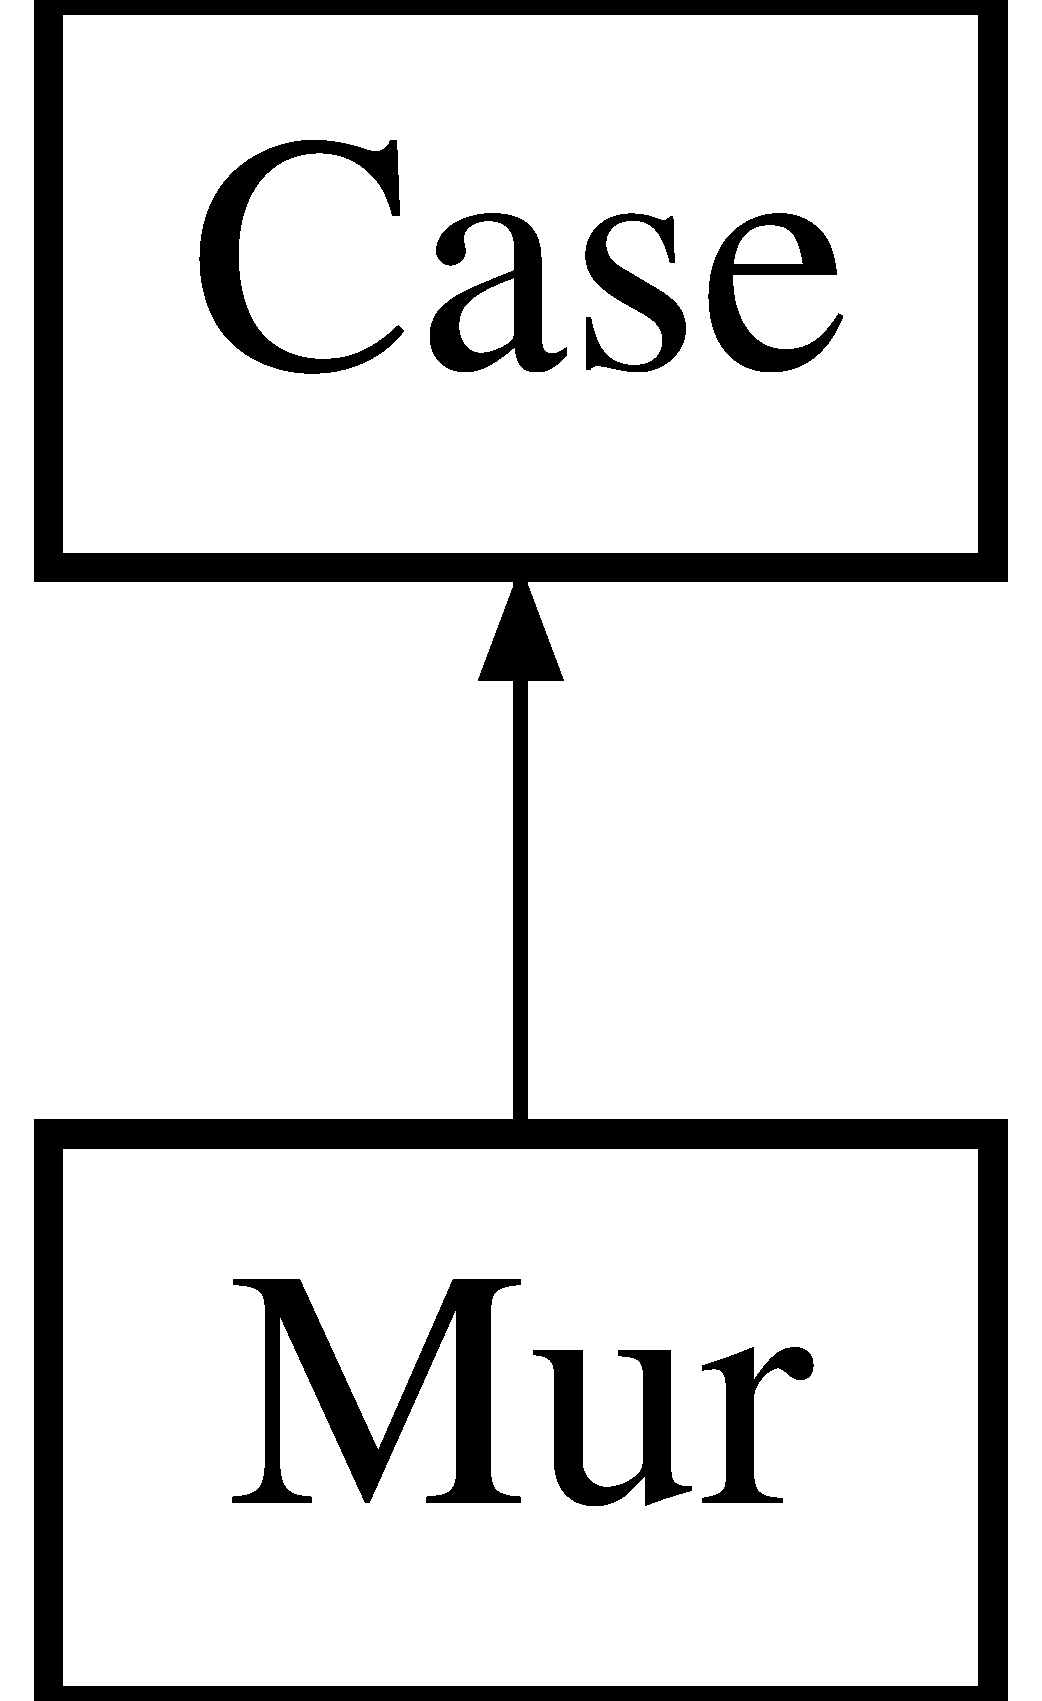
\includegraphics[height=2.000000cm]{classMur}
\end{center}
\end{figure}
\subsection*{\-Fonctions membres publiques}
\begin{DoxyCompactItemize}
\item 
\hypertarget{classMur_a3e7b1afaccb62ba5fa7cc8e1728e7dff}{{\bfseries \-Mur} (int a, int b)}\label{classMur_a3e7b1afaccb62ba5fa7cc8e1728e7dff}

\item 
\hypertarget{classMur_a0fda0e8825c34a5f06d651e263bff058}{virtual std\-::string \hyperlink{classMur_a0fda0e8825c34a5f06d651e263bff058}{action} ()}\label{classMur_a0fda0e8825c34a5f06d651e263bff058}

\begin{DoxyCompactList}\small\item\em \-Methode qui va réaliser l'action selon la case. \end{DoxyCompactList}\item 
virtual std\-::string \hyperlink{classMur_a8d319947a0158801579dc5f1f8568281}{to\-String} ()
\begin{DoxyCompactList}\small\item\em \-Méthode qui retrourne une string repésentant la case du type\-: \mbox{[}x\mbox{]}\mbox{[}y\mbox{]}. \end{DoxyCompactList}\item 
virtual void \hyperlink{classMur_a83a304537e5863c25ce60879196d8e6e}{trouver\-Chemin} (int de, vector$<$ \hyperlink{classCase}{\-Case} $\ast$ $>$ \&res, \hyperlink{classPlateau}{\-Plateau} $\ast$p)
\begin{DoxyCompactList}\small\item\em \-Methode qui trouve tous les chemins possibles. \end{DoxyCompactList}\end{DoxyCompactItemize}


\subsection{\-Description détaillée}
\hyperlink{classMur}{\-Mur} est la classe abstraite représentant les murs les positions ou on ne peut pas deplacer. 

\begin{DoxyAuthor}{\-Auteur}
\-Olivia \-Bruce 

\-Cassandre \-Gloria 
\end{DoxyAuthor}
\begin{DoxyVersion}{\-Version}
1.\-0 
\end{DoxyVersion}


\subsection{\-Documentation des fonctions membres}
\hypertarget{classMur_a8d319947a0158801579dc5f1f8568281}{\index{\-Mur@{\-Mur}!to\-String@{to\-String}}
\index{to\-String@{to\-String}!Mur@{\-Mur}}
\subsubsection[{to\-String}]{\setlength{\rightskip}{0pt plus 5cm}std\-::string {\bf \-Mur\-::to\-String} (
\begin{DoxyParamCaption}
{}
\end{DoxyParamCaption}
)\hspace{0.3cm}{\ttfamily  \mbox{[}virtual\mbox{]}}}}\label{classMur_a8d319947a0158801579dc5f1f8568281}


\-Méthode qui retrourne une string repésentant la case du type\-: \mbox{[}x\mbox{]}\mbox{[}y\mbox{]}. 

\begin{DoxyReturn}{\-Renvoie}
res l'emplacement de la case 
\end{DoxyReturn}


\-Réimplémentée à partir de \hyperlink{classCase_ad09ca1072f39bcacf06459fc03f026ae}{\-Case}.

\hypertarget{classMur_a83a304537e5863c25ce60879196d8e6e}{\index{\-Mur@{\-Mur}!trouver\-Chemin@{trouver\-Chemin}}
\index{trouver\-Chemin@{trouver\-Chemin}!Mur@{\-Mur}}
\subsubsection[{trouver\-Chemin}]{\setlength{\rightskip}{0pt plus 5cm}void {\bf \-Mur\-::trouver\-Chemin} (
\begin{DoxyParamCaption}
\item[{int}]{de, }
\item[{vector$<$ {\bf \-Case} $\ast$ $>$ \&}]{res, }
\item[{{\bf \-Plateau} $\ast$}]{p}
\end{DoxyParamCaption}
)\hspace{0.3cm}{\ttfamily  \mbox{[}virtual\mbox{]}}}}\label{classMur_a83a304537e5863c25ce60879196d8e6e}


\-Methode qui trouve tous les chemins possibles. 


\begin{DoxyParams}{\-Paramètres}
{\em de} & le nombre a parcourir \\
\hline
{\em res} & le vetor des chemins \\
\hline
{\em p} & le plateau \\
\hline
\end{DoxyParams}


\-La documentation de cette classe a été générée à partir des fichiers suivants \-:\begin{DoxyCompactItemize}
\item 
\-Mur.\-h\item 
\-Mur.\-cpp\end{DoxyCompactItemize}

\hypertarget{classObservable}{\section{\-Référence de la classe \-Observable}
\label{classObservable}\index{\-Observable@{\-Observable}}
}


\hyperlink{classObservable}{\-Observable} est la classe abstraite représentant le sujet observer.  




{\ttfamily \#include $<$\-Observable.\-h$>$}

\-Graphe d'héritage de \-Observable\-:\begin{figure}[H]
\begin{center}
\leavevmode
\includegraphics[height=2.000000cm]{classObservable}
\end{center}
\end{figure}
\subsection*{\-Fonctions membres publiques}
\begin{DoxyCompactItemize}
\item 
\hypertarget{classObservable_a02a760ccb777fc6b62b94bb9f6ed75ae}{virtual void {\bfseries ajouter\-Obs} (\hyperlink{classObserver}{\-Observer} $\ast$obs)=0}\label{classObservable_a02a760ccb777fc6b62b94bb9f6ed75ae}

\item 
\hypertarget{classObservable_af60bd92dedfc8befac0cc4fab2845846}{virtual void {\bfseries enlever\-Obs} (\hyperlink{classObserver}{\-Observer} $\ast$obs)=0}\label{classObservable_af60bd92dedfc8befac0cc4fab2845846}

\item 
\hypertarget{classObservable_a0ebba92c40eb637c53346e088cd79880}{virtual void {\bfseries notify\-Obs} ()=0}\label{classObservable_a0ebba92c40eb637c53346e088cd79880}

\end{DoxyCompactItemize}


\subsection{\-Description détaillée}
\hyperlink{classObservable}{\-Observable} est la classe abstraite représentant le sujet observer. 

\-Elle est caractérisé par les informations suivantes \-: une methode ajouter un observateur une methode supprimer un observateur une methode notifier un observateur

\begin{DoxyAuthor}{\-Auteur}
\-Olivia \-Bruce 

\-Cassandre \-Gloria 
\end{DoxyAuthor}
\begin{DoxyVersion}{\-Version}
1.\-0 
\end{DoxyVersion}


\-La documentation de cette classe a été générée à partir du fichier suivant \-:\begin{DoxyCompactItemize}
\item 
\-Observable.\-h\end{DoxyCompactItemize}

\hypertarget{classObserver}{\section{\-Référence de la classe \-Observer}
\label{classObserver}\index{\-Observer@{\-Observer}}
}


\hyperlink{classObserver}{\-Observer} est la classe abstraite représentant l'observer abstrait.  




{\ttfamily \#include $<$\-Observer.\-h$>$}

\-Graphe d'héritage de \-Observer\-:\begin{figure}[H]
\begin{center}
\leavevmode
\includegraphics[height=2.000000cm]{classObserver}
\end{center}
\end{figure}
\subsection*{\-Fonctions membres publiques}
\begin{DoxyCompactItemize}
\item 
\hypertarget{classObserver_ada9b4853829cf3806379037cf4e6fcc6}{virtual void {\bfseries est\-Notifie} (std\-::string choix1, std\-::string choix2, std\-::string act)=0}\label{classObserver_ada9b4853829cf3806379037cf4e6fcc6}

\end{DoxyCompactItemize}


\subsection{\-Description détaillée}
\hyperlink{classObserver}{\-Observer} est la classe abstraite représentant l'observer abstrait. 

\begin{DoxyAuthor}{\-Auteur}
\-Olivia \-Bruce 

\-Cassandre \-Gloria 
\end{DoxyAuthor}
\begin{DoxyVersion}{\-Version}
1.\-0 
\end{DoxyVersion}


\-La documentation de cette classe a été générée à partir du fichier suivant \-:\begin{DoxyCompactItemize}
\item 
\-Observer.\-h\end{DoxyCompactItemize}

\hypertarget{classPartie}{\section{\-Référence de la classe \-Partie}
\label{classPartie}\index{\-Partie@{\-Partie}}
}


\hyperlink{classPartie}{\-Partie} est la classe représentant les cases d'une piece.  




{\ttfamily \#include $<$\-Partie.\-h$>$}

\-Graphe d'héritage de \-Partie\-:\begin{figure}[H]
\begin{center}
\leavevmode
\includegraphics[height=2.000000cm]{classPartie}
\end{center}
\end{figure}
\subsection*{\-Fonctions membres publiques}
\begin{DoxyCompactItemize}
\item 
\hypertarget{classPartie_a1d763e94586edfdaa54cce895287f695}{{\bfseries \-Partie} (\hyperlink{classPlateau}{\-Plateau} $\ast$plat, \hyperlink{classZoneAffichageTexte}{\-Zone\-Affichage\-Texte} $\ast$zone\-T, \hyperlink{classZoneCarte}{\-Zone\-Carte} $\ast$zone\-C, \hyperlink{classZoneChecklist}{\-Zone\-Checklist} $\ast$z, \hyperlink{classDonneesJeu}{\-Donnees\-Jeu} $\ast$d)}\label{classPartie_a1d763e94586edfdaa54cce895287f695}

\item 
\hypertarget{classPartie_ab76c25c57551613a708ab39816d14a9a}{void \hyperlink{classPartie_ab76c25c57551613a708ab39816d14a9a}{preparer} ()}\label{classPartie_ab76c25c57551613a708ab39816d14a9a}

\begin{DoxyCompactList}\small\item\em \-Fonction preparer. \end{DoxyCompactList}\item 
void \hyperlink{classPartie_a2c868f423c455e1aa0aebc9f3482cf8d}{update} (sf\-::\-Event event)
\begin{DoxyCompactList}\small\item\em \-Fonction updatant la partieselon la poistion du clique. \end{DoxyCompactList}\item 
void \hyperlink{classPartie_a2c00254bdd417a300342d1ba1eb5cec3}{afficher} (sf\-::\-Render\-Window \&window)
\begin{DoxyCompactList}\small\item\em \-Fonction d'affichage de la partie selon la poistion du clique. \end{DoxyCompactList}\item 
virtual void \hyperlink{classPartie_a39dcf2ff1dc8f4c7c81edea5e4f2cde8}{est\-Notifie} (std\-::string choix1, std\-::string choix2, std\-::string act)
\begin{DoxyCompactList}\small\item\em \-Fonction notify. \end{DoxyCompactList}\end{DoxyCompactItemize}


\subsection{\-Description détaillée}
\hyperlink{classPartie}{\-Partie} est la classe représentant les cases d'une piece. 

\-Une \hyperlink{classPiece}{\-Piece} est caractérisé par les informations suivantes \-: un accès au données

\begin{DoxyAuthor}{\-Auteur}
\-Olivia \-Bruce 

\-Cassandre \-Gloria 
\end{DoxyAuthor}
\begin{DoxyVersion}{\-Version}
1.\-0 
\end{DoxyVersion}


\subsection{\-Documentation des fonctions membres}
\hypertarget{classPartie_a2c00254bdd417a300342d1ba1eb5cec3}{\index{\-Partie@{\-Partie}!afficher@{afficher}}
\index{afficher@{afficher}!Partie@{\-Partie}}
\subsubsection[{afficher}]{\setlength{\rightskip}{0pt plus 5cm}void {\bf \-Partie\-::afficher} (
\begin{DoxyParamCaption}
\item[{sf\-::\-Render\-Window \&}]{window}
\end{DoxyParamCaption}
)}}\label{classPartie_a2c00254bdd417a300342d1ba1eb5cec3}


\-Fonction d'affichage de la partie selon la poistion du clique. 


\begin{DoxyParams}{\-Paramètres}
{\em une} & xindow \\
\hline
\end{DoxyParams}
\hypertarget{classPartie_a39dcf2ff1dc8f4c7c81edea5e4f2cde8}{\index{\-Partie@{\-Partie}!est\-Notifie@{est\-Notifie}}
\index{est\-Notifie@{est\-Notifie}!Partie@{\-Partie}}
\subsubsection[{est\-Notifie}]{\setlength{\rightskip}{0pt plus 5cm}void {\bf \-Partie\-::est\-Notifie} (
\begin{DoxyParamCaption}
\item[{std\-::string}]{choix1, }
\item[{std\-::string}]{choix2, }
\item[{std\-::string}]{act}
\end{DoxyParamCaption}
)\hspace{0.3cm}{\ttfamily  \mbox{[}virtual\mbox{]}}}}\label{classPartie_a39dcf2ff1dc8f4c7c81edea5e4f2cde8}


\-Fonction notify. 


\begin{DoxyParams}{\-Paramètres}
{\em choix1} & le nom de la carte choisi en premier \\
\hline
{\em choix2} & le nom de la carte choisi en second \\
\hline
{\em act} & a ou s selon si accuse ou soupconne \\
\hline
\end{DoxyParams}


\-Implémente \hyperlink{classObserver}{\-Observer}.

\hypertarget{classPartie_a2c868f423c455e1aa0aebc9f3482cf8d}{\index{\-Partie@{\-Partie}!update@{update}}
\index{update@{update}!Partie@{\-Partie}}
\subsubsection[{update}]{\setlength{\rightskip}{0pt plus 5cm}void {\bf \-Partie\-::update} (
\begin{DoxyParamCaption}
\item[{sf\-::\-Event}]{event}
\end{DoxyParamCaption}
)}}\label{classPartie_a2c868f423c455e1aa0aebc9f3482cf8d}


\-Fonction updatant la partieselon la poistion du clique. 


\begin{DoxyParams}{\-Paramètres}
{\em un} & event \\
\hline
\end{DoxyParams}


\-La documentation de cette classe a été générée à partir des fichiers suivants \-:\begin{DoxyCompactItemize}
\item 
\-Partie.\-h\item 
\-Partie.\-cpp\end{DoxyCompactItemize}

\hypertarget{classPersonnage}{\section{\-Référence de la classe \-Personnage}
\label{classPersonnage}\index{\-Personnage@{\-Personnage}}
}


\hyperlink{classPersonnage}{\-Personnage} est la classe représentant les cases d'une piece.  




{\ttfamily \#include $<$\-Personnage.\-h$>$}

\subsection*{\-Fonctions membres publiques}
\begin{DoxyCompactItemize}
\item 
\hyperlink{classPersonnage_a32ab14d53d8d1c5715af691b494fc9b1}{\-Personnage} (std\-::string nom, std\-::string couleur, std\-::string pion)
\begin{DoxyCompactList}\small\item\em \-Constructeur. \end{DoxyCompactList}\item 
\hypertarget{classPersonnage_a40dce2ec7abb60ec4b069c614e85c813}{bool \hyperlink{classPersonnage_a40dce2ec7abb60ec4b069c614e85c813}{operator==} (\hyperlink{classPersonnage}{\-Personnage} const \&p2)}\label{classPersonnage_a40dce2ec7abb60ec4b069c614e85c813}

\begin{DoxyCompactList}\small\item\em operateur d'egalite \end{DoxyCompactList}\item 
void \hyperlink{classPersonnage_a09a6d250d12b7cde72cef60d6153977d}{set\-Position\-Depart} (\hyperlink{classCase}{\-Case} $\ast$cas)
\begin{DoxyCompactList}\small\item\em \-Rentre la position de dep. \end{DoxyCompactList}\item 
\hyperlink{classCase}{\-Case} $\ast$ \hyperlink{classPersonnage_a94665cc5f3d0e5d3b30e1039d7970f8c}{get\-Position\-Depart} ()
\begin{DoxyCompactList}\small\item\em \-Recupere la position de dep. \end{DoxyCompactList}\item 
std\-::string \hyperlink{classPersonnage_a519301399a9bee1557858aa50a04a85a}{get\-Nom} ()
\begin{DoxyCompactList}\small\item\em \-Recupere le nom du personnage. \end{DoxyCompactList}\item 
std\-::string \hyperlink{classPersonnage_aebbd390a61c946de43685c810d579c42}{get\-Couleur} ()
\begin{DoxyCompactList}\small\item\em \-Recupere la couleur. \end{DoxyCompactList}\item 
std\-::string \hyperlink{classPersonnage_a56fdaf04ef2cebf901c01b284f81f67b}{get\-Pion} ()
\begin{DoxyCompactList}\small\item\em \-Recupere le chemin menant a l'image du pion. \end{DoxyCompactList}\end{DoxyCompactItemize}


\subsection{\-Description détaillée}
\hyperlink{classPersonnage}{\-Personnage} est la classe représentant les cases d'une piece. 

\-Un \hyperlink{classPersonnage}{\-Personnage} est caractérisé par les informations suivantes \-: un nom un chemin vers l'image une position de depart case$\ast$

\begin{DoxyAuthor}{\-Auteur}
\-Olivia \-Bruce 

\-Cassandre \-Gloria 
\end{DoxyAuthor}
\begin{DoxyVersion}{\-Version}
1.\-0 
\end{DoxyVersion}


\subsection{\-Documentation des constructeurs et destructeur}
\hypertarget{classPersonnage_a32ab14d53d8d1c5715af691b494fc9b1}{\index{\-Personnage@{\-Personnage}!\-Personnage@{\-Personnage}}
\index{\-Personnage@{\-Personnage}!Personnage@{\-Personnage}}
\subsubsection[{\-Personnage}]{\setlength{\rightskip}{0pt plus 5cm}{\bf \-Personnage\-::\-Personnage} (
\begin{DoxyParamCaption}
\item[{std\-::string}]{nom, }
\item[{std\-::string}]{couleur, }
\item[{std\-::string}]{pion}
\end{DoxyParamCaption}
)}}\label{classPersonnage_a32ab14d53d8d1c5715af691b494fc9b1}


\-Constructeur. 


\begin{DoxyParams}{\-Paramètres}
{\em n} & un nom \\
\hline
{\em c} & la couleur \\
\hline
{\em pio} & le chemin du pion \\
\hline
\end{DoxyParams}


\subsection{\-Documentation des fonctions membres}
\hypertarget{classPersonnage_aebbd390a61c946de43685c810d579c42}{\index{\-Personnage@{\-Personnage}!get\-Couleur@{get\-Couleur}}
\index{get\-Couleur@{get\-Couleur}!Personnage@{\-Personnage}}
\subsubsection[{get\-Couleur}]{\setlength{\rightskip}{0pt plus 5cm}string {\bf \-Personnage\-::get\-Couleur} (
\begin{DoxyParamCaption}
{}
\end{DoxyParamCaption}
)}}\label{classPersonnage_aebbd390a61c946de43685c810d579c42}


\-Recupere la couleur. 

\begin{DoxyReturn}{\-Renvoie}
couleur 
\end{DoxyReturn}
\hypertarget{classPersonnage_a519301399a9bee1557858aa50a04a85a}{\index{\-Personnage@{\-Personnage}!get\-Nom@{get\-Nom}}
\index{get\-Nom@{get\-Nom}!Personnage@{\-Personnage}}
\subsubsection[{get\-Nom}]{\setlength{\rightskip}{0pt plus 5cm}string {\bf \-Personnage\-::get\-Nom} (
\begin{DoxyParamCaption}
{}
\end{DoxyParamCaption}
)}}\label{classPersonnage_a519301399a9bee1557858aa50a04a85a}


\-Recupere le nom du personnage. 

\begin{DoxyReturn}{\-Renvoie}
nom 
\end{DoxyReturn}
\hypertarget{classPersonnage_a56fdaf04ef2cebf901c01b284f81f67b}{\index{\-Personnage@{\-Personnage}!get\-Pion@{get\-Pion}}
\index{get\-Pion@{get\-Pion}!Personnage@{\-Personnage}}
\subsubsection[{get\-Pion}]{\setlength{\rightskip}{0pt plus 5cm}string {\bf \-Personnage\-::get\-Pion} (
\begin{DoxyParamCaption}
{}
\end{DoxyParamCaption}
)}}\label{classPersonnage_a56fdaf04ef2cebf901c01b284f81f67b}


\-Recupere le chemin menant a l'image du pion. 

\begin{DoxyReturn}{\-Renvoie}
nom 
\end{DoxyReturn}
\hypertarget{classPersonnage_a94665cc5f3d0e5d3b30e1039d7970f8c}{\index{\-Personnage@{\-Personnage}!get\-Position\-Depart@{get\-Position\-Depart}}
\index{get\-Position\-Depart@{get\-Position\-Depart}!Personnage@{\-Personnage}}
\subsubsection[{get\-Position\-Depart}]{\setlength{\rightskip}{0pt plus 5cm}{\bf \-Case} $\ast$ {\bf \-Personnage\-::get\-Position\-Depart} (
\begin{DoxyParamCaption}
{}
\end{DoxyParamCaption}
)}}\label{classPersonnage_a94665cc5f3d0e5d3b30e1039d7970f8c}


\-Recupere la position de dep. 

\begin{DoxyReturn}{\-Renvoie}
cas la case de depart 
\end{DoxyReturn}
\hypertarget{classPersonnage_a09a6d250d12b7cde72cef60d6153977d}{\index{\-Personnage@{\-Personnage}!set\-Position\-Depart@{set\-Position\-Depart}}
\index{set\-Position\-Depart@{set\-Position\-Depart}!Personnage@{\-Personnage}}
\subsubsection[{set\-Position\-Depart}]{\setlength{\rightskip}{0pt plus 5cm}void {\bf \-Personnage\-::set\-Position\-Depart} (
\begin{DoxyParamCaption}
\item[{{\bf \-Case} $\ast$}]{cas}
\end{DoxyParamCaption}
)}}\label{classPersonnage_a09a6d250d12b7cde72cef60d6153977d}


\-Rentre la position de dep. 


\begin{DoxyParams}{\-Paramètres}
{\em cas} & la case de depart \\
\hline
\end{DoxyParams}


\-La documentation de cette classe a été générée à partir des fichiers suivants \-:\begin{DoxyCompactItemize}
\item 
\-Personnage.\-h\item 
\-Personnage.\-cpp\end{DoxyCompactItemize}

\hypertarget{classPiece}{\section{\-Référence de la classe \-Piece}
\label{classPiece}\index{\-Piece@{\-Piece}}
}
\-Graphe d'héritage de \-Piece\-:\begin{figure}[H]
\begin{center}
\leavevmode
\includegraphics[height=3.000000cm]{classPiece}
\end{center}
\end{figure}
\subsection*{\-Fonctions membres publiques}
\begin{DoxyCompactItemize}
\item 
\hypertarget{classPiece_a81b2270c38239330249ed0e3188071ce}{{\bfseries \-Piece} (std\-::string n)}\label{classPiece_a81b2270c38239330249ed0e3188071ce}

\item 
\hypertarget{classPiece_a853e5114a396a009ff046af8e3ba6f5b}{{\bfseries \-Piece} (int a, int b, std\-::string n)}\label{classPiece_a853e5114a396a009ff046af8e3ba6f5b}

\item 
\hypertarget{classPiece_ae2bbb51808f5d87be1761df503571e0d}{virtual std\-::string \hyperlink{classPiece_ae2bbb51808f5d87be1761df503571e0d}{action} ()}\label{classPiece_ae2bbb51808f5d87be1761df503571e0d}

\begin{DoxyCompactList}\small\item\em \-Methode qui va réaliser l'action selon la case. \end{DoxyCompactList}\item 
virtual string \hyperlink{classPiece_ae18523c400cb72a50bb1293d27cd1432}{to\-String} ()
\begin{DoxyCompactList}\small\item\em \-Méthode qui retrourne une string repésentant la case du type\-: \mbox{[}x\mbox{]}\mbox{[}y\mbox{]}. \end{DoxyCompactList}\item 
virtual void \hyperlink{classPiece_ab8f478c95ba4d853c9016d19211e2be1}{trouver\-Chemin} (int de, vector$<$ \hyperlink{classCase}{\-Case} $\ast$ $>$ \&res, \hyperlink{classPlateau}{\-Plateau} $\ast$p)
\begin{DoxyCompactList}\small\item\em \-Methode qui trouve tous les chemins possibles. \end{DoxyCompactList}\item 
\hypertarget{classPiece_afd9fcbb17752f925bd3104acbf271190}{void {\bfseries set\-Porte} (\hyperlink{classPorte}{\-Porte} $\ast$p)}\label{classPiece_afd9fcbb17752f925bd3104acbf271190}

\end{DoxyCompactItemize}
\subsection*{\-Attributs protégés}
\begin{DoxyCompactItemize}
\item 
\hypertarget{classPiece_ad6f31cca0e9343e1ea56cfaf990f3f1e}{string {\bfseries nom\-\_\-}}\label{classPiece_ad6f31cca0e9343e1ea56cfaf990f3f1e}

\item 
\hypertarget{classPiece_ab75a6524350e4e783f7f4980d47e9e02}{\hyperlink{classPorte}{\-Porte} $\ast$ {\bfseries porte}}\label{classPiece_ab75a6524350e4e783f7f4980d47e9e02}

\end{DoxyCompactItemize}


\subsection{\-Documentation des fonctions membres}
\hypertarget{classPiece_ae18523c400cb72a50bb1293d27cd1432}{\index{\-Piece@{\-Piece}!to\-String@{to\-String}}
\index{to\-String@{to\-String}!Piece@{\-Piece}}
\subsubsection[{to\-String}]{\setlength{\rightskip}{0pt plus 5cm}std\-::string {\bf \-Piece\-::to\-String} (
\begin{DoxyParamCaption}
{}
\end{DoxyParamCaption}
)\hspace{0.3cm}{\ttfamily  \mbox{[}virtual\mbox{]}}}}\label{classPiece_ae18523c400cb72a50bb1293d27cd1432}


\-Méthode qui retrourne une string repésentant la case du type\-: \mbox{[}x\mbox{]}\mbox{[}y\mbox{]}. 

\begin{DoxyReturn}{\-Renvoie}
res l'emplacement de la case 
\end{DoxyReturn}


\-Réimplémentée à partir de \hyperlink{classCase_ad09ca1072f39bcacf06459fc03f026ae}{\-Case}.



\-Réimplémentée dans \hyperlink{classPorte_ace3891879a69f2d29ade65d71d869377}{\-Porte}.

\hypertarget{classPiece_ab8f478c95ba4d853c9016d19211e2be1}{\index{\-Piece@{\-Piece}!trouver\-Chemin@{trouver\-Chemin}}
\index{trouver\-Chemin@{trouver\-Chemin}!Piece@{\-Piece}}
\subsubsection[{trouver\-Chemin}]{\setlength{\rightskip}{0pt plus 5cm}void {\bf \-Piece\-::trouver\-Chemin} (
\begin{DoxyParamCaption}
\item[{int}]{de, }
\item[{vector$<$ {\bf \-Case} $\ast$ $>$ \&}]{res, }
\item[{{\bf \-Plateau} $\ast$}]{p}
\end{DoxyParamCaption}
)\hspace{0.3cm}{\ttfamily  \mbox{[}virtual\mbox{]}}}}\label{classPiece_ab8f478c95ba4d853c9016d19211e2be1}


\-Methode qui trouve tous les chemins possibles. 


\begin{DoxyParams}{\-Paramètres}
{\em de} & le nombre a parcourir \\
\hline
{\em res} & le vetor des chemins \\
\hline
{\em p} & le plateau \\
\hline
\end{DoxyParams}


\-Réimplémentée dans \hyperlink{classPorte_a2029ca8cf88e282a6c0a55c49317b738}{\-Porte}.



\-La documentation de cette classe a été générée à partir des fichiers suivants \-:\begin{DoxyCompactItemize}
\item 
\-Piece.\-h\item 
\-Piece.\-cpp\end{DoxyCompactItemize}

\hypertarget{classPlateau}{\section{\-Référence de la classe \-Plateau}
\label{classPlateau}\index{\-Plateau@{\-Plateau}}
}


\hyperlink{classPlateau}{\-Plateau} est la classe représentant le plateau de jeu.  




{\ttfamily \#include $<$\-Plateau.\-h$>$}

\subsection*{\-Fonctions membres publiques}
\begin{DoxyCompactItemize}
\item 
\hypertarget{classPlateau_a0e6ae72e4d7e9923f996c1247e6a6c8b}{virtual \hyperlink{classPlateau_a0e6ae72e4d7e9923f996c1247e6a6c8b}{$\sim$\-Plateau} ()}\label{classPlateau_a0e6ae72e4d7e9923f996c1247e6a6c8b}

\begin{DoxyCompactList}\small\item\em \-Destructeur. \end{DoxyCompactList}\item 
\hypertarget{classPlateau_a122c12319a8843a493fa06fe4f6e55d4}{void \hyperlink{classPlateau_a122c12319a8843a493fa06fe4f6e55d4}{afficher} ()}\label{classPlateau_a122c12319a8843a493fa06fe4f6e55d4}

\begin{DoxyCompactList}\small\item\em \-Methode qui affiche la structure du plateau \-Affichage d'erreur. \end{DoxyCompactList}\item 
void \hyperlink{classPlateau_a583f37e119a4951cb03b9e5f9ed5b253}{afficher} (sf\-::\-Render\-Window \&window)
\begin{DoxyCompactList}\small\item\em \-Methode qui affiche l'image du plateau \-Affichage de l'interface. \end{DoxyCompactList}\item 
bool \hyperlink{classPlateau_a455da594b748a1bbd616537cfb6c5cd5}{position\-Valide} (int x, int y)
\begin{DoxyCompactList}\small\item\em \-Methode qui renvoie si la position de la souris est sur le plateau. \end{DoxyCompactList}\item 
bool \hyperlink{classPlateau_a2feeabd9398101b680bc647fb79b5271}{case\-Valide} (int x, int y)
\begin{DoxyCompactList}\small\item\em \-Pour \hyperlink{classCase_affe73b57a2c81e2f09dc5db45893db3c}{\-Case\-::trouver\-Chemin} verifie si on ne depasse pas les bords du tableau. \end{DoxyCompactList}\item 
\hyperlink{classCase}{\-Case} $\ast$ \hyperlink{classPlateau_ae53f9bb42a1689cb628e7075da5fdb47}{trouver\-Case} (int x, int y)
\begin{DoxyCompactList}\small\item\em \-Renvoi la case du plateau à la position correspondante niveau graphique. \end{DoxyCompactList}\item 
\hyperlink{classCase}{\-Case} $\ast$ \hyperlink{classPlateau_a009b129c0afc68b42ac80a7b0db92d52}{get\-Case} (int x, int y)
\begin{DoxyCompactList}\small\item\em \-Retourne un pointeur vers une case du tableau. \end{DoxyCompactList}\end{DoxyCompactItemize}


\subsection{\-Description détaillée}
\hyperlink{classPlateau}{\-Plateau} est la classe représentant le plateau de jeu. 

\-Un \hyperlink{classPlateau}{\-Plateau} est caractérisé par les informations suivantes \-: un tableau à double dimension de case. une largeur/hauteur

\begin{DoxyAuthor}{\-Auteur}
\-Olivia \-Bruce 

\-Cassandre \-Gloria 
\end{DoxyAuthor}
\begin{DoxyVersion}{\-Version}
1.\-0 
\end{DoxyVersion}


\subsection{\-Documentation des fonctions membres}
\hypertarget{classPlateau_a583f37e119a4951cb03b9e5f9ed5b253}{\index{\-Plateau@{\-Plateau}!afficher@{afficher}}
\index{afficher@{afficher}!Plateau@{\-Plateau}}
\subsubsection[{afficher}]{\setlength{\rightskip}{0pt plus 5cm}void {\bf \-Plateau\-::afficher} (
\begin{DoxyParamCaption}
\item[{sf\-::\-Render\-Window \&}]{window}
\end{DoxyParamCaption}
)}}\label{classPlateau_a583f37e119a4951cb03b9e5f9ed5b253}


\-Methode qui affiche l'image du plateau \-Affichage de l'interface. 


\begin{DoxyParams}{\-Paramètres}
{\em window} & la fenetre de rendu \\
\hline
\end{DoxyParams}
\hypertarget{classPlateau_a2feeabd9398101b680bc647fb79b5271}{\index{\-Plateau@{\-Plateau}!case\-Valide@{case\-Valide}}
\index{case\-Valide@{case\-Valide}!Plateau@{\-Plateau}}
\subsubsection[{case\-Valide}]{\setlength{\rightskip}{0pt plus 5cm}bool {\bf \-Plateau\-::case\-Valide} (
\begin{DoxyParamCaption}
\item[{int}]{x, }
\item[{int}]{y}
\end{DoxyParamCaption}
)}}\label{classPlateau_a2feeabd9398101b680bc647fb79b5271}


\-Pour \hyperlink{classCase_affe73b57a2c81e2f09dc5db45893db3c}{\-Case\-::trouver\-Chemin} verifie si on ne depasse pas les bords du tableau. 


\begin{DoxyParams}{\-Paramètres}
{\em x} & abscisse \\
\hline
{\em y} & ordonnee \\
\hline
\end{DoxyParams}
\begin{DoxyReturn}{\-Renvoie}
si la case est valide 
\end{DoxyReturn}
\hypertarget{classPlateau_a009b129c0afc68b42ac80a7b0db92d52}{\index{\-Plateau@{\-Plateau}!get\-Case@{get\-Case}}
\index{get\-Case@{get\-Case}!Plateau@{\-Plateau}}
\subsubsection[{get\-Case}]{\setlength{\rightskip}{0pt plus 5cm}{\bf \-Case} $\ast$ {\bf \-Plateau\-::get\-Case} (
\begin{DoxyParamCaption}
\item[{int}]{x, }
\item[{int}]{y}
\end{DoxyParamCaption}
)}}\label{classPlateau_a009b129c0afc68b42ac80a7b0db92d52}


\-Retourne un pointeur vers une case du tableau. 


\begin{DoxyParams}{\-Paramètres}
{\em x} & abscisse \\
\hline
{\em y} & ordonnee \\
\hline
\end{DoxyParams}
\begin{DoxyReturn}{\-Renvoie}
une case en x,y 
\end{DoxyReturn}
\hypertarget{classPlateau_a455da594b748a1bbd616537cfb6c5cd5}{\index{\-Plateau@{\-Plateau}!position\-Valide@{position\-Valide}}
\index{position\-Valide@{position\-Valide}!Plateau@{\-Plateau}}
\subsubsection[{position\-Valide}]{\setlength{\rightskip}{0pt plus 5cm}bool {\bf \-Plateau\-::position\-Valide} (
\begin{DoxyParamCaption}
\item[{int}]{x, }
\item[{int}]{y}
\end{DoxyParamCaption}
)}}\label{classPlateau_a455da594b748a1bbd616537cfb6c5cd5}


\-Methode qui renvoie si la position de la souris est sur le plateau. 


\begin{DoxyParams}{\-Paramètres}
{\em x} & abscisse \\
\hline
{\em y} & ordonnee \\
\hline
\end{DoxyParams}
\begin{DoxyReturn}{\-Renvoie}
si la position est valide 
\end{DoxyReturn}
\hypertarget{classPlateau_ae53f9bb42a1689cb628e7075da5fdb47}{\index{\-Plateau@{\-Plateau}!trouver\-Case@{trouver\-Case}}
\index{trouver\-Case@{trouver\-Case}!Plateau@{\-Plateau}}
\subsubsection[{trouver\-Case}]{\setlength{\rightskip}{0pt plus 5cm}{\bf \-Case} $\ast$ {\bf \-Plateau\-::trouver\-Case} (
\begin{DoxyParamCaption}
\item[{int}]{x, }
\item[{int}]{y}
\end{DoxyParamCaption}
)}}\label{classPlateau_ae53f9bb42a1689cb628e7075da5fdb47}


\-Renvoi la case du plateau à la position correspondante niveau graphique. 


\begin{DoxyParams}{\-Paramètres}
{\em x} & abscisse \\
\hline
{\em y} & ordonnee \\
\hline
\end{DoxyParams}


\-La documentation de cette classe a été générée à partir des fichiers suivants \-:\begin{DoxyCompactItemize}
\item 
\-Plateau.\-h\item 
\-Plateau.\-cpp\end{DoxyCompactItemize}

\hypertarget{classPorte}{\section{\-Référence de la classe \-Porte}
\label{classPorte}\index{\-Porte@{\-Porte}}
}


\hyperlink{classPorte}{\-Porte} est la classe représentant l'entree d'une piece et donne accès à toute les cases pièces.  




{\ttfamily \#include $<$\-Porte.\-h$>$}

\-Graphe d'héritage de \-Porte\-:\begin{figure}[H]
\begin{center}
\leavevmode
\includegraphics[height=3.000000cm]{classPorte}
\end{center}
\end{figure}
\subsection*{\-Fonctions membres publiques}
\begin{DoxyCompactItemize}
\item 
\hypertarget{classPorte_a49db32e64af8caf782fe54bffa572d7b}{\hyperlink{classPorte_a49db32e64af8caf782fe54bffa572d7b}{\-Porte} (string nom, \hyperlink{classCase}{\-Case} $\ast$c=\-N\-U\-L\-L)}\label{classPorte_a49db32e64af8caf782fe54bffa572d7b}

\begin{DoxyCompactList}\small\item\em \-Constructeur. \end{DoxyCompactList}\item 
\hypertarget{classPorte_a827b8c0f75a4e19c5763523462c6f224}{\hyperlink{classPorte_a827b8c0f75a4e19c5763523462c6f224}{\-Porte} (string nom, int a, int b, \hyperlink{classCase}{\-Case} $\ast$c=\-N\-U\-L\-L)}\label{classPorte_a827b8c0f75a4e19c5763523462c6f224}

\begin{DoxyCompactList}\small\item\em \-Constructeur. \end{DoxyCompactList}\item 
\hypertarget{classPorte_aa3fdf234c17c43b98bdec5f9d69778a6}{\hyperlink{classPorte_aa3fdf234c17c43b98bdec5f9d69778a6}{\-Porte} (const \hyperlink{classPorte}{\-Porte} \&p, int a, int b)}\label{classPorte_aa3fdf234c17c43b98bdec5f9d69778a6}

\begin{DoxyCompactList}\small\item\em \-Constructeur. \end{DoxyCompactList}\item 
\hypertarget{classPorte_a7b82ccac24bfd8b7fa701f7601328d6c}{virtual \hyperlink{classPorte_a7b82ccac24bfd8b7fa701f7601328d6c}{$\sim$\-Porte} ()}\label{classPorte_a7b82ccac24bfd8b7fa701f7601328d6c}

\begin{DoxyCompactList}\small\item\em \-Destructeur. \end{DoxyCompactList}\item 
void \hyperlink{classPorte_adc13e346f7349fd3dc901ff2197f9106}{ajouter\-Piece} (\hyperlink{classPiece}{\-Piece} $\ast$p)
\begin{DoxyCompactList}\small\item\em \-Methode qui ajoute une piece à la porte. \end{DoxyCompactList}\item 
void \hyperlink{classPorte_ad7f509198fda1bc591bb654b3a3b1fa2}{set\-Chemin\-Secret} (\hyperlink{classCase}{\-Case} $\ast$c)
\begin{DoxyCompactList}\small\item\em \-Modificateur du chemin secret. \end{DoxyCompactList}\item 
\hypertarget{classPorte_ace3891879a69f2d29ade65d71d869377}{virtual string \hyperlink{classPorte_ace3891879a69f2d29ade65d71d869377}{to\-String} ()}\label{classPorte_ace3891879a69f2d29ade65d71d869377}

\begin{DoxyCompactList}\small\item\em \-Affichage d'erreur. \end{DoxyCompactList}\item 
virtual void \hyperlink{classPorte_a2029ca8cf88e282a6c0a55c49317b738}{trouver\-Chemin} (int de, vector$<$ \hyperlink{classCase}{\-Case} $\ast$ $>$ \&res, \hyperlink{classPlateau}{\-Plateau} $\ast$p)
\begin{DoxyCompactList}\small\item\em \-Methode qui trouve tous les chemins possibles. \end{DoxyCompactList}\item 
virtual string \hyperlink{classPorte_a71f6ed526931178c012e8653e609e0e7}{action} ()
\begin{DoxyCompactList}\small\item\em \-Methode qui va réaliser l'action selon la case. \end{DoxyCompactList}\item 
string \hyperlink{classPorte_abeca2ec41fa7476859b90a944736a20a}{get\-Nom} () const 
\begin{DoxyCompactList}\small\item\em \-Retourne le nom de la porte. \end{DoxyCompactList}\end{DoxyCompactItemize}


\subsection{\-Description détaillée}
\hyperlink{classPorte}{\-Porte} est la classe représentant l'entree d'une piece et donne accès à toute les cases pièces. 

\-Une \hyperlink{classPorte}{\-Porte} est caractérisé par les informations suivantes \-: un tableau de piece un pointeur vers case pour un chemin secret

\-Herite de \hyperlink{classPiece}{\-Piece}.

\begin{DoxyAuthor}{\-Auteur}
\-Olivia \-Bruce 

\-Cassandre \-Gloria 
\end{DoxyAuthor}
\begin{DoxyVersion}{\-Version}
1.\-0 
\end{DoxyVersion}


\subsection{\-Documentation des fonctions membres}
\hypertarget{classPorte_a71f6ed526931178c012e8653e609e0e7}{\index{\-Porte@{\-Porte}!action@{action}}
\index{action@{action}!Porte@{\-Porte}}
\subsubsection[{action}]{\setlength{\rightskip}{0pt plus 5cm}std\-::string {\bf \-Porte\-::action} (
\begin{DoxyParamCaption}
{}
\end{DoxyParamCaption}
)\hspace{0.3cm}{\ttfamily  \mbox{[}virtual\mbox{]}}}}\label{classPorte_a71f6ed526931178c012e8653e609e0e7}


\-Methode qui va réaliser l'action selon la case. 

\begin{DoxyReturn}{\-Renvoie}
le nom 
\end{DoxyReturn}


\-Réimplémentée à partir de \hyperlink{classPiece_ae2bbb51808f5d87be1761df503571e0d}{\-Piece}.

\hypertarget{classPorte_adc13e346f7349fd3dc901ff2197f9106}{\index{\-Porte@{\-Porte}!ajouter\-Piece@{ajouter\-Piece}}
\index{ajouter\-Piece@{ajouter\-Piece}!Porte@{\-Porte}}
\subsubsection[{ajouter\-Piece}]{\setlength{\rightskip}{0pt plus 5cm}void {\bf \-Porte\-::ajouter\-Piece} (
\begin{DoxyParamCaption}
\item[{{\bf \-Piece} $\ast$}]{p}
\end{DoxyParamCaption}
)}}\label{classPorte_adc13e346f7349fd3dc901ff2197f9106}


\-Methode qui ajoute une piece à la porte. 


\begin{DoxyParams}{\-Paramètres}
{\em une} & piece a ajouter \\
\hline
\end{DoxyParams}
\hypertarget{classPorte_abeca2ec41fa7476859b90a944736a20a}{\index{\-Porte@{\-Porte}!get\-Nom@{get\-Nom}}
\index{get\-Nom@{get\-Nom}!Porte@{\-Porte}}
\subsubsection[{get\-Nom}]{\setlength{\rightskip}{0pt plus 5cm}string {\bf \-Porte\-::get\-Nom} (
\begin{DoxyParamCaption}
{}
\end{DoxyParamCaption}
) const}}\label{classPorte_abeca2ec41fa7476859b90a944736a20a}


\-Retourne le nom de la porte. 


\begin{DoxyParams}{\-Paramètres}
{\em une} & case pointant vers la porte de l'autre piece \\
\hline
\end{DoxyParams}
\hypertarget{classPorte_ad7f509198fda1bc591bb654b3a3b1fa2}{\index{\-Porte@{\-Porte}!set\-Chemin\-Secret@{set\-Chemin\-Secret}}
\index{set\-Chemin\-Secret@{set\-Chemin\-Secret}!Porte@{\-Porte}}
\subsubsection[{set\-Chemin\-Secret}]{\setlength{\rightskip}{0pt plus 5cm}void {\bf \-Porte\-::set\-Chemin\-Secret} (
\begin{DoxyParamCaption}
\item[{{\bf \-Case} $\ast$}]{c}
\end{DoxyParamCaption}
)}}\label{classPorte_ad7f509198fda1bc591bb654b3a3b1fa2}


\-Modificateur du chemin secret. 

\begin{DoxyReturn}{\-Renvoie}
nom le nom de la porte 
\end{DoxyReturn}
\hypertarget{classPorte_a2029ca8cf88e282a6c0a55c49317b738}{\index{\-Porte@{\-Porte}!trouver\-Chemin@{trouver\-Chemin}}
\index{trouver\-Chemin@{trouver\-Chemin}!Porte@{\-Porte}}
\subsubsection[{trouver\-Chemin}]{\setlength{\rightskip}{0pt plus 5cm}void {\bf \-Porte\-::trouver\-Chemin} (
\begin{DoxyParamCaption}
\item[{int}]{de, }
\item[{vector$<$ {\bf \-Case} $\ast$ $>$ \&}]{res, }
\item[{{\bf \-Plateau} $\ast$}]{p}
\end{DoxyParamCaption}
)\hspace{0.3cm}{\ttfamily  \mbox{[}virtual\mbox{]}}}}\label{classPorte_a2029ca8cf88e282a6c0a55c49317b738}


\-Methode qui trouve tous les chemins possibles. 


\begin{DoxyParams}{\-Paramètres}
{\em de} & le nombre a parcourir \\
\hline
{\em res} & le vetor des chemins \\
\hline
{\em p} & le plateau \\
\hline
\end{DoxyParams}


\-Réimplémentée à partir de \hyperlink{classPiece_ab8f478c95ba4d853c9016d19211e2be1}{\-Piece}.



\-La documentation de cette classe a été générée à partir des fichiers suivants \-:\begin{DoxyCompactItemize}
\item 
\-Porte.\-h\item 
\-Porte.\-cpp\end{DoxyCompactItemize}

\hypertarget{classZoneAffichageTexte}{\section{\-Référence de la classe \-Zone\-Affichage\-Texte}
\label{classZoneAffichageTexte}\index{\-Zone\-Affichage\-Texte@{\-Zone\-Affichage\-Texte}}
}


\hyperlink{classZoneAffichageTexte}{\-Zone\-Affichage\-Texte} est la classe représentant la partie affichant le deroulement du jeu.  




{\ttfamily \#include $<$\-Zone\-Affichage\-Texte.\-h$>$}

\subsection*{\-Fonctions membres publiques}
\begin{DoxyCompactItemize}
\item 
void \hyperlink{classZoneAffichageTexte_a209bb3c8fe4790b63326aee7066aca28}{afficher} (sf\-::\-Render\-Window \&window)
\begin{DoxyCompactList}\small\item\em \-Methode qui affiche le texte. \end{DoxyCompactList}\end{DoxyCompactItemize}


\subsection{\-Description détaillée}
\hyperlink{classZoneAffichageTexte}{\-Zone\-Affichage\-Texte} est la classe représentant la partie affichant le deroulement du jeu. 

\-Classe non fonctionnel \-: probleme sfml sf\-::text

\begin{DoxyAuthor}{\-Auteur}
\-Olivia \-Bruce 

\-Cassandre \-Gloria 
\end{DoxyAuthor}
\begin{DoxyVersion}{\-Version}
1.\-0 
\end{DoxyVersion}


\subsection{\-Documentation des fonctions membres}
\hypertarget{classZoneAffichageTexte_a209bb3c8fe4790b63326aee7066aca28}{\index{\-Zone\-Affichage\-Texte@{\-Zone\-Affichage\-Texte}!afficher@{afficher}}
\index{afficher@{afficher}!ZoneAffichageTexte@{\-Zone\-Affichage\-Texte}}
\subsubsection[{afficher}]{\setlength{\rightskip}{0pt plus 5cm}void {\bf \-Zone\-Affichage\-Texte\-::afficher} (
\begin{DoxyParamCaption}
\item[{sf\-::\-Render\-Window \&}]{window}
\end{DoxyParamCaption}
)}}\label{classZoneAffichageTexte_a209bb3c8fe4790b63326aee7066aca28}


\-Methode qui affiche le texte. 


\begin{DoxyParams}{\-Paramètres}
{\em fenetre} & la fenetre de rendu \\
\hline
\end{DoxyParams}


\-La documentation de cette classe a été générée à partir des fichiers suivants \-:\begin{DoxyCompactItemize}
\item 
\-Zone\-Affichage\-Texte.\-h\item 
\-Zone\-Affichage\-Texte.\-cpp\end{DoxyCompactItemize}

\hypertarget{classZoneCarte}{\section{\-Référence de la classe \-Zone\-Carte}
\label{classZoneCarte}\index{\-Zone\-Carte@{\-Zone\-Carte}}
}
\subsection*{\-Fonctions membres publiques}
\begin{DoxyCompactItemize}
\item 
\hypertarget{classZoneCarte_ae60d85f22bb2dea8e632e947e22c1f79}{void {\bfseries afficher\-Carte} (\hyperlink{classJoueur}{\-Joueur} j, sf\-::\-Render\-Window \&window)}\label{classZoneCarte_ae60d85f22bb2dea8e632e947e22c1f79}

\end{DoxyCompactItemize}


\-La documentation de cette classe a été générée à partir des fichiers suivants \-:\begin{DoxyCompactItemize}
\item 
\-Zone\-Carte.\-h\item 
\-Zone\-Carte.\-cpp\end{DoxyCompactItemize}

\hypertarget{classZoneChecklist}{\section{\-Référence de la classe \-Zone\-Checklist}
\label{classZoneChecklist}\index{\-Zone\-Checklist@{\-Zone\-Checklist}}
}
\subsection*{\-Fonctions membres publiques}
\begin{DoxyCompactItemize}
\item 
\hypertarget{classZoneChecklist_aee5e8750e39ef396f708fdfec48eca8c}{\hyperlink{classZoneChecklist_aee5e8750e39ef396f708fdfec48eca8c}{\-Zone\-Checklist} ()}\label{classZoneChecklist_aee5e8750e39ef396f708fdfec48eca8c}

\begin{DoxyCompactList}\small\item\em \-Constructeur. \end{DoxyCompactList}\item 
\hypertarget{classZoneChecklist_a1ffde7f6689c34844d38c527a87a7740}{virtual \hyperlink{classZoneChecklist_a1ffde7f6689c34844d38c527a87a7740}{$\sim$\-Zone\-Checklist} ()}\label{classZoneChecklist_a1ffde7f6689c34844d38c527a87a7740}

\begin{DoxyCompactList}\small\item\em \-Destructeur. \end{DoxyCompactList}\item 
\hypertarget{classZoneChecklist_a08e07cd3db2e76f1d33a0e3b26ec32eb}{void \hyperlink{classZoneChecklist_a08e07cd3db2e76f1d33a0e3b26ec32eb}{afficher\-Checklist} (\hyperlink{classJoueur}{\-Joueur} $\ast$j, sf\-::\-Render\-Window \&window)}\label{classZoneChecklist_a08e07cd3db2e76f1d33a0e3b26ec32eb}

\begin{DoxyCompactList}\small\item\em afficher\-Checklist \end{DoxyCompactList}\item 
\hypertarget{classZoneChecklist_a5cb52a1aff880ce982ab002cafecce97}{void {\bfseries update} (\hyperlink{classJoueur}{\-Joueur} $\ast$j, sf\-::\-Event event)}\label{classZoneChecklist_a5cb52a1aff880ce982ab002cafecce97}

\item 
\hypertarget{classZoneChecklist_a31c52e893fe409f1dd2860eb9f28ce81}{void \hyperlink{classZoneChecklist_a31c52e893fe409f1dd2860eb9f28ce81}{placer\-Case\-Cocher} (\hyperlink{classBouton}{\-Bouton} b, int y, sf\-::\-Render\-Window \&fenetre)}\label{classZoneChecklist_a31c52e893fe409f1dd2860eb9f28ce81}

\begin{DoxyCompactList}\small\item\em \-Fonction placer\-Case\-Cocher. \end{DoxyCompactList}\item 
\hypertarget{classZoneChecklist_a2d22b4546f136a703da6fb0c6b8c0dcb}{void \hyperlink{classZoneChecklist_a2d22b4546f136a703da6fb0c6b8c0dcb}{actualiser\-Checklist} (\hyperlink{classJoueur}{\-Joueur} $\ast$j)}\label{classZoneChecklist_a2d22b4546f136a703da6fb0c6b8c0dcb}

\begin{DoxyCompactList}\small\item\em \-Fonction placer\-Case\-Cocher. \end{DoxyCompactList}\item 
\hypertarget{classZoneChecklist_a131c733dca0597e4b8a4e24303dc0f25}{void {\bfseries clique\-Conditionnel} (int x, int y, int xmin, int xmax, int ymin, int ymax, \hyperlink{classBouton}{\-Bouton} \&b)}\label{classZoneChecklist_a131c733dca0597e4b8a4e24303dc0f25}

\item 
\hypertarget{classZoneChecklist_ab6600a57c75090d99f2efad6b66a5a93}{void \hyperlink{classZoneChecklist_ab6600a57c75090d99f2efad6b66a5a93}{importation} (\hyperlink{classBouton}{\-Bouton} \&b, int i, vector$<$ bool $>$ vec)}\label{classZoneChecklist_ab6600a57c75090d99f2efad6b66a5a93}

\begin{DoxyCompactList}\small\item\em \-Fonction importation. \end{DoxyCompactList}\end{DoxyCompactItemize}


\-La documentation de cette classe a été générée à partir des fichiers suivants \-:\begin{DoxyCompactItemize}
\item 
\-Zone\-Checklist.\-h\item 
\-Zone\-Checklist.\-cpp\end{DoxyCompactItemize}

\printindex
\end{document}
